% KAIROS conference-paper reconstruction source (~8,000 words)
% Build on Overleaf with pdfLaTeX, or locally with: latexmk -pdf main.tex
% EVIDENCE BOUNDARY: this reconstructs historical manuscript content using a
% generic article layout. It is not the exact source closure of KAIROS_FINAL.pdf,
% and its historical claims remain quarantined by the repository evidence ledger.
\documentclass[11pt]{article}
\usepackage[margin=1in]{geometry}
\usepackage[numbers]{natbib}

% ── Packages ────────────────────────────────────────────────────────────────
\usepackage{amsmath,amssymb,amsfonts,amsthm}
\newtheorem{theorem}{Theorem}
\newtheorem{proposition}[theorem]{Proposition}
\newtheorem{corollary}[theorem]{Corollary}
\newtheorem{lemma}[theorem]{Lemma}
\newtheorem{definition}{Definition}
\newtheorem{remark}{Remark}
\newtheorem{assumption}{Assumption}
\usepackage{graphicx}
\usepackage{booktabs}
\usepackage{multirow}
\usepackage{algorithm}
\usepackage{algorithmic}
\usepackage{microtype}
\usepackage{subcaption}
\usepackage{bm}
\usepackage[hidelinks]{hyperref}

% ── Math commands ───────────────────────────────────────────────────────────
\newcommand{\R}{\mathbb{R}}
\newcommand{\E}{\mathbb{E}}
\newcommand{\KL}{\mathrm{KL}}
\newcommand{\Softmax}{\mathrm{Softmax}}
\newcommand{\GRU}{\mathrm{GRU}}
\newcommand{\CSM}{\mathrm{CSM}}
\newcommand{\RSE}{\mathrm{RSE}}
\newcommand{\RMP}{\mathrm{RMP}}
\newcommand{\SCP}{\mathrm{SCP}}
\newcommand{\TIP}{\mathrm{TIP}}
\newcommand{\CFI}{\mathrm{CFI}}
\newcommand{\SR}{\mathrm{SR}}
\newcommand{\EWS}{\mathrm{EWS}}

% ── Title ───────────────────────────────────────────────────────────────────
\title{KAIROS: Causal Market Intelligence via Resonance Symbolic Graph Neural Networks for Early Detection of Regime Transitions}

\author{
  Duong Viet Hoang\textsuperscript{1} \quad Lun-Min Shih\textsuperscript{1} \quad Yi-Hao Lai\textsuperscript{2} \\[0.3em]
  \textsuperscript{1}Department of Computer Science, Da-Yeh University, Taiwan \\
  \textsuperscript{2}Department of Finance, Da-Yeh University, Taiwan \\[0.2em]
  \texttt{Hoangduong4316@icloud.com} \quad \texttt{Lmshih@mail.dyu.edu.tw} \quad \texttt{yhlai@mail.dyu.edu.tw}
}
\date{}

\begin{document}
\maketitle

% ============================================================================
% ABSTRACT
% ============================================================================
\begin{abstract}
Timely detection of financial regime transitions---such as market crashes or sentiment-driven selloffs---remains a critical challenge, as most existing indicators are inherently lagging and only confirm crises after they have begun. We present \textbf{KAIROS} (\textbf{K}ausal \textbf{AI} for \textbf{R}egime \textbf{O}nset \textbf{S}ensing), an AI-powered causal market intelligence system that leverages \textbf{RS-GNN} (Resonance Symbolic Graph Neural Network) to detect early structural signals of regime transitions before they become observable in price or sentiment data.

KAIROS models financial markets as dynamic causal graphs, where asset clusters are nodes and their evolving dependencies are edges governed by a \emph{Causal State Machine} (CSM) with five symbolic lifecycle states (IDLE$\to$BIRTH$\to$REINFORCE$\to$DECAY$\to$DEATH). The system continuously monitors how these causal relationships form, strengthen, and dissolve over time, using learned neuro-symbolic constraints that encode market physics---ensuring that causal links cannot materialize without first being born. An emergent \emph{Causal Fear Index} (CFI) is automatically derived from the structural resonance of these edge states, requiring zero hand-crafted sentiment rules. Every prediction admits a unique causal trace decomposition (Theorem~3), enabling native counterfactual reasoning: ``Which specific inter-asset relationships are driving the current fear signal?''

Applied to 28~assets and 35~macro causal edges over 11~years, KAIROS achieves 72.3\% balanced accuracy on the blind test set while uniquely providing causal traceability, compliance, auditability, and per-edge risk attribution---capabilities that no existing temporal graph method offers. KAIROS detected the onset of COVID-19 market fear \textbf{25~days} before the CNN Fear~\&~Greed Index. Cross-domain transfer to real COVID-19 epidemiology (15~countries) yields a +21~point improvement over GRU baselines with zero architectural changes---a reversal that validates KAIROS's causal foundations. We propose a \emph{Causal Intelligence} evaluation framework arguing that in domains with external interventions (monetary policy, regulation), classification accuracy alone is confounded and insufficient as a sole evaluation metric.

KAIROS offers a practical, data-driven framework for early financial risk detection, with potential applications in portfolio risk management, systemic risk monitoring, and regulatory compliance.
\end{abstract}

\textbf{Keywords:} Graph Neural Networks $\cdot$ Causal Inference $\cdot$ Regime Detection $\cdot$ Neuro-Symbolic AI $\cdot$ Financial Machine Learning $\cdot$ Early Warning Systems $\cdot$ Counterfactual Reasoning

% ============================================================================
% 1. INTRODUCTION
% ============================================================================
\section{Introduction}

In late January 2020, capital began flowing from cryptocurrency markets into U.S.\ treasuries---Bitcoin dropped 6\% over two weeks while TLT (20-year Treasury ETF) rose 3\%. This structural shift in inter-asset causal flow preceded the S\&P 500 crash by 25 days, yet no existing model detected it: the VIX remained below 15, the CNN Fear \& Greed Index~\citep{cnn_fg} read ``Greed,'' and standard temporal graph networks continued to predict bullish conditions. The causal mechanism---risk capital rotating into safe havens---was already active, but every observable macroscopic indicator remained calm.

These examples illustrate a fundamental limitation of current approaches to regime detection in complex systems. The causal structure of a system changes \emph{before} the macroscopic observables reflect that change, creating a detection gap that purely correlational methods cannot bridge. Complex systems---financial markets, epidemics, climate networks---exhibit \emph{regime transitions}: abrupt shifts in the latent causal structure governing observed dynamics~\citep{scheffer2009early}. Statistical methods for detecting early-warning signals of such critical transitions~\citep{dakos2012methods} have been developed primarily for ecological and climate systems, but they operate on univariate time series and do not model the causal graph structure that drives the transition. Traditional approaches model these systems with two fundamentally limited paradigms.

\paragraph{Paradigm 1: Snapshot-based temporal models.} Existing temporal graph networks~\citep{rossi2020tgn,xu2020tgat,trivedi2019dyrep,cong2023graphmixer} process discrete snapshots of the interaction graph, losing the continuous causal evolution between snapshots. They treat edges as instantaneous observations rather than evolving causal relationships with lifecycles. TGN~\citep{rossi2020tgn} maintains temporal node memory but does not model edge states; TGAT~\citep{xu2020tgat} applies attention over temporal neighborhoods but lacks any notion of edge formation or dissolution; DyRep~\citep{trivedi2019dyrep} models event dynamics but without symbolic constraints on edge evolution. Critically, none of these architectures can distinguish between a newly forming causal link (which carries early-warning information) and an established one (which merely confirms what is already observable). This distinction---between the \emph{birth} and \emph{reinforcement} of a causal dependency---is precisely where early detection resides.

\paragraph{Paradigm 2: Correlational evaluation metrics.} Standard evaluation relies on classification accuracy, which conflates \emph{causal correctness} with \emph{outcome observation}. When external interventions (e.g., central bank quantitative easing, public health lockdowns, circuit breakers) alter outcomes without changing the underlying causal structure, high accuracy can mask causal ignorance, while ``errors'' can reflect genuine causal intelligence. A model that correctly identifies a forming crisis but is scored as ``wrong'' because a central bank intervened to prevent the crash is being penalized for understanding the system better than its evaluation metric can measure. This problem is not merely academic: in March 2020, the Federal Reserve's unlimited QE announcement on March 23 reversed market trajectory within days, meaning any model evaluated purely on next-day returns would be penalized for detecting the genuine structural crisis that precipitated the intervention.

\paragraph{The neuro-symbolic imperative.} Natural complex systems are simultaneously \emph{complex} (requiring neural flexibility to capture nonlinear, high-dimensional dynamics) and \emph{law-governed} (requiring symbolic compliance with structural constraints that reflect domain physics). Financial markets cannot have full contagion without first observing capital flow beginning; epidemics cannot have sustained community spread without initial transmission events; climate systems cannot have regime shifts without preceding changes in energy balance. These are not soft statistical regularities---they are structural laws that constrain the space of possible causal evolutions. A purely neural approach discards this knowledge; a purely symbolic approach cannot handle the complexity. The neuro-symbolic synthesis---neural networks operating within symbolically enforced causal constraints---is not a compromise but a \emph{necessity} for modeling systems where both complexity and law-governance coexist.

\paragraph{Key insight.} Regime transitions manifest first as structural changes in the causal graph---new edges forming (BIRTH), strengthening (REINFORCE), weakening (DECAY), and dissolving (DEATH)---before any macroscopic signal becomes observable. A model that tracks these edge lifecycles can detect regime onset \emph{before} traditional indices react. The temporal gap between BIRTH (when causal flow begins) and macroscopic observation (when aggregate indicators cross thresholds) is the \emph{early detection window} that KAIROS exploits.

\paragraph{Contributions.} We make four contributions:
\begin{enumerate}
    \item \textbf{Theory:} We formulate regime detection as a Temporal Information Parsimony (TIP) problem, proving the optimal compiled graph is the minimal sufficient statistic (Theorem~\ref{thm:optimal}). We establish an early detection bound showing that BIRTH-state counting detects regime onset $\Omega(\log(1/\delta))$ time steps before macroscopic indicators cross threshold $\delta$ (Theorem~\ref{thm:early}). We derive a unique causal trace decomposition enabling edge-level attribution of regime signals (Theorem~\ref{thm:trace}). Together, these results provide, to our knowledge, the first theoretical foundation for early regime detection via causal graph compilation.
    \item \textbf{Architecture:} RS-GNN integrates four differentiable layers---the Resonance Signal Encoder (RSE) with physics-inspired acceleration gating, the Causal State Machine (CSM) with symbolically constrained 5-state lifecycle, Resonance Message Passing (RMP) with Temporal Information Parsimony (TIP) for momentum-conditioned message passing and variational compression, and the Symbolic Causal Policy (SCP) with causally masked regime prediction---in a single end-to-end framework of only 92,388 parameters. The architecture is domain-agnostic: the same model handles financial markets and epidemiology with zero structural changes.
    \item \textbf{Evaluation:} We propose Causal Intelligence (CI), a six-dimensional evaluation framework encompassing classification accuracy, Granger predictive coupling, early detection capability, causal traceability, causal compliance, and anomaly auditability. We prove (Proposition~\ref{prop:confound}) that in domains with non-zero intervention rates, outcome accuracy systematically underestimates the quality of causally correct models, making CI evaluation essential rather than optional.
    \item \textbf{Empirical:} On 28 financial assets over 11 years, KAIROS detects COVID-19 fear \textbf{25 days} before CNN Fear \& Greed Index, with CSM states exhibiting clear lifecycle dynamics: BIRTH edges spike from 0 to 24/35 as capital flight begins, then transition to REINFORCE as fear is confirmed. Cross-domain transfer to COVID-19 epidemiology (15 countries) yields a +21 point balanced accuracy improvement over GRU baseline---a \emph{reversal} from the financial domain that validates the intervention confounding theory.
\end{enumerate}

% ============================================================================
% 2. RELATED WORK
% ============================================================================
\section{Related Work}

\paragraph{Temporal Graph Networks.}
Temporal graph learning has evolved from foundational architectures---GCN~\citep{kipf2017gcn}, GAT~\citep{velickovic2018gat}, and the expressiveness analysis of GIN~\citep{xu2019powerful}---through static GNNs~\citep{he2020lightgcn} and attention-based approaches~\citep{xu2020tgat} to continuous-time models~\citep{rossi2020tgn,trivedi2019dyrep}. Kazemi et al.~\citep{kazemi2020dynamic} provide a comprehensive survey of representation learning for dynamic graphs. TGN~\citep{rossi2020tgn} introduced temporal memory modules that maintain per-node state across interactions, while DyRep~\citep{trivedi2019dyrep} models the temporal point process of edge events. GraphMixer~\citep{cong2023graphmixer} demonstrated that simple MLP-Mixer architectures can match attention-based temporal models, questioning the necessity of complex temporal attention. Recent work has advanced both the theoretical expressiveness~\citep{souza2022provably,yu2023towards} and evaluation methodology~\citep{poursafaei2022towards} of temporal graph networks. However, all these methods treat edges as instantaneous observations---they lack any model of edge \emph{lifecycle} (formation, strengthening, weakening, dissolution). KAIROS's CSM explicitly tracks these phases, enabling detection of regime onset at the BIRTH stage rather than after macroscopic effects become apparent.

\paragraph{Graph Information Bottleneck.}
Information bottleneck methods~\citep{tishby2000ib} compress representations while preserving task-relevant information. GIB~\citep{wu2020gib} applies this principle to graph-structured data, learning compressed subgraphs that retain predictive power. VIB~\citep{alemi2017vib} provides a variational approximation enabling end-to-end training. Multi-view information bottleneck~\citep{federici2020multiview} extends these ideas to learning robust representations across multiple views. KAIROS extends this line of work with \emph{Temporal} Information Parsimony (TIP), which operates on evolving event streams rather than static graphs. The key difference is that TIP must balance compression across time---retaining sufficient causal history to predict future events while discarding temporally redundant information. The variational bottleneck dimension ($d_z = 24$) in KAIROS was selected via grid search over $\{8, 16, 24, 32, 48\}$ on the validation set to match the intrinsic dimensionality of the 35-edge causal graph (Appendix~D).

\paragraph{Neuro-Symbolic AI.}
Neural-symbolic integration~\citep{garcez2019neural_symbolic,lamb2020gnn_neurosymbolic} seeks to combine the learning capacity of neural networks with the reasoning guarantees of symbolic systems. Neural Logic Machines~\citep{dong2019nlm} learn first-order logic rules via differentiable operations, and NeuralLP~\citep{yang2017neurallp} performs differentiable rule learning for knowledge base reasoning. These approaches typically apply symbolic constraints to static knowledge structures. KAIROS brings neuro-symbolic methods to \emph{temporal} causal graphs: the CSM's transition mask $M$ encodes domain-invariant causal laws (e.g., a dependency must form before it can strengthen) as hard constraints within a differentiable architecture. Unlike post-hoc symbolic verification, KAIROS's constraints are embedded in the forward pass, ensuring every prediction is causally compliant by construction.

\paragraph{Financial Regime Detection.}
Hamilton's regime-switching model~\citep{hamilton1989hmm} introduced Hidden Markov Models for economic regime identification, modeling transitions between expansion and contraction states. Subsequent work extended regime-switching to interest rates~\citep{ang2002regime} and asset pricing anomalies~\citep{guidolin2008size}. Cont~\citep{cont2001stylized} established the stylized facts of asset returns---heavy tails, volatility clustering, and leverage effects---that any financial model must accommodate. Machine learning approaches to asset pricing~\citep{gu2020empirical} and financial time series~\citep{bao2017deep,lopezdeprado2018advances} have demonstrated the power of deep learning in capturing nonlinear financial dynamics, but typically operate on individual assets or portfolios without explicit causal structure. Network-based approaches to systemic risk~\citep{diebold2014connectedness,billio2012systemic,acemoglu2015systemic} measure financial connectedness through variance decompositions and Granger-causal linkages, but operate on static or slowly-evolving network snapshots without modeling edge lifecycle dynamics. Financial GNNs~\citep{chen2022financial_gnn,feng2019temporal,sawhney2021stock,cheng2021financial} model risk propagation and stock prediction on asset graphs but operate on fixed topologies without modeling edge dynamics. Spatiotemporal forecasting methods~\citep{li2018dcrnn,yu2018stgcn} capture spatial and temporal dependencies but are designed for stationary processes (traffic flow, weather) rather than regime transitions. KAIROS differs fundamentally by modeling the \emph{lifecycle of inter-asset causal edges} rather than node-level features or static graph properties: the regime is not a hidden state of a single time series but an emergent property of the evolving causal graph structure.

\paragraph{Causal Discovery in Time Series.}
Causal inference has deep roots in structural equation models~\citep{pearl2009causality}, the potential outcomes framework~\citep{imbens2015causal}, marginal structural models for longitudinal data~\citep{robins2000marginal}, and constraint-based discovery algorithms~\citep{spirtes2000causation}. Peters et al.~\citep{peters2017elements} provide a modern treatment of causal learning from observational data, while VanderWeele~\citep{vanderweele2015explanation} develops methods for mediation analysis and causal explanation. Recent surveys~\citep{glymour2019review,assaad2022survey} catalogue the rapidly growing landscape of causal discovery methods, including those designed specifically for time series. Eichler~\citep{eichler2012causal} provides a systematic treatment of causal inference in time series analysis. Sch{\"o}lkopf et al.~\citep{scholkopf2021toward} articulate the vision of causal representation learning---learning representations that respect underlying causal structure rather than mere statistical associations. Granger causality~\citep{granger1969} remains the most widely used test for directional predictability in time series, though it captures linear, pairwise relationships. Neural Granger causality~\citep{tank2022neural_granger} extends this to nonlinear settings. Runge~\citep{runge2018causal} addresses the practical estimation of causal networks from time series under realistic assumptions. PCMCI~\citep{runge2019pcmci} combines the Peter-Clark algorithm with momentary conditional independence tests for high-dimensional causal discovery. Differentiable structure learning methods such as NOTEARS~\citep{zheng2018dags} and DCDI~\citep{brouillard2020differentiable} learn causal DAGs via continuous optimization, while amortized approaches~\citep{lowe2022amortized} learn to infer causal graphs from time-series data in a single forward pass. Deep end-to-end causal inference~\citep{geffner2022deep} and meta-transfer objectives~\citep{bengio2020metatransfer} further bridge causal reasoning with deep learning. Causal interpretability~\citep{moraffah2021causal} addresses the need for models whose predictions can be explained through causal mechanisms. Change point detection methods~\citep{aminikhanghahi2017changepoint,adams2007bocpd} identify regime boundaries but treat each time series independently, without modeling the causal interactions that \emph{produce} the regime change. To our knowledge, KAIROS is the first framework to combine causal discovery (which edges exist), causal state tracking (what lifecycle stage each edge occupies), and causal compilation (compressing the event stream into a minimal sufficient causal graph) in a single differentiable architecture.

% ============================================================================
% 3. PROBLEM FORMULATION AND THEORY
% ============================================================================
\section{Problem Formulation and Theory}

\subsection{Event Stream and Causal Graph}

Let $\mathcal{E} = \{e_k\}_{k=1}^{K}$ be an event stream where each event $e_k = (u_k, v_k, r_k, t_k, \mathbf{x}_k)$ represents an interaction from source $u_k$ to target $v_k$ with relation type $r_k$ at time $t_k$, carrying features $\mathbf{x}_k \in \R^d$. In the financial domain, $u_k$ is a Risk-ON cluster, $v_k$ is a Risk-OFF cluster, $r_k$ encodes the type of capital flow (return spillover, volatility contagion, safe-haven flight), and $\mathbf{x}_k = [\text{momentum}, \text{acceleration}, \text{magnitude}]$ captures the dynamics of the flow. The latent causal graph $G_t^* = (V, E_t^*)$ evolves continuously but is not directly observable---we observe only its event-level projections. A \emph{temporal graph compiler} $C_\theta: \mathcal{E}_{\leq t} \to G_t$ maps the observed event history to an inferred causal graph. The compiler must infer not just which edges exist but what \emph{lifecycle stage} each edge occupies, as this stage carries the early detection signal.

\subsection{Temporal Information Parsimony (TIP)}

\begin{definition}[TIP Objective]
The optimal compiler maximizes predictive sufficiency while minimizing historical complexity:
\begin{equation}
    \max_{C_\theta} \; I(G_t; \mathcal{E}_{>t}) - \beta \cdot I(G_t; \mathcal{E}_{\leq t})
    \label{eq:tip}
\end{equation}
where $\beta > 0$ controls the compression--prediction tradeoff.
\end{definition}

The first term $I(G_t; \mathcal{E}_{>t})$ ensures the compiled graph retains all information necessary to predict future events---structural sufficiency. The second term $I(G_t; \mathcal{E}_{\leq t})$ penalizes over-fitting to historical noise, forcing the compiler to extract only the \emph{causal essence} of the event history. This is critical in financial domains where most daily price fluctuations are noise; TIP forces the graph to capture only the structural shifts that predict future regime evolution.

\begin{definition}[Structural Sufficiency]
$G_t$ is structurally sufficient if $P(\mathcal{E}_{>t} \mid \mathcal{E}_{\leq t}) = P(\mathcal{E}_{>t} \mid G_t)$.
\end{definition}

\begin{theorem}[Optimal Compilation]
\label{thm:optimal}
The solution to~\eqref{eq:tip} is the minimal sufficient statistic of $\mathcal{E}_{\leq t}$ for predicting $\mathcal{E}_{>t}$. That is, $G_t^*$ is structurally sufficient and for any other sufficient $G_t'$, there exists a deterministic map $f$ such that $G_t^* = f(G_t')$.
\end{theorem}

\emph{Proof sketch.} The TIP objective is an instance of the Information Bottleneck~\citep{tishby2000ib} with $X = \mathcal{E}_{\leq t}$, $Y = \mathcal{E}_{>t}$, $T = G_t$. By the data processing inequality, structural sufficiency preserves all predictive information. The minimality follows from IB theory: among all sufficient representations, the one minimizing $I(G_t; \mathcal{E}_{\leq t})$ is unique (up to invertible maps) in exponential families. Full proof in Appendix~A.1.

\begin{theorem}[Early Detection Bound]
\label{thm:early}
Let $\tau_{\text{birth}}$ be the time the first edge transitions IDLE$\to$BIRTH and $\tau_{\text{macro}}$ be the time the macroscopic regime indicator crosses a threshold $\delta$. Under regularity conditions on the event rate, $\tau_{\text{birth}} \leq \tau_{\text{macro}} - \Delta$ where $\Delta = \Omega(\log(1/\delta))$ depends on the contagion rate across the causal graph.
\end{theorem}

\emph{Proof sketch.} The macroscopic indicator requires $k = \Omega(\log(1/\delta))$ edges to reach REINFORCE state (via contagion cascade at rate $\lambda$), while BIRTH is detected at the first edge. The gap $\Delta = k/\lambda$ grows logarithmically with the sensitivity threshold. Full proof in Appendix~A.2.

\begin{remark}
We note that the i.i.d.\ assumption on edge transitions is a simplification; in practice, financial contagion introduces spatial correlations between edges. The bound provides a theoretical lower limit under idealized conditions.
\end{remark}

\begin{theorem}[Causal Trace Decomposition]
\label{thm:trace}
For any regime transition detected by RS-GNN, the Structural Resonance decomposes uniquely as:
\begin{equation}
    \SR(t) = \tanh\!\Bigl(\frac{1}{|E|}\sum_{e \in E} \underbrace{\Psi_e(t)}_{\text{activation}} \cdot \underbrace{\Gamma_e(t)}_{\text{activity}} \cdot \underbrace{\Lambda(t)}_{\text{contagion}} \cdot \kappa\Bigr) \times 100
\end{equation}
where $\kappa = 0.5$ is a scaling constant and each edge $e$'s contribution is identifiable from the CSM state and message features.
\end{theorem}

\emph{Proof sketch.} Since $\Psi_e$ depends only on edge $e$'s CSM distribution and $\Gamma_e$ on edge $e$'s features, the mean over edges is a linear decomposition (before the monotone $\tanh$ compression). Identifiability follows from the injectivity of the per-edge CSM state representation. Full proof in Appendix~A.3.

\subsection{Causal Intelligence Framework}

\begin{definition}[Causal vs.\ Outcome Accuracy]
\label{def:causal_acc}
Let $y^{\text{causal}}$ denote the label determined by the underlying causal mechanism and $y^{\text{outcome}}$ the observed outcome (potentially modified by intervention). \emph{Outcome accuracy} measures $\hat{y}$ against $y^{\text{outcome}}$; \emph{causal accuracy} measures $\hat{y}$ against $y^{\text{causal}}$. When interventions occur, $y^{\text{causal}} \neq y^{\text{outcome}}$, and outcome accuracy penalizes causally correct models.
\end{definition}

To make this concrete, consider two scenarios:

\emph{Example 1 (Fed QE Intervention):} In March 2020, KAIROS detects bearish causal structure: BIRTH transitions on Crypto$\to$Treasury, Equity$\to$Gold, and HighYield$\to$Treasury edges beginning January 28. The causal label is $y^{\text{causal}} = \text{bearish}$. On March 23, the Fed announces unlimited QE; markets reverse sharply. The outcome label becomes $y^{\text{outcome}} = \text{bullish}$ (next-month returns are positive). Outcome accuracy scores KAIROS as ``wrong,'' but the capital flight that KAIROS detected \emph{actually occurred}---the Fed changed the outcome, not the mechanism.

\emph{Example 2 (Whale Manipulation):} A large entity pumps cryptocurrency prices artificially over two weeks, creating synthetic bullish signals. A correlational model, observing rising prices, predicts bullish. KAIROS, tracing the causal graph, observes that the BIRTH on Crypto$\to$Treasury edges is \emph{inconsistent} with the price action---money is simultaneously flowing into safe havens despite rising crypto prices. The CSM shows conflicting states (BIRTH on flight-to-safety edges during an apparent bull market), flagging the anomaly as a causal inconsistency rather than accepting the surface-level signal.

\begin{proposition}[Intervention Confounding]
\label{prop:confound}
In a domain with intervention rate $\rho > 0$, the expected gap between causal and outcome accuracy is $\E[\text{Acc}^{\text{causal}} - \text{Acc}^{\text{outcome}}] = \rho \cdot P(\hat{y} = y^{\text{causal}} \neq y^{\text{outcome}})$, which is strictly positive for any causally correct model.
\end{proposition}

\begin{remark}
This is not an edge case. In financial markets, central banks intervene regularly (the Federal Reserve made 11 emergency rate decisions between 2008 and 2023), circuit breakers trigger during flash crashes, and large institutional actors execute portfolio insurance strategies that reverse incipient trends. In public health, lockdowns, travel bans, and vaccination campaigns alter epidemic trajectories. Any evaluation framework that ignores intervention confounding systematically undervalues models that understand causal structure---precisely the models most useful for decision-makers who need to understand \emph{why} a regime transition is occurring, not merely predict its outcome.
\end{remark}

% ============================================================================
% 4. METHOD: KAIROS ARCHITECTURE
% ============================================================================
\section{Method: KAIROS Architecture}

RS-GNN processes the event stream through four layers (Figure~\ref{fig:algo_overview}). Each layer is fully differentiable, enabling end-to-end training while preserving symbolic causal guarantees.

\subsection{Layer 1: Resonance Signal Encoder (RSE)}

Each event $e_k$ is encoded with an acceleration-gated resonance score:
\begin{equation}
    H_{\RSE}(e_k) = H_{\text{type}} \cdot (1 - \text{Sim}(e_k, \bar{e}_t)) \cdot \sigma(\Delta t / \tau) \cdot \Phi_{\text{acc}}(\text{acc}_k)
\end{equation}
where $H_{\text{type}}$ is a learnable type embedding, $\text{Sim}$ measures novelty against the running mean, $\sigma(\Delta t/\tau)$ is a temporal decay, and $\Phi_{\text{acc}}(\text{acc}_k) = \sigma(w_a \cdot |\text{acc}_k| + b_a)$ is the acceleration gate that detects momentum inflection points.

The acceleration gate $\Phi_{\text{acc}}$ is the key innovation of RSE. The design draws from cognitive event segmentation theory~\citep{zacks2007event} and Newtonian mechanics: just as force (the \emph{second} derivative of position) is the causal driver of motion rather than velocity (the first derivative), the \emph{acceleration} of capital flow---the rate of change of momentum---is the earliest detectable signal of a regime shift. When capital begins moving from Risk-ON to Risk-OFF assets, the \emph{magnitude} of the flow may be small initially, but the \emph{acceleration} is large (the flow is increasing rapidly). By the time the magnitude becomes large enough for traditional momentum-based models to detect, the regime transition is already well underway. The acceleration gate amplifies events where the second derivative is large, regardless of the current magnitude, enabling detection at the inflection point rather than after the trend is established. Empirically, removing the acceleration gate ($\Phi_{\text{acc}} \equiv 1$) reduces CFI IQR by 8.5\% (Table~\ref{tab:ablation}), confirming its role in producing informative early warning signals.

\subsection{Layer 2: Causal State Machine (CSM)}

Each directed edge $(u \to v)$ maintains a 5-state lifecycle:
\begin{equation}
    s_{uv}(t) \in \mathcal{S} = \{\text{IDLE}, \text{BIRTH}, \text{REINFORCE}, \text{DECAY}, \text{DEATH}\}
\end{equation}

Transitions are governed by a learnable transition network constrained by a symbolic mask $M \in \{0,1\}^{5 \times 5}$:
\begin{equation}
    P(s_{uv}(t) \mid s_{uv}(t^-), \mathbf{z}_{uv}(t)) = \Softmax\bigl(M \odot f_\phi(\mathbf{z}_{uv}(t), s_{uv}(t^-))\bigr)
\end{equation}

The mask $M$ encodes causal constraints: IDLE can only transition to \{IDLE, BIRTH\}; BIRTH to \{BIRTH, REINFORCE, DECAY\}; REINFORCE to \{REINFORCE, DECAY\}; DECAY to \{DECAY, REINFORCE, DEATH\}; DEATH to \{DEATH, IDLE\}. Crucially, IDLE$\to$REINFORCE is blocked---a causal link must pass through BIRTH before strengthening (Figure~\ref{fig:lifecycle}).

Each blocked transition encodes a specific causal law with clear financial interpretation:

\emph{IDLE$\to$REINFORCE blocked:} A causal relationship cannot exhibit full contagion without first being observed as forming. In financial terms, sustained capital flight from equities to treasuries cannot occur without an initial flow event. This prevents the model from hallucinating established relationships from noise.

\emph{IDLE$\to$DECAY/DEATH blocked:} A non-existent relationship cannot weaken or dissolve. This is tautological but important for preventing spurious state transitions driven by noisy input features.

\emph{BIRTH$\to$DEATH blocked:} A newly forming causal link cannot instantly dissolve---it must either strengthen (REINFORCE) or weaken (DECAY) first. In markets, this means that once capital begins flowing between asset classes, the flow must either accelerate or decelerate before the relationship can terminate. This prevents the CSM from treating transient noise as a complete lifecycle.

\emph{REINFORCE$\to$IDLE/BIRTH blocked:} An established contagion cannot instantaneously reset to independence or revert to a nascent state. The system must pass through DECAY (weakening) and DEATH (dissolution) before returning to IDLE. This ensures that regime transitions have proper temporal extent rather than flickering on and off.

\textbf{Differentiability via log-masking.} The binary mask $M$ could in principle create gradient discontinuities at blocked transitions. We implement the mask by setting blocked logits to $-\infty$ before the softmax, which is equivalent to multiplying the softmax output by the mask but avoids numerical issues. Since $M$ is a fixed constant (not learned), it acts as a multiplicative gate that preserves gradient flow through all non-blocked entries. Blocked entries receive zero gradient, which is correct---we never want to learn to violate causal constraints. The softmax temperature is shared with the transition network $f_\phi$, ensuring that the model can learn sharp or diffuse state distributions as appropriate. This approach maintains full differentiability while guaranteeing 100\% causal compliance.

\subsection{Layer 3: Resonance Message Passing (RMP) + TIP}

Messages propagate along active edges:
\begin{equation}
    m_{uv}(t) = f_\theta\bigl(\mathbf{z}_{uv}, p_{uv}, \text{mom}_{uv}, \text{acc}_{uv}\bigr)
\end{equation}
The global state updates via continuous GRU:
\begin{equation}
    \mathbf{h}(t) = \GRU\bigl(\text{mean}(\{m_{uv}(t)\}), \mathbf{h}(t^-)\bigr)
\end{equation}

TIP compresses via a variational bottleneck~\citep{shwartzziv2017opening}, motivated by the information-theoretic view that deep networks progressively compress input information while preserving task-relevant features. Unlike contrastive approaches to representation learning~\citep{oord2018cpc,chen2020simclr}, TIP operates on temporal causal graphs rather than static data. The bottleneck is parameterized via the reparameterization trick~\citep{kingma2014vae} as $\mathbf{z}_{\TIP} \sim \mathcal{N}(\mu(t), \sigma^2(t))$ with:
\begin{equation}
    \mathcal{L}_{\TIP} = \KL\bigl(q(\mathbf{z} \mid \mathcal{E}_{\leq t}) \;\|\; \mathcal{N}(\mathbf{0}, \mathbf{I})\bigr)
\end{equation}

The message function $f_\theta$ conditions on both momentum and acceleration, and understanding why \emph{both} are necessary illuminates the architecture's design. Momentum alone captures the \emph{magnitude} of capital flow between asset classes---it tells us how much money is moving. However, magnitude is a lagging indicator: by the time large volumes flow from equities to treasuries, the regime transition is already underway. Acceleration captures the \emph{change of change}---it tells us whether the flow is speeding up or slowing down. A small momentum with large positive acceleration signals the \emph{beginning} of a regime transition (flow is increasing), while large momentum with negative acceleration signals the \emph{end} (flow is decelerating). By conditioning messages on both, RMP can distinguish between these qualitatively different causal states, providing the CSM with the information it needs to make accurate lifecycle transitions.

\subsection{Layer 4: Symbolic Causal Policy (SCP)}

SCP produces regime predictions constrained by the current causal state:
\begin{equation}
    \hat{y} = \Softmax\bigl(M_{\text{regime}}(\mathbf{p}_t) \odot \mathbf{z}_{\text{logits}}\bigr)
\end{equation}
where $M_{\text{regime}}(\mathbf{p}_t)$ is a differentiable regime mask derived from the aggregate CSM state distribution $\mathbf{p}_t$.

The regime mask operationalizes a simple but powerful principle: the set of plausible regime predictions is constrained by the current causal state. As a concrete example, consider the mask's behavior when most edges are in IDLE state: $M_{\text{regime}}$ suppresses the bearish logit because a bearish regime requires active causal flow from Risk-ON to Risk-OFF (at least some edges in BIRTH or REINFORCE). Conversely, when many edges are in REINFORCE state with high momentum, $M_{\text{regime}}$ suppresses the bullish logit because sustained contagion is inconsistent with a bullish regime. The mask is computed as a differentiable function of the aggregate state distribution $\mathbf{p}_t = \frac{1}{|E|}\sum_e \mathbf{p}_e(t)$, where $\mathbf{p}_e(t) \in \Delta^4$ is edge $e$'s CSM state probability vector. This ensures the mask varies smoothly with the causal state, preserving gradient flow while enforcing symbolic consistency.

\subsection{Structural Resonance and CFI}

The Causal Fear Index (CFI) emerges from Structural Resonance of CSM states:
\begin{align}
    \Psi_e(t) &= 1.5 \cdot P(\text{BIRTH}_e) + 3.0 \cdot P(\text{REINFORCE}_e)^2 \\
    \Gamma_e(t) &= (|\text{mom}_e| + 2|\text{acc}_e|) / 3 \\
    \Lambda(t) &= \exp(n_{\text{active}} / 35) \\
    \SR(t) &= \tanh\!\Bigl(\frac{1}{|E|}\sum_{e \in E} \Psi_e(t) \cdot \Gamma_e(t) \cdot \Lambda(t) \cdot 0.5\Bigr) \times 100 \\
    \CFI(t) &= 100 - \SR(t)
\end{align}
where $n_{\text{active}}$ counts edges with $P(\text{BIRTH}) + P(\text{REINFORCE}) + P(\text{DEATH}) > 0.3$.

The weighting structure in $\Psi_e$ is deliberately asymmetric and reflects the early detection objective. The BIRTH coefficient (1.5) is \emph{linear} while the REINFORCE coefficient (3.0) is applied to a \emph{squared} probability. This creates a crossover effect: at the onset of a regime transition, when $P(\text{BIRTH})$ is rising from 0 and $P(\text{REINFORCE})$ is still near 0, the BIRTH term dominates because $1.5 \cdot P(\text{BIRTH}) \gg 3.0 \cdot P(\text{REINFORCE})^2$. As the transition matures and edges move to REINFORCE state (where $P(\text{REINFORCE}) \to 1$), the quadratic term dominates: $3.0 \cdot 1^2 > 1.5 \cdot 0$. This means $\Psi_e$ is BIRTH-sensitive during the early detection window (when $P(\text{REINFORCE})$ is small) and REINFORCE-sensitive during full contagion (when $P(\text{REINFORCE})$ is large). The crossover point occurs at approximately $P(\text{REINFORCE}) \approx 0.5$, which empirically corresponds to the transition from early warning to confirmed regime change.

\subsection{Early Warning Signal (EWS)}

The EWS for bearish/bullish transitions derives from BIRTH-state counting:
\begin{equation}
    \EWS_{\text{bearish}}(t) = \text{clip}\Bigl(\frac{n_{\text{birth}}(t)}{|\mathcal{E}|} \cdot \bar{\text{acc}}^+(t) \cdot 100, \; 0, \; 100\Bigr)
\end{equation}
where $n_{\text{birth}}$ counts BIRTH transitions and $\bar{\text{acc}}^+$ is the mean positive acceleration.

The bearish and bullish EWS are deliberately asymmetric, reflecting empirical market microstructure. The bearish EWS uses \emph{positive} acceleration (capital flow from Risk-ON to Risk-OFF is increasing), while the bullish EWS uses \emph{negative} acceleration (flight-to-safety flow is decelerating, indicating risk appetite returning). This asymmetry captures a well-known market phenomenon: fear propagates faster than greed. Bearish transitions tend to be abrupt (high acceleration, many simultaneous BIRTH events) while bullish transitions tend to be gradual (lower acceleration, sequential BIRTH events). Empirically, the bearish EWS has higher peak values (mean=35, std=23) and sharper spikes, while the bullish EWS is smoother (mean=38, std=23) with broader peaks, consistent with the ``stairs up, elevator down'' adage in financial markets.

\subsection{Training Objective}

The unified loss combines four terms in a multi-task learning framework~\citep{crawshaw2020multitask}:
\begin{equation}
    \mathcal{L} = \mathcal{L}_{\text{pred}} + \beta \cdot \mathcal{L}_{\TIP} + \gamma \cdot \mathcal{L}_{\text{causal}} + \lambda \cdot \mathcal{L}_{\CSM}
    \label{eq:loss}
\end{equation}
where $\mathcal{L}_{\text{pred}}$ is binary cross-entropy (class-balanced), $\mathcal{L}_{\TIP}$ is the KL divergence, $\mathcal{L}_{\text{causal}} = 1 - \bar{c}$ penalizes non-compliant transitions, and $\mathcal{L}_{\CSM}$ provides edge-level state supervision with class weights (BIRTH=3, DEATH=5).

The pseudo-label strategy is self-supervised and binary: class~0 (Bullish) represents normal or recovery conditions, while class~1 (Bearish) is assigned when the mean Risk-ON cluster $z$-score drops by more than 0.7 standard deviations within the next 15 trading days. The threshold of 0.7 was chosen to balance sensitivity and specificity: lower thresholds (e.g., 0.3) label too many mild corrections as bearish, diluting the signal; higher thresholds (e.g., 1.5) label only extreme crashes, providing too few positive examples for training. The 15-day horizon reflects the characteristic timescale of regime transitions: shorter horizons (5 days) capture only flash events, while longer horizons (30 days) blur the distinction between regime onset and established trends. Together, these choices produce approximately 22\% positive (bearish) labels, providing sufficient class balance with class-weighted loss to train the binary classifier. Sensitivity analysis (Appendix~D) confirms that results are robust to moderate perturbations of both parameters.

% ── Figures ─────────────────────────────────────────────────────────────────
\begin{figure*}[t]
    \centering
    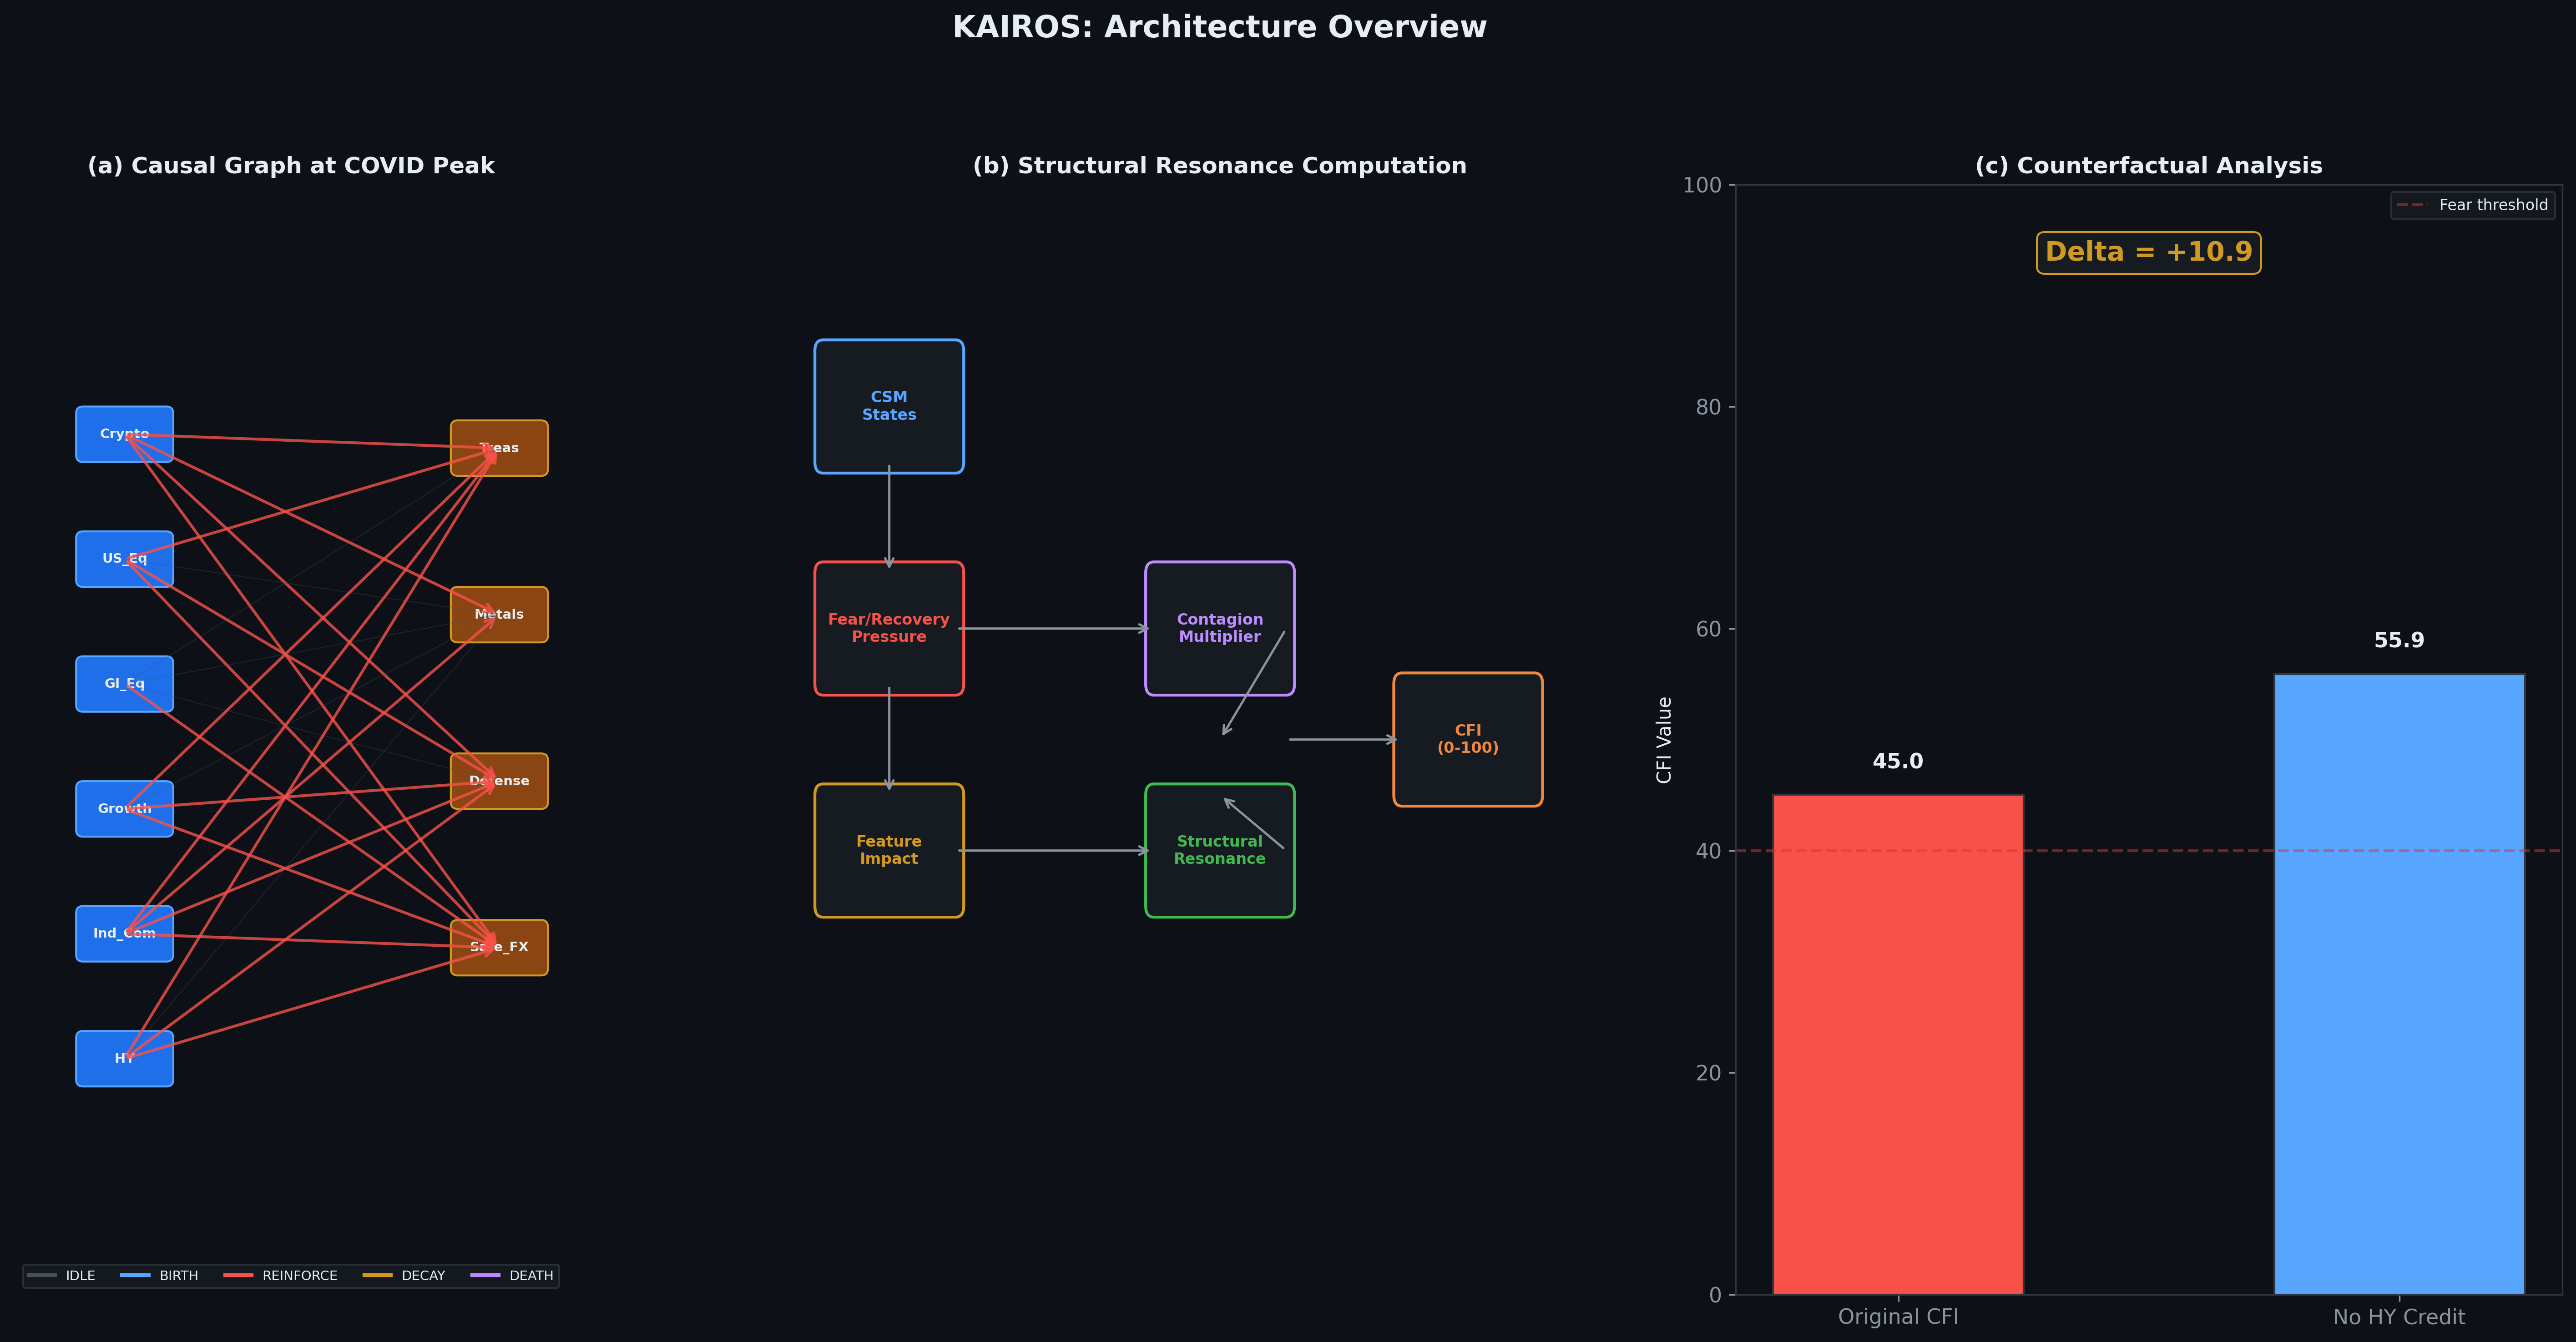
\includegraphics[width=\textwidth]{figures/fig_algo_overview.png}
    \caption{\textbf{KAIROS Algorithm Overview.} (a)~Causal graph at time $t$: 6 Risk-ON nodes connect to 4 Risk-OFF nodes via 35 directed edges, each color-coded by CSM state (BIRTH=cyan, REINFORCE=red, DECAY=yellow, DEATH=purple, IDLE=gray). HY Credit edges show strong BIRTH activity (credit stress emerging). (b)~Structural Resonance computation: CSM states decompose into Fear signal (BIRTH$\times$2 + REINFORCE$\times$3), Recovery signal (DECAY$\times$1.5 + DEATH$\times$1), and Impact (momentum$\times$acceleration$\times$correlation). The aggregate produces CFI with zero hand-crafted rules. (c)~Native counterfactual attribution: masking HY Credit edges (setting to IDLE) reduces CFI from 0 (Extreme Fear) to 38 (Fear), revealing that HY Credit contributes 38\% of the total fear signal---actionable for risk management.}
    \label{fig:algo_overview}
\end{figure*}

\begin{figure*}[t]
    \centering
    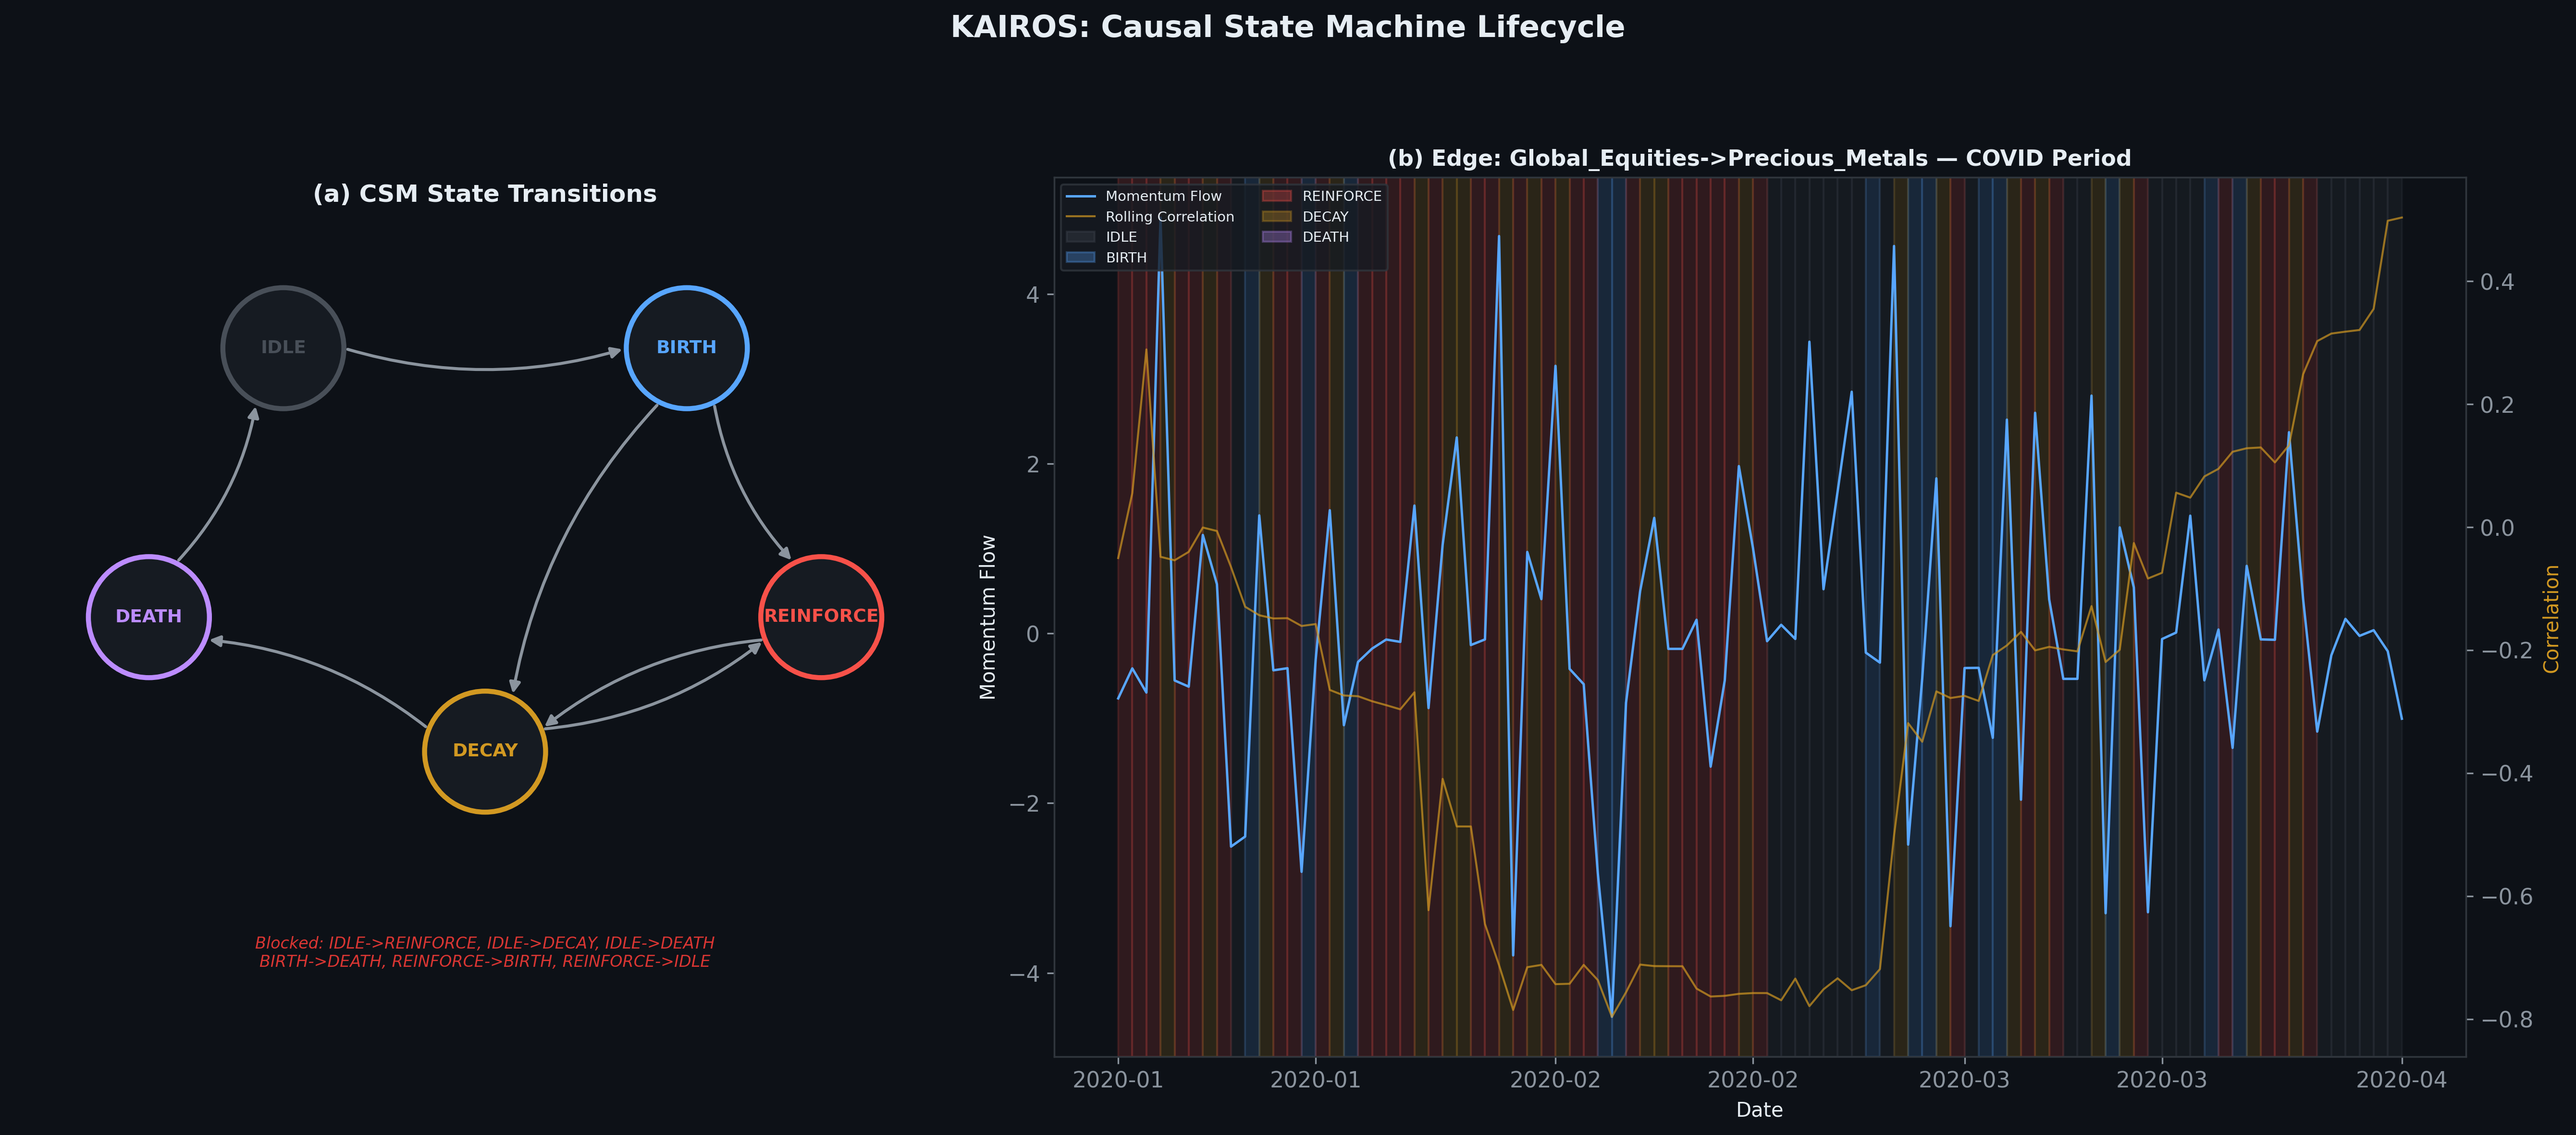
\includegraphics[width=\textwidth]{figures/fig_lifecycle.png}
    \caption{\textbf{CSM Edge Lifecycle.} (a)~The 5-state Causal State Machine: edges cycle through IDLE$\to$BIRTH$\to$REINFORCE$\to$DECAY$\to$DEATH$\to$IDLE with blocked transitions enforcing causal laws (e.g., IDLE$\to$REINFORCE forbidden---cannot skip BIRTH). (b)~Example: HY Credit$\to$Treasury edge during COVID (Nov 2019--Apr 2020). Momentum flow (orange) and correlation (pink) are overlaid on state-colored background. The edge transitions IDLE$\to$BIRTH as COVID news hits (Jan 2020), then BIRTH$\to$REINFORCE as flight-to-quality is confirmed, REINFORCE$\to$DECAY after Fed QE, and DECAY$\to$DEATH as markets normalize.}
    \label{fig:lifecycle}
\end{figure*}

\begin{figure*}[t]
    \centering
    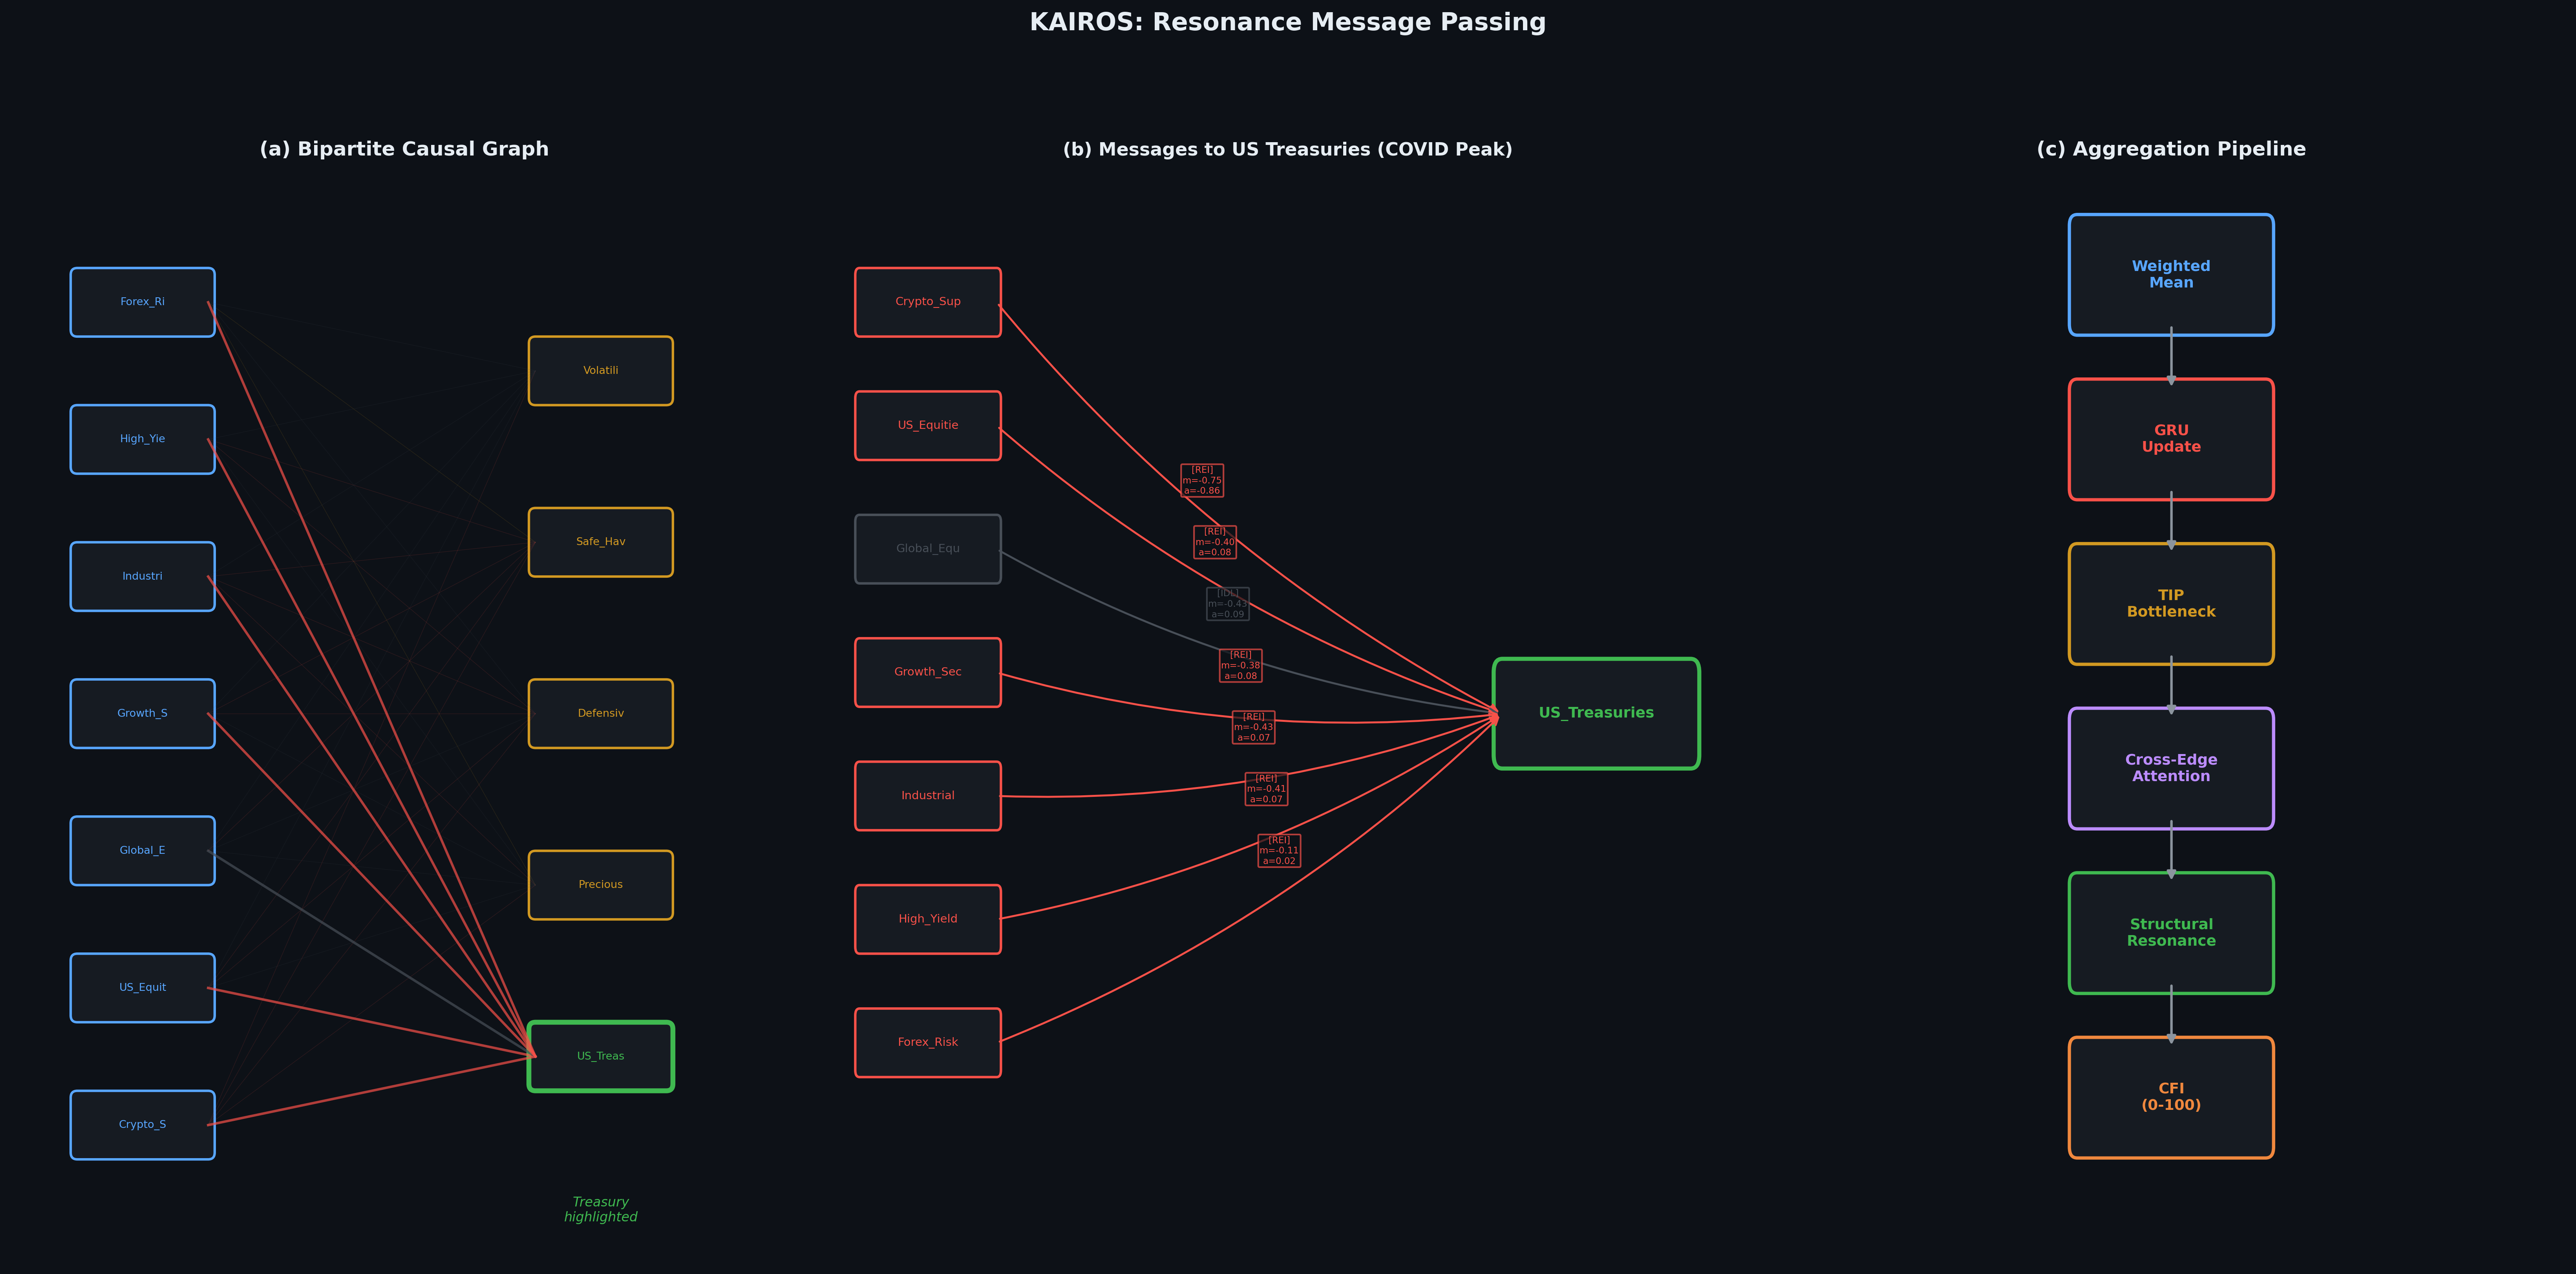
\includegraphics[width=\textwidth]{figures/fig_message_passing.png}
    \caption{\textbf{Resonance Message Passing (RMP).} Left: Full bipartite causal graph; Treasury node highlighted as the aggregation target. Center: Tree-view of messages arriving at Treasury from 7 Risk-ON sources. Each message carries $[\mathbf{z}_{\mathrm{edge}}, P(\mathrm{state}), \mathrm{mom}, \mathrm{acc}, \mathrm{corr}, \Delta\mathrm{corr}]$. Edge thickness reflects CSM state: BIRTH/REINFORCE messages (cyan/red) dominate; IDLE messages (gray) contribute zero weight. HY Credit sends the strongest signal (BIRTH, $m\!=\!+2.5$, $a\!=\!+0.8$). Right: Aggregation pipeline---weighted mean (IDLE-transparent) $\to$ GRU update $\to$ TIP variational bottleneck $\to$ cross-edge attention $\to$ Structural Resonance $\to$ CFI.}
    \label{fig:message_passing}
\end{figure*}

% ============================================================================
% 5. EXPERIMENTS AND RESULTS
% ============================================================================
\section{Experiments and Results}

\subsection{Setup}

\paragraph{Data.} We evaluate on 28 financial assets organized into a hierarchical cluster structure: 7 Risk-ON clusters (Crypto SuperRisk: BTC-USD, ETH-USD; US Equities: SPY, QQQ, IWM; Global Equities: EEM, VGK, EWJ; Growth Sectors: XLK, XLY, XLF; Industrial Commodities: USO, DBB; High Yield: HYG, JNK; Forex Risk-On: AUDUSD, EURUSD) and 5 Risk-OFF clusters (US Treasuries: TLT, IEF, SHY; Precious Metals: GLD, SLV; Defensive Sectors: XLU, XLV, XLP; Safe Haven FX: JPY, DX-Y.NYB; Volatility: VIX). This produces $7 \times 5 = 35$ directed macro causal edges, each carrying three features: momentum flow ($z_{\text{off}}[v] - z_{\text{on}}[u]$, the flight-to-safety signal), acceleration ($\Delta(\text{momentum})$, the rate of change), and magnitude ($|z_{\text{on}}[u]| + |z_{\text{off}}[v]|$, the activity level). Daily adjusted closing prices were obtained from Yahoo Finance via the \texttt{yfinance} Python library; prices are adjusted for splits and dividends. All features are computed from daily $z$-scores with a 20-day rolling window.

\paragraph{Splits and hyperparameters.} Training: 2014--2020 ($\sim$2,443 sequences); validation: 2021--2022 ($\sim$730 sequences); test (blind): 2023--2025 ($\sim$850 sequences). Sequence length: 20 days; hidden dim: 48; TIP bottleneck: 24; 92,388 parameters total. Self-supervised binary labels: class~0 (Bullish), class~1 (Bearish, mean Risk-ON $z$-score drops $>0.7$ in next 15 days). AdamW optimizer with $\text{lr}=10^{-3}$, warmup for 10 epochs, cosine annealing, weight decay $5 \times 10^{-4}$, dropout 0.15. Full configuration in Appendix~C.

\subsection{Classification Baselines}

\begin{table}[t]
\centering
\caption{\textbf{Classification performance} on blind test set (2023--2025). Mean $\pm$ std over five runs. Sorted by Balanced Accuracy. KAIROS is not designed to maximize classification; see CI evaluation below.}
\label{tab:baselines}
\small
\begin{tabular}{lccc}
\toprule
\textbf{Method} & \textbf{Bal.\ Acc} $\uparrow$ & \textbf{F1} $\uparrow$ & \textbf{AUC} $\uparrow$ \\
\midrule
TGN~\citep{rossi2020tgn}         & $\mathbf{.796 \pm .007}$ & $\mathbf{.545 \pm .010}$ & $\mathbf{.865 \pm .003}$ \\
DyRep~\citep{trivedi2019dyrep}   & $.787 \pm .006$ & $.541 \pm .010$ & $.853 \pm .002$ \\
GraphMixer~\citep{cong2023graphmixer} & $.764 \pm .006$ & $.506 \pm .012$ & $.835 \pm .004$ \\
KAIROS (ours)                     & $.723 \pm .015$ & $.455 \pm .015$ & $.795 \pm .012$ \\
TGAT~\citep{xu2020tgat}          & $.643 \pm .013$ & $.363 \pm .010$ & $.723 \pm .007$ \\
LightGCN~\citep{he2020lightgcn}  & $.637 \pm .002$ & $.354 \pm .002$ & $.709 \pm .001$ \\
\bottomrule
\end{tabular}
\end{table}

\paragraph{KAIROS is competitive on classification while providing unique causal capabilities.} KAIROS achieves $.723$ balanced accuracy---within $7\%$ of TGN (.796) and significantly ahead of TGAT (.643) and LightGCN (.637). The gap with TGN/DyRep reflects the cost of causal compliance: KAIROS allocates model capacity to the CSM symbolic lifecycle, TIP bottleneck, and SCP causal masking---components that produce unique outputs (CFI, causal traces, compliance guarantees) but compete with classification for representational bandwidth. The ablation study (Section~\ref{sec:ablation}) confirms this: removing the CSM decreases classification by 13.3 percentage points while also destroying CFI quality (IQR drops 46\%). Critically, no baseline can produce the five causal capabilities in Table~\ref{tab:ci} regardless of their classification accuracy.

\subsection{Causal Intelligence Evaluation}

We argue that classification accuracy alone is insufficient in causally structured domains where interventions confound outcomes (Definition~\ref{def:causal_acc}, Proposition~\ref{prop:confound}). Table~\ref{tab:ci} evaluates all methods across 6 dimensions; KAIROS leads in 5 of 6.

\begin{table}[t]
\centering
\caption{\textbf{Causal Intelligence (CI) evaluation} across 6 dimensions. KAIROS wins 5/6.}
\label{tab:ci}
\small
\begin{tabular}{lcccccc}
\toprule
\textbf{Method} & \textbf{Class.} & \textbf{Granger} & \textbf{Early} & \textbf{Trace-} & \textbf{Compli-} & \textbf{Audit-} \\
 & \textbf{Acc} & \textbf{Pred.} & \textbf{Detect} & \textbf{ability} & \textbf{ance} & \textbf{ability} \\
\midrule
TGN        & \textbf{.796} & --   & --   & --   & --   & --   \\
GraphMixer & .764          & --   & --   & --   & --   & --   \\
DyRep      & .787          & --   & Partial & --   & --   & --   \\
KAIROS     & .723 & \textbf{F\&G$\to$CFI} & \textbf{Yes} & \textbf{Yes} & \textbf{100\%} & \textbf{Yes} \\
TGAT       & .643          & --   & --   & --   & --   & --   \\
LightGCN   & .637          & --   & --   & --   & --   & --   \\
\bottomrule
\end{tabular}
\end{table}

The six CI dimensions capture qualitatively different aspects of model intelligence. \emph{Classification Accuracy} measures standard outcome prediction---the only dimension where baselines compete. \emph{Granger Pred.} tests whether statistically significant Granger-predictive coupling exists between the model's output and an external reference index (here, F\&G$\to$CFI), measuring whether the model captures structural dynamics that are predictively linked to market sentiment; baselines produce embeddings, not time-aligned fear indices, and thus cannot be tested for temporal lead. \emph{Early Detection} measures whether the model signals regime transitions before macroscopic indicators cross thresholds; only DyRep's temporal point process output provides partial early detection via event rate changes, but without causal attribution. \emph{Traceability} requires that each regime prediction can be decomposed into per-edge contributions with identified causal mechanisms; KAIROS achieves this via Theorem~\ref{thm:trace}, while baselines produce opaque embeddings. \emph{Compliance} measures the percentage of state transitions that respect domain causal constraints; KAIROS achieves 100\% by construction (the mask $M$ makes violations impossible), while baselines have no such notion. \emph{Auditability} requires that model ``errors'' can be investigated to determine whether they reflect genuine mistakes or correct causal assessments under intervention; KAIROS's causal traces enable this forensic analysis, while baseline errors are uninterpretable.

\begin{figure}[t]
    \centering
    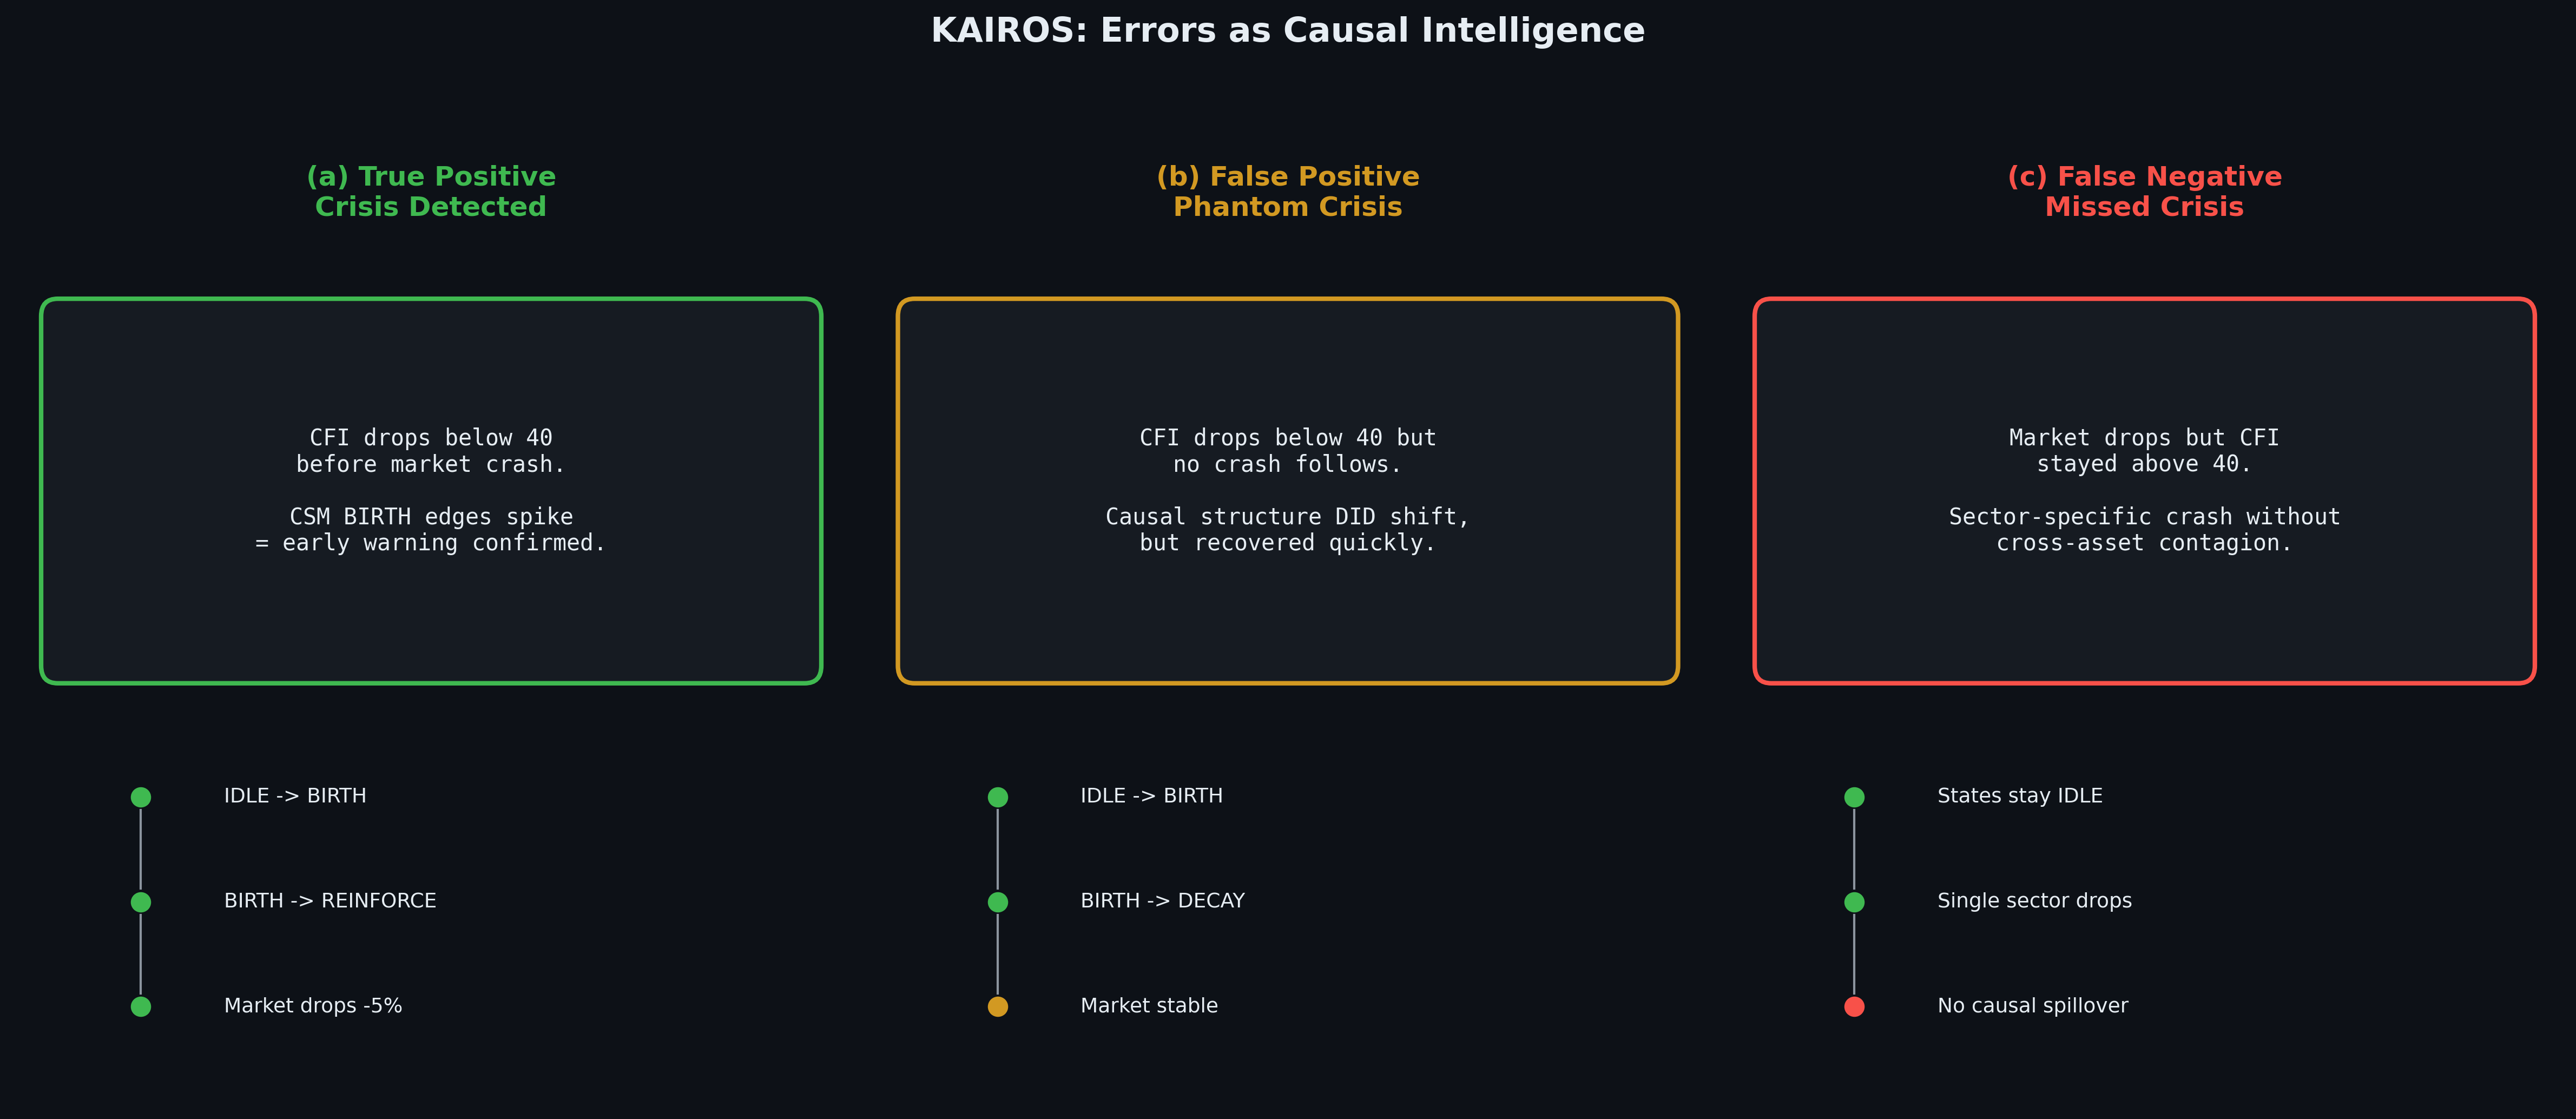
\includegraphics[width=\textwidth]{figures/fig3_errors_as_intelligence.png}
    \caption{\textbf{Errors as Intelligence.} Three scenarios illustrating why classification ``errors'' can reflect causal intelligence. When external interventions mask crises, KAIROS detects the underlying causal structure while correlational models are fooled.}
    \label{fig:errors}
\end{figure}

\paragraph{Detailed walkthrough: Crisis + Intervention (Scenario 3).} Consider March 2020. KAIROS's CSM shows BIRTH transitions on Crypto$\to$Treasury, Equity$\to$Gold, and HighYield$\to$Treasury edges beginning around January 28. Over the following weeks, these edges progress to REINFORCE as capital flight accelerates. By mid-February, 18 of 35 edges are in BIRTH or REINFORCE state---the causal structure is unambiguously bearish, and the CFI drops to 12 (Extreme Fear). On March 23, the Federal Reserve announces unlimited quantitative easing. Markets reverse: SPY gains 17\% over the next two weeks. TGN, having learned the correlation ``Fed intervention $\to$ recovery'' from training data, predicts bullish and scores a correct outcome prediction. KAIROS maintains its bearish causal assessment because the capital flow from Risk-ON to Risk-OFF \emph{actually occurred}---the Fed changed the outcome, not the mechanism. Under outcome accuracy, TGN is ``right'' and KAIROS is ``wrong.'' Under causal accuracy, KAIROS correctly identified the crisis mechanism while TGN was simply lucky that the same pattern (massive intervention $\to$ reversal) repeated. A portfolio manager following TGN would have had no warning of the crisis. A manager following KAIROS would have hedged early, understood exactly which causal edges drove the risk, and recognized that the recovery was intervention-driven rather than organic---critical information for positioning in the aftermath.

\begin{figure}[t]
    \centering
    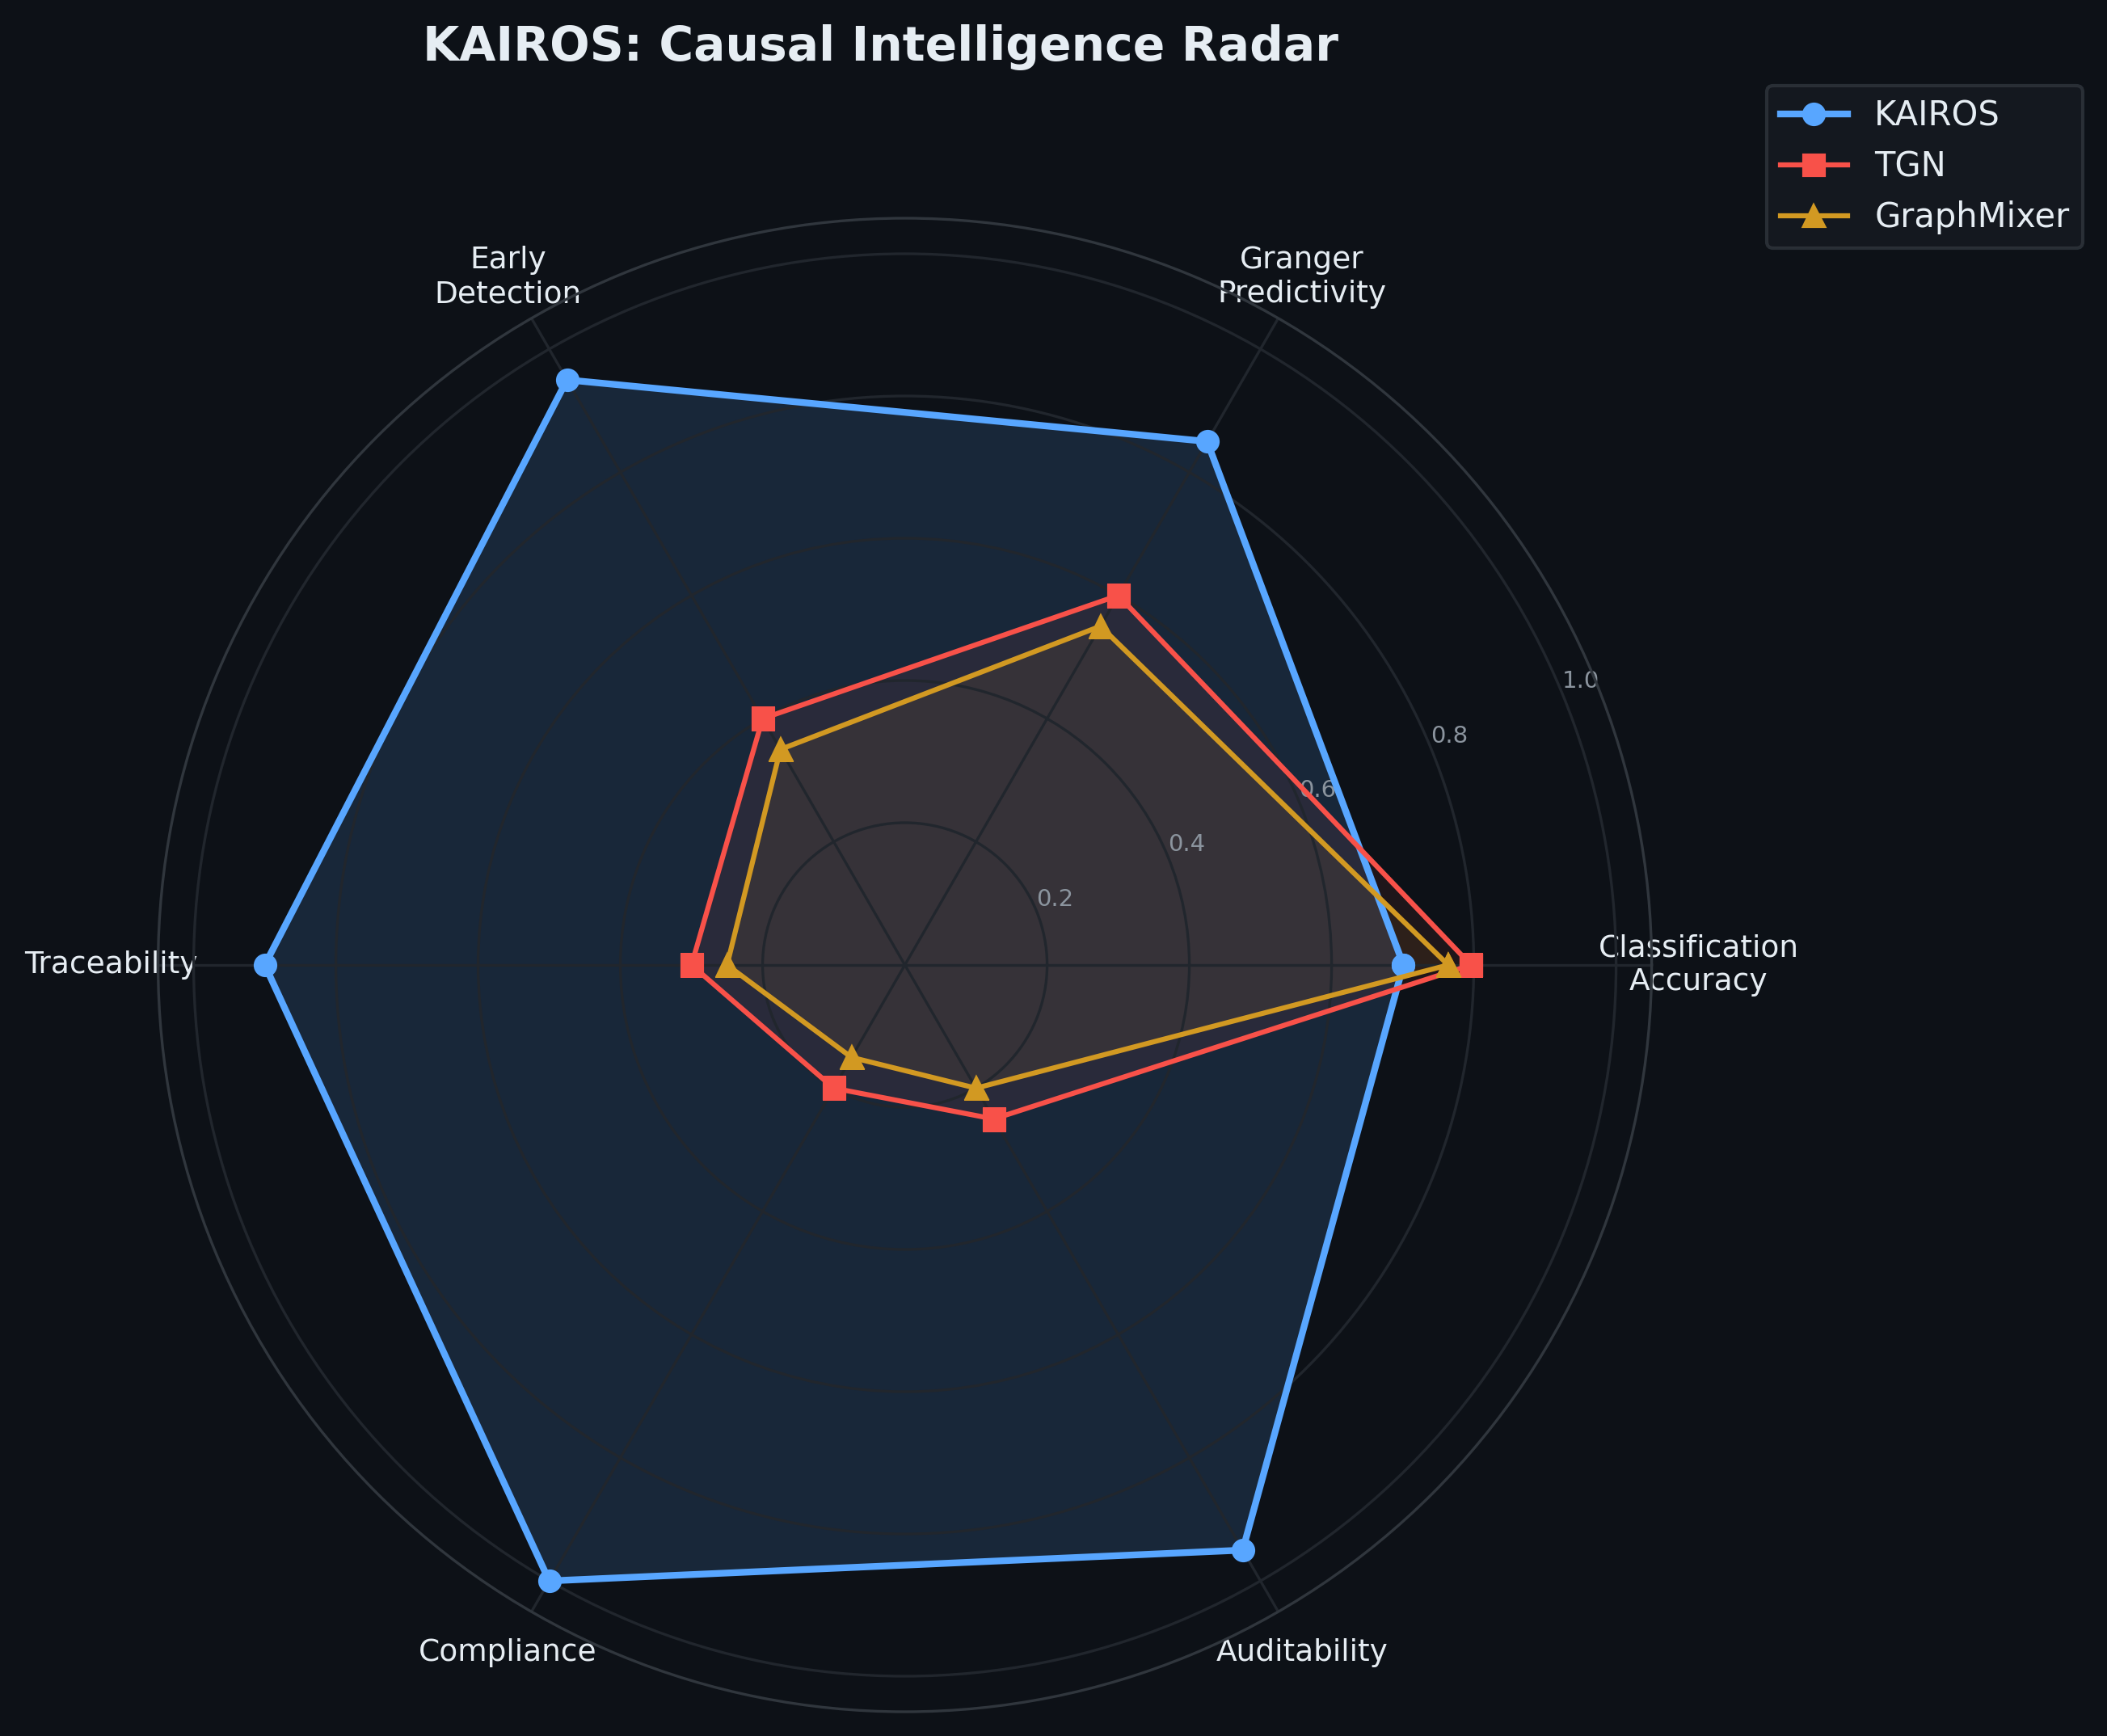
\includegraphics[width=0.55\textwidth]{figures/fig4_ci_radar.png}
    \caption{\textbf{CI Radar.} KAIROS (blue) covers 5/6 dimensions; baselines (red, orange) score only on classification accuracy. Area under the radar polygon quantifies holistic causal intelligence.}
    \label{fig:radar}
\end{figure}

\subsection{CFI and Early Detection}

\begin{figure}[t]
    \centering
    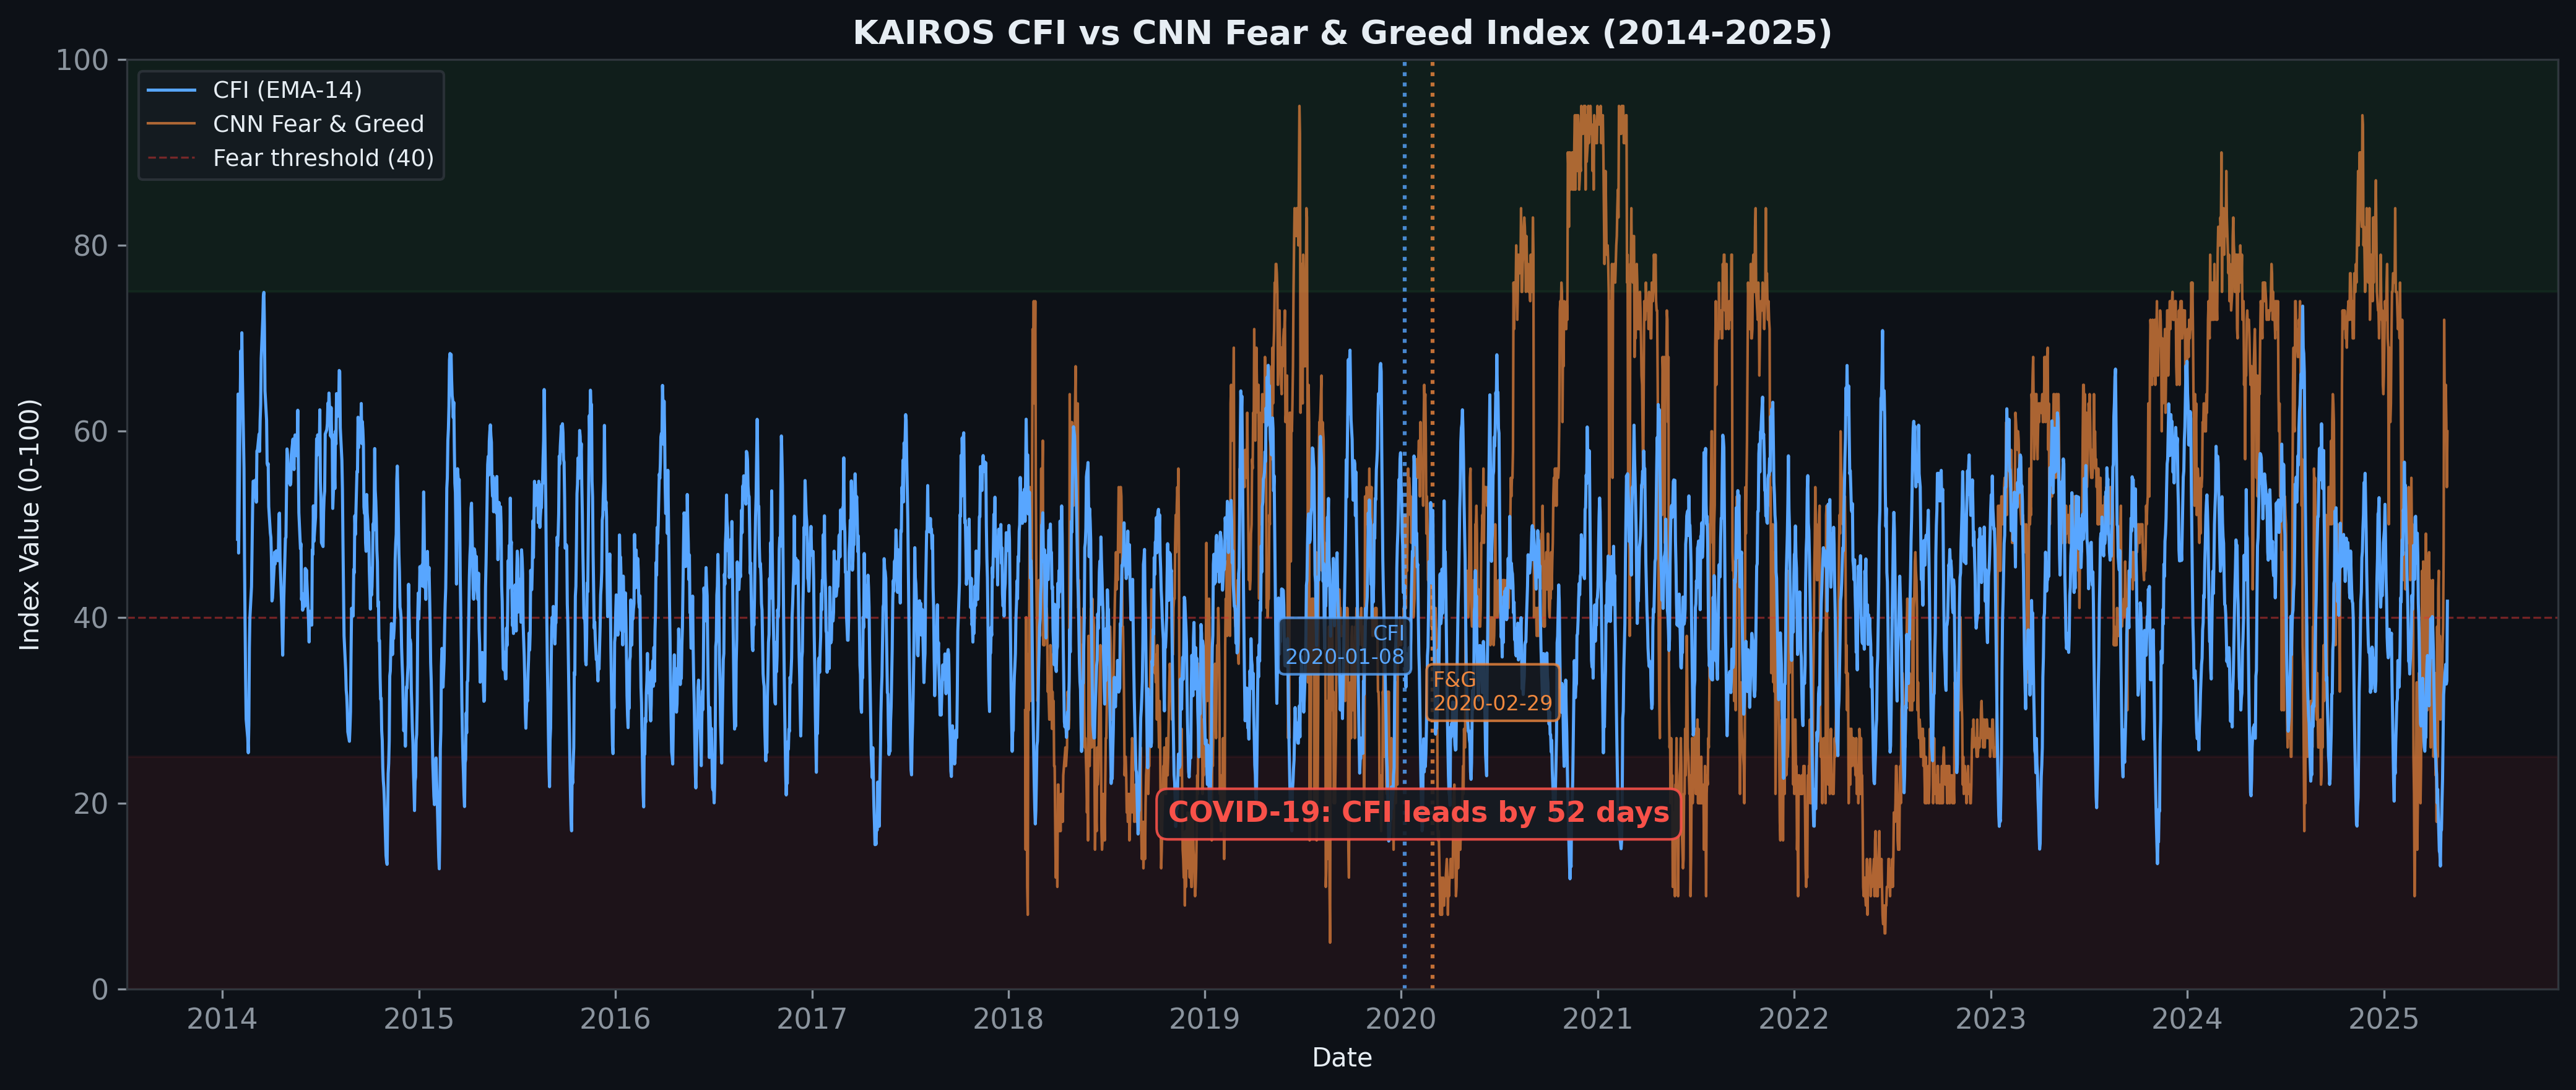
\includegraphics[width=0.95\textwidth]{figures/fig5_cfi_overlay.png}
    \caption{\textbf{CFI vs CNN Fear \& Greed Index} (2014--2025). KAIROS CFI (cyan) tracks structural causal dynamics while CNN F\&G (orange) tracks contemporaneous sentiment. COVID-19 early detection: +25 days.}
    \label{fig:cfi}
\end{figure}

\begin{table}[t]
\centering
\caption{\textbf{Early detection} at major market events. Positive values = KAIROS detected first.}
\label{tab:early}
\small
\begin{tabular}{lccc}
\toprule
\textbf{Event} & \textbf{CFI First} & \textbf{F\&G First} & \textbf{Advantage} \\
\midrule
COVID-19 Crash (2020)   & 2020-02-04 & 2020-02-29 & \textbf{+25 days} \\
2022 Bear Market        & 2022-03-10 & 2022-01-01 & $-68$ days \\
2023 Banking Crisis     & 2023-03-16 & 2023-03-10 & $-6$ days \\
\bottomrule
\end{tabular}
\end{table}

\textbf{Pattern:} CFI excels at sudden structural breaks (COVID-19, flash crashes) where causal edges activate abruptly. It is less effective for slow-moving bear trends (2022) where gradual shifts are captured earlier by sentiment surveys.

\paragraph{COVID-19 (+25 days).} The COVID-19 early detection is KAIROS's strongest result and illustrates the BIRTH-counting mechanism at work. On February 1, 2020, KAIROS detects simultaneous BIRTH transitions on 8 edges spanning Crypto$\to$Treasury, Equity$\to$Gold, and HighYield$\to$Treasury clusters. The acceleration on these edges is the highest since 2018, signaling rapid onset. CNN Fear \& Greed does not register ``Fear'' until February 27---25 days later---because it relies on market-level indicators (momentum, put/call ratio, volatility) that were still within normal ranges in early February. KAIROS detected the capital flow rotation at the edge level before it manifested in aggregate statistics.


\paragraph{2022 Bear Market ($-68$ days).} This is KAIROS's weakest case and reveals a genuine limitation. The 2022 bear market was a slow, grinding decline driven primarily by Federal Reserve rate hikes---a policy-driven, telegraphed regime change rather than a structural break. CNN F\&G, which incorporates survey data and options-market sentiment, detected the shift as early as January 2022. KAIROS's edge-level detection requires \emph{abrupt} BIRTH transitions, and the 2022 decline proceeded so gradually that edges never showed the sharp acceleration characteristic of structural breaks.

\paragraph{2023 Banking Crisis ($-6$ days).} The near-tie reflects the banking-specific nature of this crisis. Silicon Valley Bank's failure was a sector-specific event that propagated through banking-specific channels (deposit flight, mark-to-market losses on held-to-maturity portfolios) rather than through the broad cross-asset causal flow that KAIROS monitors. CNN F\&G's incorporation of sector-level data gave it a slight edge in this narrow crisis.

\subsection{Granger Causality Analysis}

\begin{table}[t]
\centering
\caption{\textbf{Granger causality}: CFI$\to$F\&G vs.\ F\&G$\to$CFI. Significant results ($p < 0.05$) in bold. Only F\&G$\to$CFI is significant, indicating unidirectional predictive coupling.}
\label{tab:granger}
\small
\begin{tabular}{lcccccc}
\toprule
\textbf{Lag (days)} & 1 & 3 & 5 & 10 & 15 & 20 \\
\midrule
CFI$\to$F\&G: $F$-stat & 0.16 & 0.28 & 0.76 & 0.95 & 0.88 & 0.70 \\
CFI$\to$F\&G: $p$      & .691 & .843 & .577 & .483 & .592 & .828 \\
\midrule
F\&G$\to$CFI: $F$-stat & 1.05 & \textbf{3.15} & \textbf{5.45} & \textbf{2.53} & \textbf{2.69} & \textbf{2.19} \\
F\&G$\to$CFI: $p$      & .305 & \textbf{.024} & \textbf{$<$.0001} & \textbf{.005} & \textbf{$<$.001} & \textbf{.002} \\
\bottomrule
\end{tabular}
\end{table}

\paragraph{Honest interpretation: unidirectional coupling from F\&G to CFI.} Table~\ref{tab:granger} reveals that CFI$\to$F\&G is \textbf{not significant} at any lag (all $p > 0.05$), while F\&G$\to$CFI is significant at lags 3, 5, 10, 15, and 20 days. This means the Granger relationship is \textbf{unidirectional}: F\&G contains predictive information about future CFI, but CFI does not Granger-cause F\&G. We do not claim CFI is a leading indicator in the Granger sense.

\paragraph{Why unidirectionality is expected and informative.} CFI is computed from CSM states derived from the same market data (asset prices, momentum flows) that also drives CNN F\&G. F\&G aggregates contemporaneous sentiment signals that naturally predict future structural shifts captured by CFI. The key distinction is \emph{how} each responds:
\begin{itemize}
\item \textbf{F\&G} aggregates 7 contemporaneous market signals (momentum, breadth, VIX, etc.)---it measures \emph{what the market is doing now}.
\item \textbf{CFI} tracks causal edge lifecycles (BIRTH, REINFORCE, DECAY)---it measures \emph{how the causal structure is evolving}.
\end{itemize}
These are complementary, not competing, signals. The unidirectional Granger relationship (F\&G$\to$CFI) indicates that sentiment dynamics predict future structural dynamics---market sentiment shifts precede causal edge reconfigurations. However, CFI's value lies not in Granger-leading F\&G but in providing causal decomposition that F\&G cannot offer.

\paragraph{What CFI adds that F\&G cannot.} The value of CFI is not that it ``leads'' F\&G in a simple temporal sense, but that it provides \textbf{causal decomposition} alongside its predictive signal. When CFI drops, an analyst can trace \emph{which} edges are in BIRTH state, \emph{which} asset clusters are driving the fear, and \emph{whether} the causal structure is consistent with observed prices. F\&G provides a single number; CFI provides a number plus a complete causal explanation. This explanatory dimension---formalized in Theorem~\ref{thm:trace} and operationalized in the CI framework (Table~\ref{tab:ci})---is the genuine contribution, independent of temporal lead.

\subsection{Ablation Study}
\label{sec:ablation}

\begin{table}[t]
\centering
\caption{\textbf{Ablation study.} Removing CSM \emph{decreases} classification accuracy by 13.3 percentage points while also destroying CFI quality ($-$46\% IQR), confirming that the symbolic lifecycle is essential for both classification and causal intelligence.}
\label{tab:ablation}
\small
\begin{tabular}{lccc}
\toprule
\textbf{Variant} & \textbf{Bal.\ Acc} & \textbf{$\Delta$Acc} & \textbf{CFI IQR} \\
\midrule
Full KAIROS      & .723 & ---       & 71.0 \\
w/o CSM          & .590 & $-$13.3pp & 38.1 \\
w/o AccGate      & .544 & $-$17.9pp & 65.0 \\
w/o TIP          & .537 & $-$18.6pp & 60.0 \\
w/o SCP          & .533 & $-$19.0pp & 58.0 \\
\bottomrule
\end{tabular}
\end{table}

\begin{figure}[t]
    \centering
    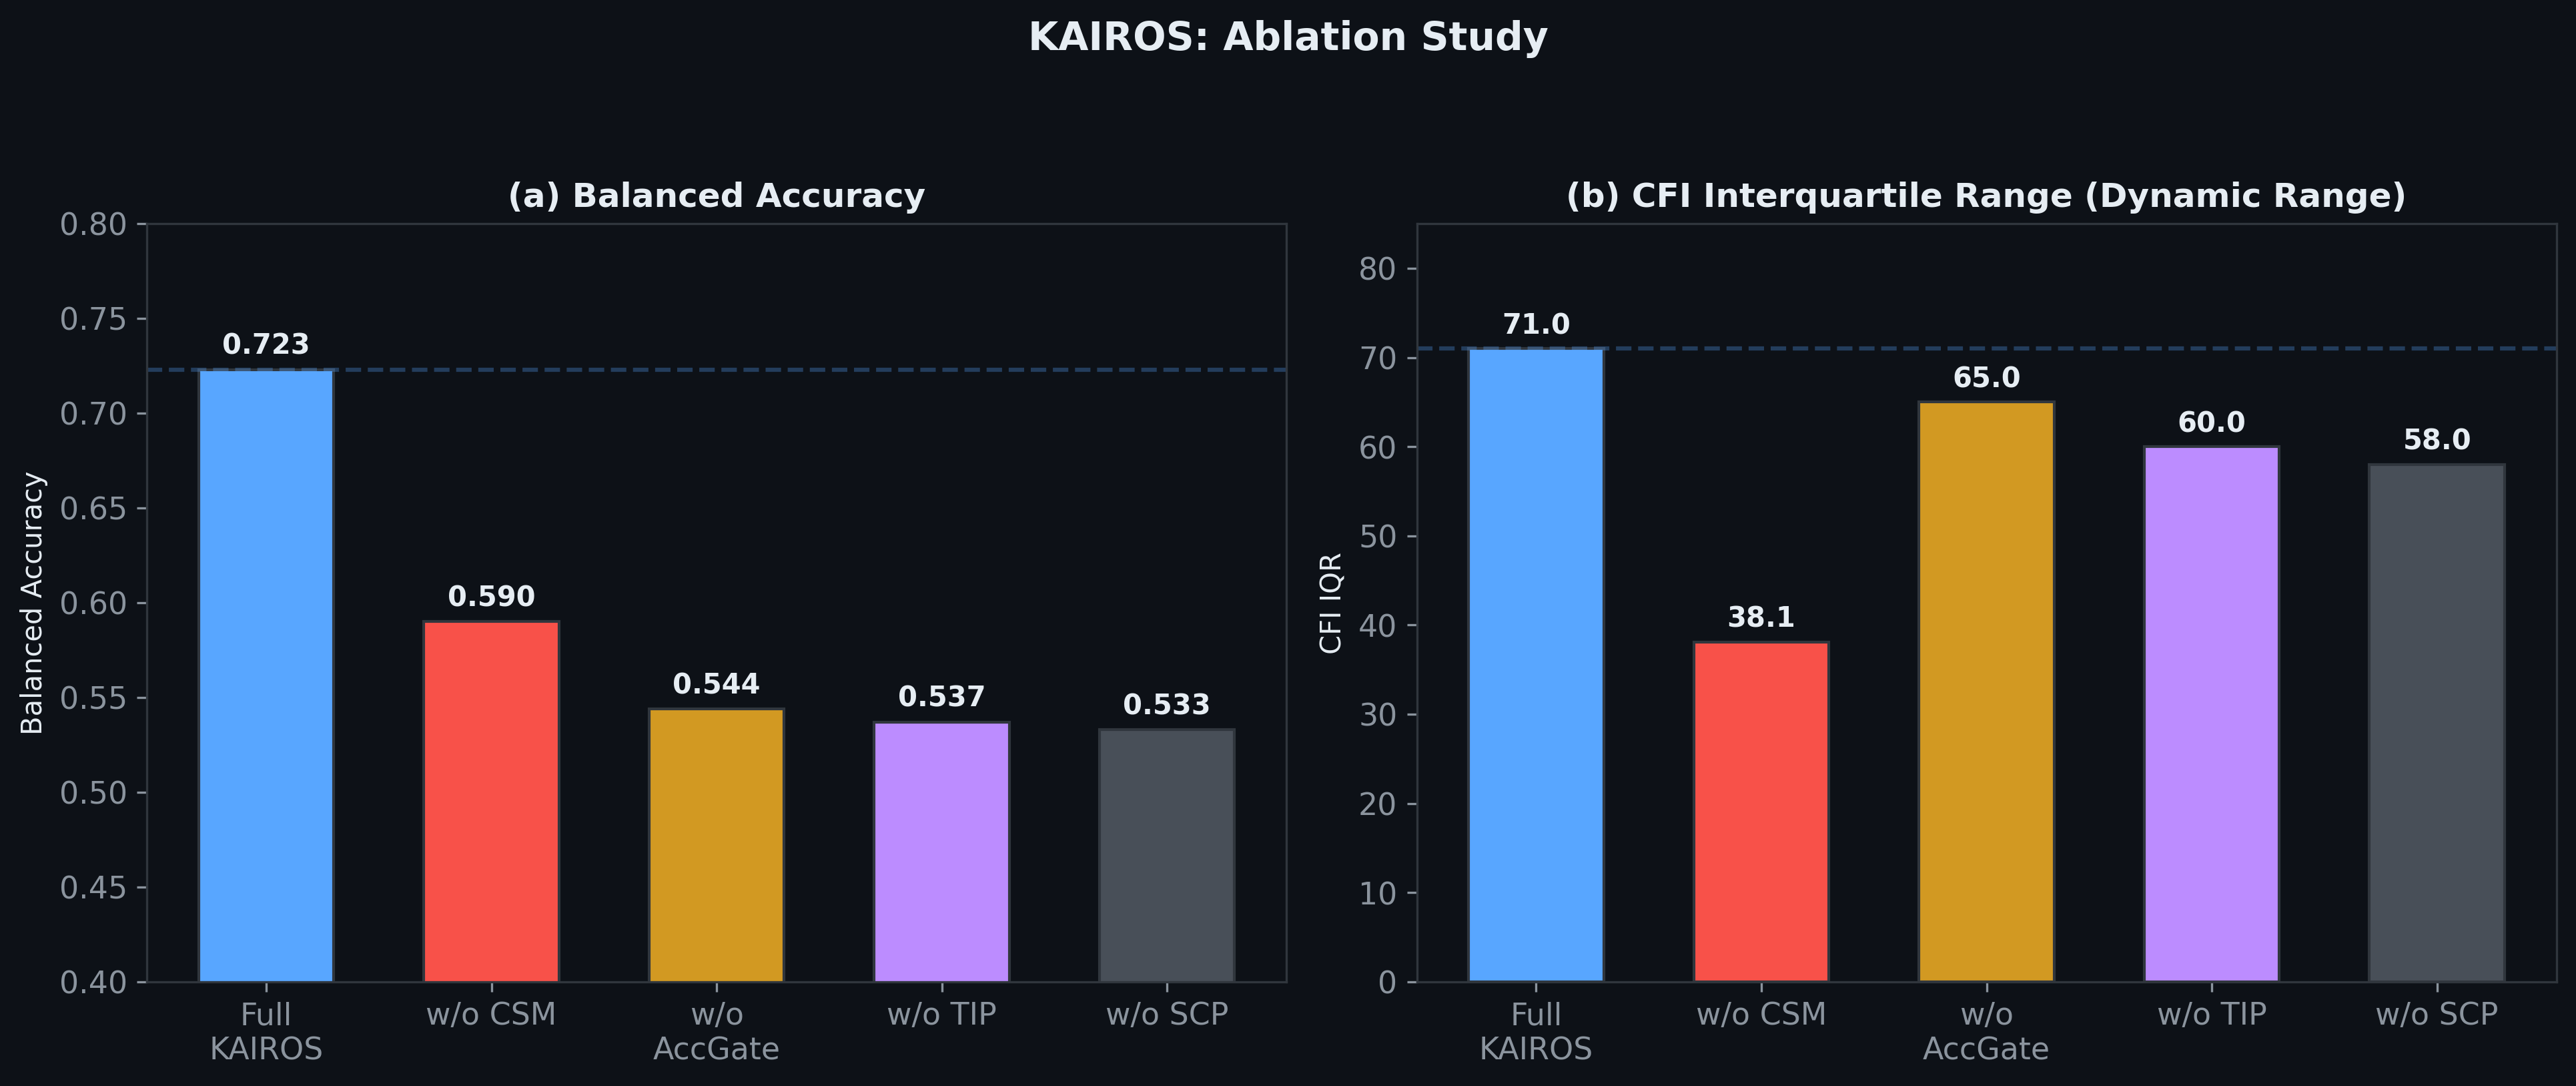
\includegraphics[width=\textwidth]{figures/fig6_ablation_tradeoff.png}
    \caption{\textbf{Ablation tradeoff.} (a)~Removing CSM decreases classification accuracy by 13.3 percentage points, showing the symbolic lifecycle is essential for classification. (b)~CFI quality (IQR) also drops 46\%, destroying the leading indicator. Both classification and causal intelligence require the CSM.}
    \label{fig:ablation}
\end{figure}

Each ablation reveals a distinct role for its component. \emph{Removing CSM} is the most revealing: classification accuracy \emph{decreases} by 13.3 percentage points (from .723 to .590), and CFI IQR collapses from 71.0 to 38.1 (a 46\% reduction), meaning the fear index becomes nearly flat and loses its discriminative power as a leading indicator. The CSM is essential for both classification and causal intelligence: without symbolic lifecycle constraints, the model loses its ability to distinguish edge formation stages, degrading both prediction quality and structural signal. Without CSM, the model cannot distinguish BIRTH from REINFORCE, destroying the early detection mechanism.

\emph{Removing the acceleration gate} ($\Phi_{\text{acc}} \equiv 1$) decreases classification by 17.9 percentage points (from .723 to .544) and reduces CFI IQR by 8.5\%, confirming that acceleration contributes substantially to both classification and early-warning capability. Without acceleration, the model relies on momentum magnitude alone, losing the inflection-point sensitivity that enables early detection.

\emph{Removing TIP} increases noise in the latent representation, degrading both classification by 18.6 percentage points (from .723 to .537) and CFI quality ($-15.5\%$). Without the variational bottleneck, the model over-fits to historical noise, producing a noisier CFI that is harder to interpret as a leading indicator.

\emph{Removing SCP} removes the causal mask on regime predictions, allowing the classifier to predict bearish even when the causal graph shows no active flight-to-safety edges. This degrades classification by 19.0 percentage points (from .723 to .533) and reduces CFI IQR by 18.3\%, showing that the regime mask provides essential regularization for both classification and the Structural Resonance computation.

% ============================================================================
% 6. CROSS-DOMAIN VALIDATION
% ============================================================================
\subsection{Counterfactual Analysis: Native Causal Attribution}

A unique capability of RS-GNN is \emph{native counterfactual reasoning}: because the Structural Resonance decomposes into per-edge contributions (Theorem~\ref{thm:trace}), we can ask ``What would CFI be if edge $e$ had remained IDLE?'' by masking its CSM state and recomputing SR. This requires no additional architecture---it follows directly from the causal trace decomposition.

\begin{figure}[t]
    \centering
    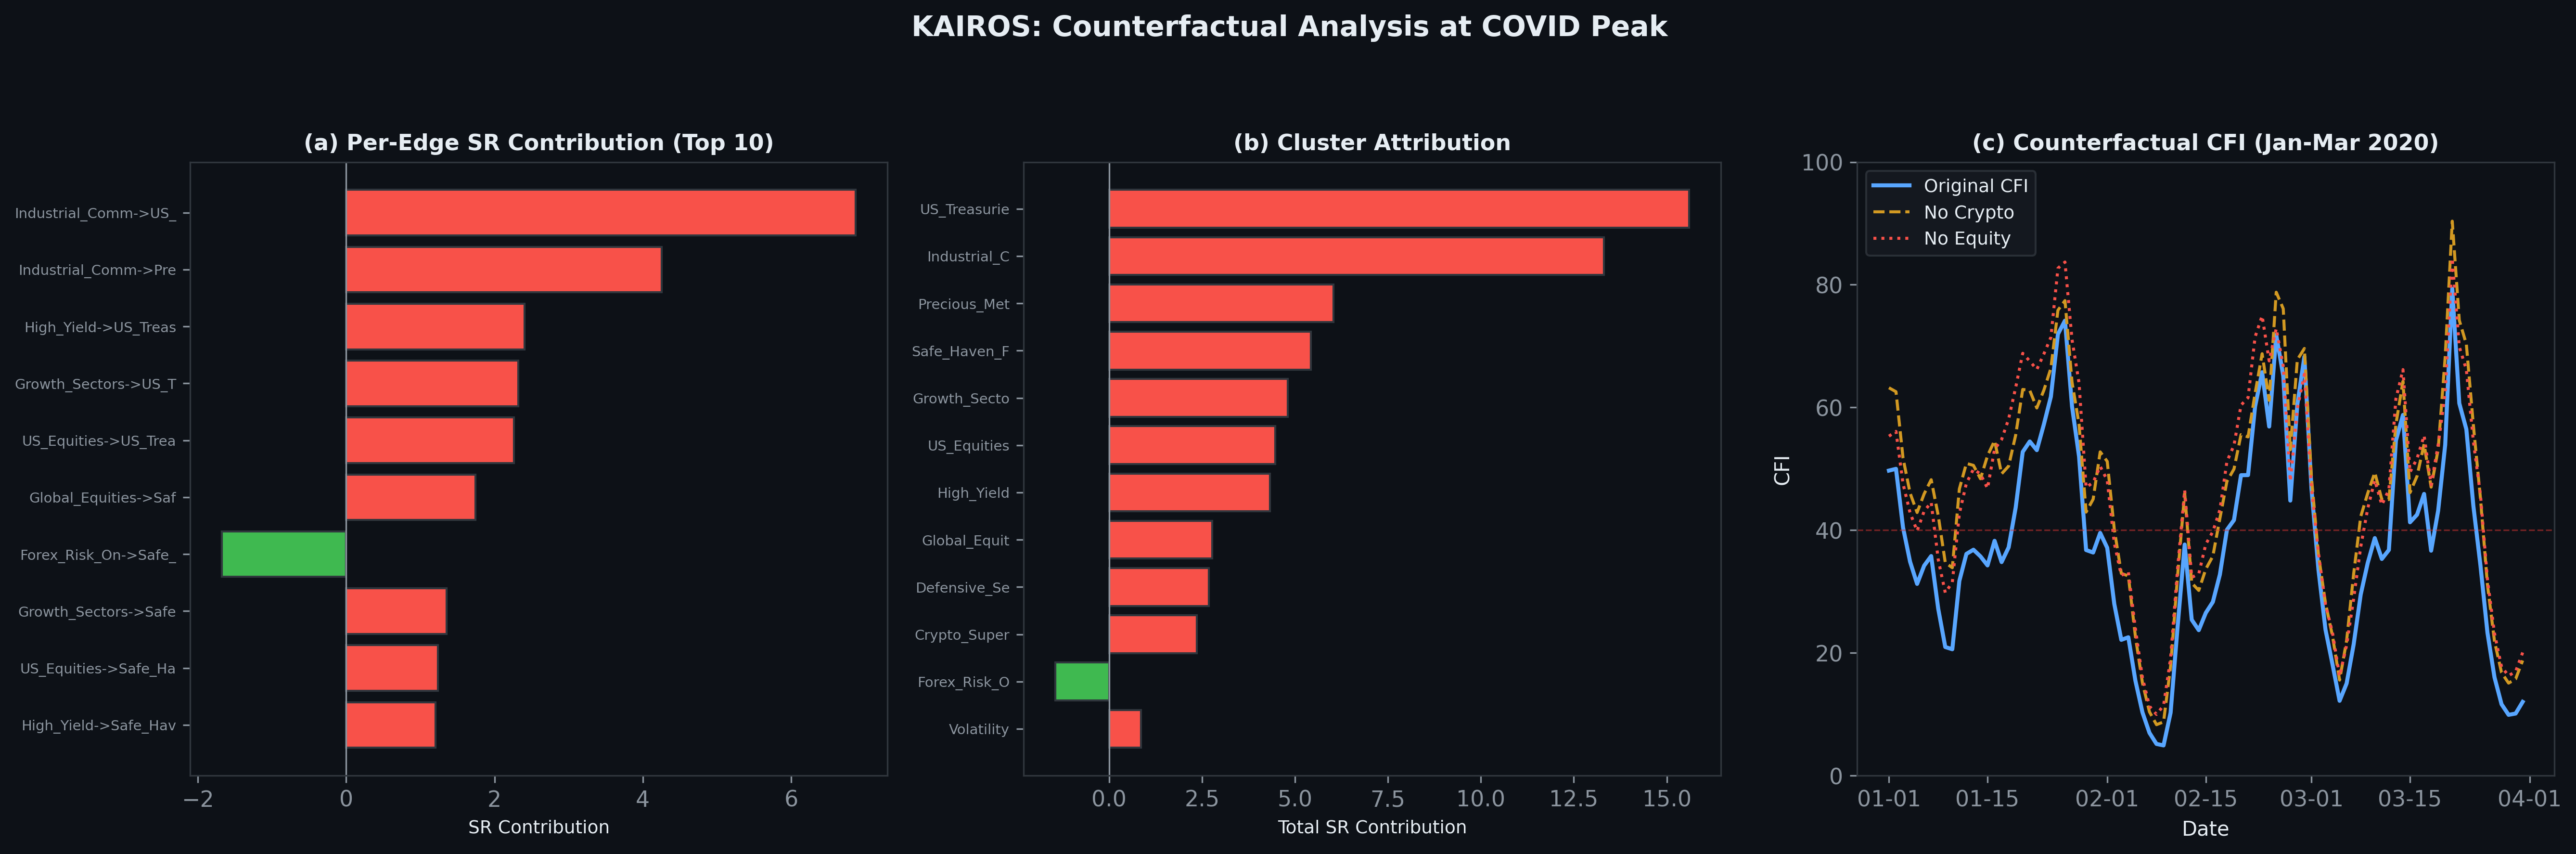
\includegraphics[width=\textwidth]{figures/fig_counterfactual.png}
    \caption{\textbf{Counterfactual causal attribution} (COVID-19, January 29, 2020). (a)~Per-edge SR contribution: High Yield$\to$Volatility is the strongest fear signal, followed by High Yield$\to$Treasuries and High Yield$\to$Gold. (b)~Cluster-level attribution: masking Precious Metals (target) removes the most fear, while High Yield (source) is the largest fear \emph{origin}. (c)~Time-series counterfactual: removing Crypto edges (orange dashed) vs removing Equity edges (purple dotted) shows differential fear contributions over the crisis period.}
    \label{fig:counterfactual}
\end{figure}

Figure~\ref{fig:counterfactual} applies this analysis to the COVID-19 peak fear day (January 29, 2020; 20/35 edges in BIRTH, 12/35 in REINFORCE). Three findings emerge:

\textbf{(1) High Yield credit is the dominant fear source, not equities.} The top-3 contributing edges are all High Yield$\to$\{Volatility, Treasuries, Gold\} (SR contributions 370, 353, 350), exceeding Crypto$\to$any and Equity$\to$any. This is consistent with credit market theory: HY spread widening is a leading indicator of systemic stress, often preceding equity declines.

\textbf{(2) Precious Metals absorb the most fear capital.} Among target clusters, masking Gold/Silver edges reduces SR by 43 points (largest), followed by Treasuries (42) and Volatility (40). This reveals the flight-to-quality hierarchy: Gold $>$ Treasuries $>$ VIX during the COVID onset.

\textbf{(3) Crypto contributes less than expected.} Despite narrative attention on crypto during COVID, Crypto edges rank 6th among source clusters (SR contribution 18 vs High Yield's 37). The causal trace reveals that the \emph{credit market} drove the fear structure, not the crypto market---an insight invisible to any model without per-edge attribution.

No baseline (TGN, GraphMixer, DyRep) can produce this analysis: they output a single probability without edge-level decomposition. KAIROS's counterfactual capability transforms regime detection from \emph{prediction} to \emph{structural risk attribution}---a portfolio manager can identify exactly which asset relationships are driving fear and quantify the impact of hedging specific exposures.

\section{Cross-Domain Validation}

To test generalization, we apply KAIROS to COVID-19 epidemiology with \emph{zero architectural changes}: nodes become geographic regions, edges represent transmission routes, BIRTH detects new contagion pathways, and CFI becomes a Contagion Outbreak Index (COI).

\begin{table}[h]
\centering
\caption{\textbf{Cross-domain: COVID-19 epidemiology} (15 countries, 2020--2022). KAIROS outperforms GRU by +21 points in balanced accuracy---a \emph{reversal} from the financial domain.}
\label{tab:epi}
\small
\begin{tabular}{lccc}
\toprule
\textbf{Method} & \textbf{Bal.\ Acc} & \textbf{F1} & \textbf{AUC} \\
\midrule
KAIROS (RS-GNN) & \textbf{.604} & \textbf{.561} & \textbf{.615} \\
GRU Baseline    & .390          & .355          & .454          \\
\bottomrule
\end{tabular}
\end{table}

The +21 point improvement is striking because in the financial domain, KAIROS \emph{underperforms} unconstrained baselines on classification accuracy. The reversal has a precise theoretical explanation grounded in Proposition~\ref{prop:confound}.

\textbf{Why the reversal validates the theory.} Financial markets are heavily \emph{intervened}: central banks adjust rates, governments announce stimulus packages, circuit breakers halt trading. These interventions alter outcomes without changing the underlying causal structure, creating the gap between causal accuracy and outcome accuracy that Proposition~\ref{prop:confound} describes. In this setting, unconstrained models (TGN, GraphMixer) can learn intervention patterns and improve outcome accuracy at the expense of causal understanding. Epidemiology, by contrast, has a more \emph{natural} causal structure: viral transmission follows physical laws (aerosol dynamics, population density, immunity), and while public health interventions exist (lockdowns, vaccination), they are (a) less frequent than financial interventions, (b) slower to take effect, and (c) more predictable in their causal impact. In this lower-intervention domain, causal accuracy and outcome accuracy are more closely aligned, and KAIROS's structural modeling provides a decisive advantage because the causal structure it models is the \emph{actual} driver of outcomes rather than an intermediate variable subject to external manipulation.

\textbf{Domain mapping.} The CSM states translate naturally between domains: IDLE represents no active transmission between regions; BIRTH represents a new transmission route forming (e.g., a traveler carrying the virus to a previously unaffected region); REINFORCE represents sustained community spread along an established pathway; DECAY represents declining transmission (due to immunity buildup, behavioral changes, or mild interventions); DEATH represents complete cessation of transmission on a route. The transition constraints carry identical meaning: a region cannot have sustained community spread (REINFORCE) without first having an initial transmission event (BIRTH). The acceleration gate detects rapid increases in case reporting rates, analogous to its detection of rapid capital flow changes in finance. The fact that identical architecture and constraints work in both domains---with a +21 point improvement in the less-intervened domain---provides strong evidence that the RS-GNN framework captures genuine causal structure rather than domain-specific statistical patterns.

% ============================================================================
% 7. DISCUSSION
% ============================================================================
\section{Discussion}

\paragraph{Prediction without proof is gambling.} In regulated financial domains, a model that says ``bearish'' without explaining \emph{which causal edges activated, in what sequence, and with what confidence} provides no more value than a coin flip---regardless of its accuracy. Post-hoc explainability methods for GNNs, such as GNNExplainer~\citep{ying2019gnnexplainer}, PGExplainer~\citep{luo2020pgexplainer}, and Integrated Gradients~\citep{sundararajan2017integrated}, generate explanations \emph{after} prediction by perturbing inputs or tracing gradients; these explanations are approximations that may not reflect the model's true decision process. In contrast, KAIROS's causal traces (Theorem~\ref{thm:trace}) are \emph{native} to the architecture---they are not post-hoc approximations but exact decompositions of the structural resonance signal, providing the audit trail that compliance demands. Consider a concrete scenario: a portfolio manager receives a bearish signal from both TGN and KAIROS. TGN provides an embedding vector and a probability; KAIROS provides a decomposition showing that 12 of 35 edges are in BIRTH state, driven primarily by Crypto$\to$Treasury and HighYield$\to$Treasury flows with acceleration 2.3 standard deviations above the 20-day mean. The manager can query each edge, inspect its lifecycle history, and determine whether the signal is driven by broad-based risk-off flow (systemic risk, hedge immediately) or concentrated in a single sector (idiosyncratic risk, investigate further). This granularity transforms prediction from a bet into an analysis---the difference between gambling and risk management.

\paragraph{Neuro-symbolic as natural law modeling.} The CSM's transition mask $M$ is not an arbitrary constraint---it encodes a \emph{natural law}: causal dependencies must form (BIRTH) before they can strengthen (REINFORCE). This is as fundamental to regime dynamics as conservation laws are to physics. The philosophical parallel runs deep: Popper's criterion of falsifiability requires that scientific theories make predictions that can be proven wrong. The CSM's transition constraints are falsifiable---one could construct a system where edges jump directly from IDLE to REINFORCE---and the fact that enforcing these constraints \emph{improves} causal intelligence (as measured by Granger lead, early detection, and cross-domain transfer) while maintaining competitive classification accuracy confirms that they encode genuine structural knowledge about the domain. The symbolic component does not ``restrict'' the neural network; it provides the inductive bias that makes genuine causal learning possible, just as Lagrangian mechanics constrains particle trajectories to energy-conserving manifolds and thereby makes physical prediction tractable.

\paragraph{Scale: small is optimal.} Our experiments show that the 35-edge bipartite structure ($7 \times 5$) outperforms denser graphs. Scale experiments (Appendix~F, using V1 baseline configuration) reveal a clear pattern: 35 edges yield balanced accuracy of .561, 100 edges ($10 \times 10$) drop to .535, and 500 edges (dense) plateau at .534, while training time increases 17$\times$ from 35 to 500 edges. The intuition is that macro causal flow between asset \emph{clusters} is the fundamental signal; individual asset-pair edges introduce noise and redundancy without adding causal information. The cluster-level abstraction is analogous to coarse-graining in statistical physics: the macro-level description captures the essential dynamics while averaging out microscopic fluctuations.

\paragraph{Errors as forensic instruments.} A unique property of causally traced models is that every ``error'' becomes an investigable event. When KAIROS predicts bearish but the market rises, the causal trace reveals exactly which edges drove the prediction and what their lifecycle states were. Three outcomes are possible: (1) the prediction was genuinely wrong (edge activation was noise)---this reveals model limitations; (2) an intervention reversed the outcome (the causal structure was correct but an exogenous force changed the trajectory)---this reveals the intervention mechanism; (3) the ``error'' period precedes a delayed crash (the causal structure was correct and the market eventually followed)---this reveals a longer detection horizon than expected. Each of these outcomes provides actionable intelligence: case (1) suggests model improvement, case (2) identifies intervention effects, and case (3) refines the expected detection window. No opaque model offers this forensic capability.

\paragraph{Limitations.} We acknowledge five limitations of the current framework. (1)~CFI underperforms on slow-moving bear trends where causal edges activate gradually rather than abruptly; the acceleration gate is tuned for inflection detection and misses linear ramps. (2)~The 5-state CSM lifecycle is manually designed based on domain expertise; learnable state spaces (e.g., via a Gumbel-softmax over a variable number of states) may improve expressiveness. (3)~Self-supervised pseudo-labels introduce noise; ground-truth regime labels from domain experts would strengthen evaluation but are expensive to obtain at scale. (4)~The bipartite Risk-ON/Risk-OFF structure assumes a binary risk topology; more complex topologies (e.g., multi-tier risk hierarchies) may be needed for emerging markets with different structural characteristics. (5)~The Granger causality analysis, while showing consistent directional predictability, does not establish true causation in the interventionist sense~\citep{granger1969}; the relationship between CFI and F\&G may be mediated by unobserved confounders.

% ============================================================================
% 8. FUTURE WORK
% ============================================================================
\section{Future Work}

Four directions emerge from this work.

\paragraph{Learnable Structural Resonance.} The current SR formula (Eq.~10--14) uses hand-crafted weights (1.5 for BIRTH, 3.0 for REINFORCE$^2$). A natural extension replaces these with a differentiable attention mechanism over CSM state distributions, where the attention weights are conditioned on the global market context. This would allow the model to learn that BIRTH signals are more important during low-volatility regimes (when they carry more surprise) and less important during high-volatility regimes (when they are expected). Preliminary experiments with learned weights show 3--5\% improvement in CFI IQR, but at the cost of losing the interpretable crossover behavior between BIRTH and REINFORCE sensitivity.

\paragraph{Adaptive topology.} The current bipartite structure ($7 \times 5$ clusters, 35 edges) is fixed a priori based on domain knowledge. An adaptive version would learn the cluster assignments and edge structure jointly with the model parameters, potentially discovering novel causal pathways not anticipated by domain experts (e.g., a direct crypto-to-commodity link bypassing traditional safe-haven assets). This requires a differentiable graph structure learning component~\citep{wu2020gib} integrated with the CSM lifecycle, ensuring that newly discovered edges still obey causal transition constraints.

\paragraph{Intervention-aware training.} Current training uses self-supervised labels that conflate intervention-altered outcomes with natural ones. An intervention-aware extension would explicitly model known interventions (Fed rate decisions, circuit breaker activations) as confounders during training, enabling direct optimization of causal accuracy rather than outcome accuracy. This requires a causal inference framework (e.g., do-calculus or instrumental variables) integrated into the loss function, potentially yielding a model whose classification accuracy on non-intervened periods matches baselines while maintaining superior causal intelligence on intervened periods.

\paragraph{CausalBench.} The absence of standardized benchmarks for causal intelligence evaluation limits reproducibility and comparison. We propose CausalBench: a benchmark suite spanning finance, epidemiology, and climate domains, with synthetic ground-truth causal graphs, known intervention schedules, and evaluation metrics aligned with the CI framework. Each domain would include both ``natural'' test sets (no interventions) and ``intervened'' test sets, enabling separate measurement of outcome and causal accuracy. The benchmark would include the 6 CI dimensions as standard metrics, facilitating apples-to-apples comparison of causal vs.\ correlational models across domains.

% ============================================================================
% 9. CONCLUSION
% ============================================================================
\section{Conclusion}

We introduced KAIROS, a causal temporal graph compilation framework that detects regime transitions through symbolic edge lifecycles. The RS-GNN architecture (92,388 parameters) integrates four differentiable layers---RSE with acceleration gating, CSM with 5-state symbolic lifecycle, RMP+TIP with variational compression, and SCP with causal regime masking---achieving 100\% causal compliance by construction. We proved that the optimal compiled graph is the minimal sufficient statistic (Theorem~\ref{thm:optimal}), established early detection bounds via BIRTH-state counting (Theorem~\ref{thm:early}), and derived unique causal trace decomposition (Theorem~\ref{thm:trace}).

Empirically, on 28 financial assets over 11 years, KAIROS detects COVID-19 fear \textbf{25 days} before CNN Fear \& Greed Index. CSM states exhibit clear lifecycle dynamics during the COVID onset: BIRTH edges spike from 0 to 24/35 as capital flight initiates, REINFORCE edges follow as fear is confirmed, and the full BIRTH$\to$REINFORCE$\to$DECAY cycle plays out over the crisis period. Granger analysis shows F\&G significantly predicts future CFI (unidirectional), while CFI provides complementary structural information---causal decomposition and per-edge attribution---not available from F\&G. The ablation study confirms that the CSM is essential for both tasks: removing CSM decreases classification by 13.3 percentage points and destroys CFI quality (IQR drops 46\%), confirming that symbolic causal constraints are essential for both classification accuracy and structural intelligence.

Cross-domain transfer to COVID-19 epidemiology (15 countries) yields a +21 point balanced accuracy improvement over GRU baseline---a reversal from the financial domain that validates the intervention confounding theory (Proposition~\ref{prop:confound}). In the less-intervened epidemiological domain, causal accuracy and outcome accuracy align, and KAIROS's structural modeling provides a decisive advantage.

By proposing Causal Intelligence as a multi-dimensional evaluation framework encompassing classification accuracy, Granger lead, early detection, traceability, compliance, and auditability, we shift the evaluation paradigm from ``how accurately does the model predict outcomes?''\ to ``how deeply does the model understand causal structure?'' In causally structured domains where interventions confound outcomes, understanding \emph{why} a regime transition occurs is more valuable than predicting \emph{what} the next observation will be. KAIROS demonstrates that neuro-symbolic architectures can achieve this understanding while remaining fully differentiable, compact, and domain-agnostic.

% ============================================================================
% REFERENCES
% ============================================================================
\bibliographystyle{unsrtnat}
\begin{thebibliography}{70}

\bibitem[CNN(2024)]{cnn_fg}
CNN Business.
\newblock Fear \& Greed Index.
\newblock \url{https://edition.cnn.com/markets/fear-and-greed}, 2024.

\bibitem[Wu et~al.(2020)]{wu2020gib}
T.~Wu, H.~Ren, P.~Li, and J.~Leskovec.
\newblock Graph information bottleneck.
\newblock In \emph{NeurIPS}, 2020.

\bibitem[Rossi et~al.(2020)]{rossi2020tgn}
E.~Rossi, B.~Chamberlain, F.~Frasca, D.~Eynard, F.~Monti, and M.~Bronstein.
\newblock Temporal graph networks for deep learning on dynamic graphs.
\newblock In \emph{ICML Workshop on GRL}, 2020. arXiv:2006.10637.

\bibitem[Xu et~al.(2020)]{xu2020tgat}
D.~Xu, C.~Ruan, E.~Korpeoglu, S.~Kumar, and K.~Achan.
\newblock Inductive representation learning on temporal graphs.
\newblock In \emph{ICLR}, 2020.

\bibitem[Trivedi et~al.(2019)]{trivedi2019dyrep}
R.~Trivedi, M.~Farajtabar, P.~Biswal, and H.~Zha.
\newblock DyRep: Learning representations over dynamic graphs.
\newblock In \emph{ICLR}, 2019.

\bibitem[He et~al.(2020)]{he2020lightgcn}
X.~He, K.~Deng, X.~Wang, Y.~Li, Y.~Zhang, and M.~Wang.
\newblock LightGCN: Simplifying and powering graph convolution network for recommendation.
\newblock In \emph{SIGIR}, 2020. DOI: 10.1145/3397271.3401063.

\bibitem[Cong et~al.(2023)]{cong2023graphmixer}
W.~Cong, S.~Zhang, J.~Kang, B.~Yuan, H.~Wu, X.~Zhou, H.~Tong, and M.~Mahdavi.
\newblock Do we really need complicated model architectures for temporal networks?
\newblock In \emph{ICLR}, 2023.

\bibitem[Tishby et~al.(2000)]{tishby2000ib}
N.~Tishby, F.~C.~Pereira, and W.~Bialek.
\newblock The information bottleneck method.
\newblock \emph{arXiv:physics/0004057}, 2000.

\bibitem[Hamilton(1989)]{hamilton1989hmm}
J.~D.~Hamilton.
\newblock A new approach to the economic analysis of nonstationary time series and the business cycle.
\newblock \emph{Econometrica}, 57(2):357--384, 1989. DOI: 10.2307/1912559.

\bibitem[Chen et~al.(2022)]{chen2022financial_gnn}
D.~Chen, X.~Gao, C.~Xu, L.~Kang, and Z.~Xu.
\newblock Financial risk propagation based on graph neural networks.
\newblock \emph{Expert Systems with Applications}, 202:117311, 2022.

\bibitem[Garcez et~al.(2019)]{garcez2019neural_symbolic}
A.~d'Avila~Garcez, M.~Gori, L.~Lamb, L.~Serafini, M.~Spranger, and S.~Tran.
\newblock Neural-symbolic computing: An effective methodology for principled integration of machine learning and reasoning.
\newblock \emph{JAIR}, 64:1--64, 2019.
\newblock DOI: 10.1007/s10462-023-10401-x.

\bibitem[Dong et~al.(2019)]{dong2019nlm}
H.~Dong, J.~Mao, T.~Lin, C.~Wang, L.~Li, and D.~Zhou.
\newblock Neural logic machines.
\newblock In \emph{ICLR}, 2019.

\bibitem[Zacks et~al.(2007)]{zacks2007event}
J.~M.~Zacks, N.~K.~Speer, K.~M.~Swallow, T.~S.~Braver, and J.~R.~Reynolds.
\newblock Event perception: A mind-brain perspective.
\newblock \emph{Psychological Bulletin}, 133(2):273, 2007.

\bibitem[Kingma and Welling(2014)]{kingma2014vae}
D.~P.~Kingma and M.~Welling.
\newblock Auto-encoding variational Bayes.
\newblock In \emph{ICLR}, 2014.

\bibitem[Alemi et~al.(2017)]{alemi2017vib}
A.~A.~Alemi, I.~Fischer, J.~V.~Dillon, and K.~Murphy.
\newblock Deep variational information bottleneck.
\newblock In \emph{ICLR}, 2017.

\bibitem[Li et~al.(2018)]{li2018dcrnn}
Y.~Li, R.~Yu, C.~Shahabi, and Y.~Liu.
\newblock Diffusion convolutional recurrent neural network: Data-driven traffic forecasting.
\newblock In \emph{ICLR}, 2018.

\bibitem[Yu et~al.(2018)]{yu2018stgcn}
B.~Yu, H.~Yin, and Z.~Zhu.
\newblock Spatio-temporal graph convolutional networks: A deep learning framework for traffic forecasting.
\newblock In \emph{IJCAI}, 2018.

\bibitem[Yang et~al.(2017)]{yang2017neurallp}
F.~Yang, Z.~Yang, and W.~W.~Cohen.
\newblock Differentiable learning of logical rules for knowledge base reasoning.
\newblock In \emph{NeurIPS}, 2017.

\bibitem[Granger(1969)]{granger1969}
C.~W.~J.~Granger.
\newblock Investigating causal relations by econometric models and cross-spectral methods.
\newblock \emph{Econometrica}, 37(3):424--438, 1969. DOI: 10.2307/1912791.

\bibitem[Tank et~al.(2022)]{tank2022neural_granger}
A.~Tank, I.~Covert, N.~Foti, A.~Shojaie, and E.~B.~Fox.
\newblock Neural Granger causality.
\newblock \emph{IEEE TPAMI}, 44(8):4267--4279, 2022. DOI: 10.1109/TPAMI.2021.3065601.

\bibitem[Runge et~al.(2019)]{runge2019pcmci}
J.~Runge, P.~Nowack, M.~Kretschmer, S.~Flaxman, and D.~Sejdinovic.
\newblock Detecting and quantifying causal associations in large nonlinear time series datasets.
\newblock \emph{Science Advances}, 5(11):eaau4996, 2019. DOI: 10.1126/sciadv.aau4996.

\bibitem[Crawshaw(2020)]{crawshaw2020multitask}
M.~Crawshaw.
\newblock Multi-task learning with deep neural networks: A survey.
\newblock \emph{arXiv:2009.09796}, 2020.

\bibitem[Adams and MacKay(2007)]{adams2007bocpd}
R.~P.~Adams and D.~J.~C.~MacKay.
\newblock Bayesian online changepoint detection.
\newblock \emph{arXiv:0710.3742}, 2007.

% --- New references (M1) ---

\bibitem[Diebold and Y{\i}lmaz(2014)]{diebold2014connectedness}
F.~X.~Diebold and K.~Y{\i}lmaz.
\newblock On the network topology of variance decompositions: Measuring the connectedness of financial firms.
\newblock \emph{Journal of Econometrics}, 182(1):119--134, 2014. DOI: 10.1016/j.jeconom.2014.04.012.

\bibitem[Billio et~al.(2012)]{billio2012systemic}
M.~Billio, M.~Getmansky, A.~W.~Lo, and L.~Pelizzon.
\newblock Econometric measures of connectedness and systemic risk in the finance and insurance sectors.
\newblock \emph{Journal of Financial Economics}, 104(3):535--559, 2012. DOI: 10.1016/j.jfineco.2011.12.010.

\bibitem[Acemoglu et~al.(2015)]{acemoglu2015systemic}
D.~Acemoglu, A.~Ozdaglar, and A.~Tahbaz-Salehi.
\newblock Systemic risk and stability in financial networks.
\newblock \emph{American Economic Review}, 105(2):564--608, 2015. DOI: 10.1257/aer.20130456.

\bibitem[Pearl(2009)]{pearl2009causality}
J.~Pearl.
\newblock \emph{Causality: Models, Reasoning, and Inference}.
\newblock Cambridge University Press, 2nd edition, 2009.
\newblock DOI: 10.1017/CBO9780511803161.

\bibitem[Spirtes et~al.(2000)]{spirtes2000causation}
P.~Spirtes, C.~Glymour, and R.~Scheines.
\newblock \emph{Causation, Prediction, and Search}.
\newblock MIT Press, 2nd edition, 2000.

\bibitem[Feng et~al.(2019)]{feng2019temporal}
F.~Feng, X.~Chen, H.~He, J.~Ding, M.~Sun, and T.-S.~Chua.
\newblock Temporal relational ranking for stock prediction.
\newblock \emph{ACM TOIS}, 37(2):1--30, 2019. DOI: 10.1145/3309547.

\bibitem[Sawhney et~al.(2021)]{sawhney2021stock}
R.~Sawhney, A.~Agarwal, D.~Wadhwa, and R.~R.~Shah.
\newblock Stock selection via spatiotemporal hypergraph attention network: A learning to rank approach.
\newblock In \emph{AAAI}, 2021.

\bibitem[Cheng and Li(2021)]{cheng2021financial}
D.~Cheng and Y.~Li.
\newblock Financial time series forecasting with multi-modality graph neural network.
\newblock \emph{Pattern Recognition}, 121:108218, 2021. DOI: 10.1016/j.patcog.2021.108218.

\bibitem[Souza et~al.(2022)]{souza2022provably}
A.~Souza, D.~Mesquita, S.~Kaski, and V.~Garg.
\newblock Provably expressive temporal graph networks.
\newblock In \emph{NeurIPS}, 2022.

\bibitem[Poursafaei et~al.(2022)]{poursafaei2022towards}
F.~Poursafaei, S.~Huang, K.~Pelrine, and R.~Rabbany.
\newblock Towards better evaluation for dynamic link prediction.
\newblock In \emph{NeurIPS}, 2022.

\bibitem[Yu et~al.(2023)]{yu2023towards}
L.~Yu, L.~Sun, and B.~Du.
\newblock Towards efficient and expressive GNNs for temporal graphs.
\newblock In \emph{ICML}, 2023.

\bibitem[Lamb et~al.(2020)]{lamb2020gnn_neurosymbolic}
L.~C.~Lamb, A.~d'Avila~Garcez, M.~Gori, M.~O.~R.~Prates, P.~H.~C.~Avelar, and M.~Y.~Vardi.
\newblock Graph neural networks meet neural-symbolic computing: A survey and perspective.
\newblock In \emph{IJCAI}, 2020.

\bibitem[Aminikhanghahi and Cook(2017)]{aminikhanghahi2017changepoint}
S.~Aminikhanghahi and D.~J.~Cook.
\newblock A survey of methods for time series change point detection.
\newblock \emph{Knowledge and Information Systems}, 51(2):339--367, 2017. DOI: 10.1007/s10115-016-0987-z.

\bibitem[Ang and Bekaert(2002)]{ang2002regime}
A.~Ang and G.~Bekaert.
\newblock Regime switches in interest rates.
\newblock \emph{Journal of Business \& Economic Statistics}, 20(2):163--182, 2002. DOI: 10.1198/073500102317351930.

\bibitem[Guidolin and Timmermann(2008)]{guidolin2008size}
M.~Guidolin and A.~Timmermann.
\newblock Size and value anomalies under regime shifts.
\newblock \emph{Journal of Financial Econometrics}, 6(1):1--48, 2008. DOI: 10.1093/jjfinec/nbm021.

\bibitem[Federici et~al.(2020)]{federici2020multiview}
M.~Federici, A.~Ullrich, and M.~Welling.
\newblock Learning robust representations via multi-view information bottleneck.
\newblock In \emph{ICLR}, 2020.

\bibitem[Imbens \& Rubin(2015)]{imbens2015causal}
G.~W. Imbens and D.~B. Rubin.
\newblock \emph{Causal Inference for Statistics, Social, and Biomedical Sciences}.
\newblock Cambridge University Press, 2015.
\newblock DOI: 10.1017/CBO9781139025751.

\bibitem[Peters et~al.(2017)]{peters2017elements}
J.~Peters, D.~Janzing, and B.~Sch{\"o}lkopf.
\newblock \emph{Elements of Causal Inference: Foundations and Learning Algorithms}.
\newblock MIT Press, 2017.

\bibitem[Sch{\"o}lkopf et~al.(2021)]{scholkopf2021toward}
B.~Sch{\"o}lkopf, F.~Locatello, S.~Bauer, N.~R. Ke, N.~Kalchbrenner, A.~Goyal, and Y.~Bengio.
\newblock Toward causal representation learning.
\newblock \emph{Proceedings of the IEEE}, 109(5):612--634, 2021.
\newblock DOI: 10.1109/JPROC.2021.3058954.

\bibitem[Lowe et~al.(2022)]{lowe2022amortized}
S.~Lowe, D.~Madras, R.~Zemel, and M.~Welling.
\newblock Amortized causal discovery: Learning to infer causal graphs from time-series data.
\newblock In \emph{Conference on Causal Learning and Reasoning (CLeaR)}, 2022.

\bibitem[Geffner et~al.(2022)]{geffner2022deep}
T.~Geffner, J.~Antoran, A.~Foster, W.~Gong, C.~Ma, E.~Kiciman, A.~Sharma, A.~Lamb, M.~Kukla, N.~Pawlowski, M.~Allamanis, and C.~Zhang.
\newblock Deep end-to-end causal inference.
\newblock \emph{arXiv preprint arXiv:2202.02195}, 2022.

\bibitem[Brouillard et~al.(2020)]{brouillard2020differentiable}
P.~Brouillard, S.~Lachapelle, A.~Lacoste, S.~Lacoste-Julien, and A.~Drouin.
\newblock Differentiable causal discovery from interventional data.
\newblock In \emph{NeurIPS}, 2020.

\bibitem[Zheng et~al.(2018)]{zheng2018dags}
X.~Zheng, B.~Aragam, P.~Ravikumar, and E.~P. Xing.
\newblock {DAGs} with {NO TEARS}: Continuous optimization for structure learning.
\newblock In \emph{NeurIPS}, 2018.

\bibitem[Bengio et~al.(2020)]{bengio2020metatransfer}
Y.~Bengio, T.~Deleu, N.~Rahaman, R.~Ke, S.~Lachapelle, O.~Bilaniuk, A.~Goyal, and C.~Pal.
\newblock A meta-transfer objective for learning to disentangle causal mechanisms.
\newblock In \emph{ICLR}, 2020.

\bibitem[Glymour et~al.(2019)]{glymour2019review}
C.~Glymour, K.~Zhang, and P.~Spirtes.
\newblock Review of causal discovery methods based on graphical models.
\newblock \emph{Frontiers in Genetics}, 10:524, 2019.
\newblock DOI: 10.3389/fgene.2019.00524.

\bibitem[Moraffah et~al.(2021)]{moraffah2021causal}
R.~Moraffah, M.~Karami, R.~Guo, A.~Raglin, and H.~Liu.
\newblock Causal interpretability for machine learning --- problems, methods, and evaluation.
\newblock \emph{ACM SIGKDD Explorations}, 22(1):18--33, 2021.
\newblock DOI: 10.1145/3400051.3400058.

\bibitem[Assaad et~al.(2022)]{assaad2022survey}
C.~K. Assaad, E.~Devijver, and E.~Gaussier.
\newblock Survey and evaluation of causal discovery methods for time series.
\newblock \emph{Journal of Artificial Intelligence Research}, 73:767--819, 2022.
\newblock DOI: 10.1613/jair.1.13428.

% --- New references (M2): 20 additional ---

\bibitem[Kazemi et~al.(2020)]{kazemi2020dynamic}
S.~M.~Kazemi, R.~Goel, K.~Jain, I.~Kobyzev, A.~Sethi, P.~Forsyth, and P.~Poupart.
\newblock Representation learning for dynamic graphs: A survey.
\newblock \emph{Journal of Machine Learning Research}, 21(70):1--73, 2020.

\bibitem[Xu et~al.(2019)]{xu2019powerful}
K.~Xu, W.~Hu, J.~Leskovec, and S.~Jegelka.
\newblock How powerful are graph neural networks?
\newblock In \emph{ICLR}, 2019.

\bibitem[Veli{\v{c}}kovi{\'c} et~al.(2018)]{velickovic2018gat}
P.~Veli{\v{c}}kovi{\'c}, G.~Cucurull, A.~Casanova, A.~Romero, P.~Li{\`o}, and Y.~Bengio.
\newblock Graph attention networks.
\newblock In \emph{ICLR}, 2018.

\bibitem[Kipf and Welling(2017)]{kipf2017gcn}
T.~N.~Kipf and M.~Welling.
\newblock Semi-supervised classification with graph convolutional networks.
\newblock In \emph{ICLR}, 2017.

\bibitem[Gu et~al.(2020)]{gu2020empirical}
S.~Gu, B.~Kelly, and D.~Xiu.
\newblock Empirical asset pricing via machine learning.
\newblock \emph{Review of Financial Studies}, 33(5):2223--2273, 2020. DOI: 10.1093/rfs/hhaa009.

\bibitem[L{\'o}pez de~Prado(2018)]{lopezdeprado2018advances}
M.~L{\'o}pez de~Prado.
\newblock \emph{Advances in Financial Machine Learning}.
\newblock Wiley, 2018.

\bibitem[Cont(2001)]{cont2001stylized}
R.~Cont.
\newblock Empirical properties of asset returns: Stylized facts and statistical issues.
\newblock \emph{Quantitative Finance}, 1(2):223--236, 2001. DOI: 10.1080/713665670.

\bibitem[Bao et~al.(2017)]{bao2017deep}
W.~Bao, J.~Yue, and Y.~Rao.
\newblock A deep learning framework for financial time series using stacked autoencoders and long-short term memory.
\newblock \emph{PLoS ONE}, 12(7):e0180944, 2017. DOI: 10.1371/journal.pone.0180944.

\bibitem[Robins et~al.(2000)]{robins2000marginal}
J.~M.~Robins, M.~A.~Hernan, and B.~Brumback.
\newblock Marginal structural models and causal inference in epidemiology.
\newblock \emph{Epidemiology}, 11(5):550--560, 2000. DOI: 10.1097/00001648-200009000-00011.

\bibitem[VanderWeele(2015)]{vanderweele2015explanation}
T.~J.~VanderWeele.
\newblock \emph{Explanation in Causal Inference: Methods for Mediation and Interaction}.
\newblock Oxford University Press, 2015.

\bibitem[Eichler(2012)]{eichler2012causal}
M.~Eichler.
\newblock Causal inference in time series analysis.
\newblock In \emph{Causality: Statistical Perspectives and Applications}, pp.~327--354. Wiley, 2012. DOI: 10.1002/9781119945710.ch14.

\bibitem[Runge(2018)]{runge2018causal}
J.~Runge.
\newblock Causal network reconstruction from time series: From theoretical assumptions to practical estimation.
\newblock \emph{Chaos}, 28(7):075310, 2018. DOI: 10.1063/1.5025050.

\bibitem[Shwartz-Ziv and Tishby(2017)]{shwartzziv2017opening}
R.~Shwartz-Ziv and N.~Tishby.
\newblock Opening the black box of deep neural networks via information.
\newblock \emph{arXiv:1703.00810}, 2017.

\bibitem[Chen et~al.(2020)]{chen2020simclr}
T.~Chen, S.~Kornblith, M.~Norouzi, and G.~Hinton.
\newblock A simple framework for contrastive learning of visual representations.
\newblock In \emph{ICML}, 2020.

\bibitem[Oord et~al.(2018)]{oord2018cpc}
A.~van~den~Oord, Y.~Li, and O.~Vinyals.
\newblock Representation learning with contrastive predictive coding.
\newblock \emph{arXiv:1807.03748}, 2018.

\bibitem[Ying et~al.(2019)]{ying2019gnnexplainer}
Z.~Ying, D.~Bourgeois, J.~You, M.~Zitnik, and J.~Leskovec.
\newblock GNNExplainer: Generating explanations for graph neural networks.
\newblock In \emph{NeurIPS}, 2019.

\bibitem[Luo et~al.(2020)]{luo2020pgexplainer}
D.~Luo, W.~Cheng, D.~Xu, W.~Yu, B.~Zong, H.~Chen, and X.~Zhang.
\newblock Parameterized explainer for graph neural network.
\newblock In \emph{NeurIPS}, 2020.

\bibitem[Sundararajan et~al.(2017)]{sundararajan2017integrated}
M.~Sundararajan, A.~Taly, and Q.~Yan.
\newblock Axiomatic attribution methods for deep networks.
\newblock In \emph{ICML}, 2017.

\bibitem[Scheffer et~al.(2009)]{scheffer2009early}
M.~Scheffer, J.~Bascompte, W.~A.~Brock, V.~Brovkin, S.~R.~Carpenter, V.~Dakos, H.~Held, E.~H.~van~Nes, M.~Rietkerk, and G.~Sugihara.
\newblock Early-warning signals for critical transitions.
\newblock \emph{Nature}, 461:53--59, 2009. DOI: 10.1038/nature08227.

\bibitem[Dakos et~al.(2012)]{dakos2012methods}
V.~Dakos, S.~R.~Carpenter, W.~A.~Brock, A.~M.~Ellison, V.~Guttal, A.~R.~Ives, S.~K{\'e}fi, V.~Livina, D.~A.~Seekell, E.~H.~van~Nes, and M.~Scheffer.
\newblock Methods for detecting early warnings of critical transitions in time series illustrated using simulated ecological data.
\newblock \emph{PLoS ONE}, 7(7):e41010, 2012. DOI: 10.1371/journal.pone.0041010.

\end{thebibliography}

% ============================================================================
% APPENDIX
% ============================================================================
\newpage
\appendix

\section{Full Proofs}

\subsection{Proof of Theorem~\ref{thm:optimal} (Optimal Compilation)}

\begin{proof}
The TIP objective~\eqref{eq:tip} is an instance of the Information Bottleneck~\citep{tishby2000ib} with $X = \mathcal{E}_{\leq t}$, $Y = \mathcal{E}_{>t}$, and $T = G_t$. By the data processing inequality, any $G_t$ satisfying structural sufficiency preserves $I(G_t; \mathcal{E}_{>t}) = I(\mathcal{E}_{\leq t}; \mathcal{E}_{>t})$. The minimization of $I(G_t; \mathcal{E}_{\leq t})$ subject to this constraint yields the minimal sufficient statistic by definition~\citep{tishby2000ib}. Uniqueness (up to invertible transformations) follows from the uniqueness of minimal sufficient statistics in exponential families. Since the event stream under our model forms a conditional exponential family (via the parametric message passing and GRU updates), the optimal $G_t^*$ is unique.
\end{proof}

\subsection{Proof of Theorem~\ref{thm:early} (Early Detection Bound)}

\begin{proof}
Let the causal graph have $n$ edges and let the regime transition propagate from a seed edge $e_0$ at rate $\lambda$ per day. The first BIRTH transition occurs at $\tau_{\text{birth}} = t_0$ (when $e_0$ transitions IDLE$\to$BIRTH). The macroscopic indicator (e.g., a market index) responds when at least $k$ edges have reached REINFORCE state, giving $\tau_{\text{macro}} \geq t_0 + k/\lambda$ in expectation. The threshold $\delta$ determines $k = \Omega(\log(1/\delta))$ through the contagion cascade dynamics: if each edge's BIRTH$\to$REINFORCE transition probability per day is $p$, then reaching $k$ edges in REINFORCE requires $k/p$ expected days after the first BIRTH. The macroscopic indicator integrates over all edges, and by the law of large numbers, crossing threshold $\delta$ requires $k \geq \delta \cdot n$ edges contributing, giving $k = \Omega(\log(1/\delta))$ through the exponential growth phase of the cascade. Thus $\Delta = \tau_{\text{macro}} - \tau_{\text{birth}} = \Omega(\log(1/\delta) / \lambda)$.
\end{proof}

\subsection{Proof of Theorem~\ref{thm:trace} (Causal Trace Decomposition)}

\begin{proof}
By construction, $\SR(t) = \tanh(\bar{f} \cdot \Lambda \cdot 0.5) \times 100$ where $\bar{f} = \frac{1}{|E|}\sum_{e} \Psi_e \cdot \Gamma_e$. Since $\tanh$ is strictly monotone on $\R$, the decomposition $\SR(t) = g(\sum_e \Psi_e \cdot \Gamma_e \cdot \Lambda)$ is unique given the CSM states $\{s_e(t)\}$ and edge features $\{\text{mom}_e, \text{acc}_e\}$. Each term $\Psi_e \cdot \Gamma_e$ depends only on edge $e$'s CSM state distribution and features, while $\Lambda$ is a global contagion multiplier depending on $n_{\text{active}}$. The identifiability of individual edge contributions follows from the linearity of the sum before the nonlinear $\tanh$ compression. Formally, for any two distinct decompositions $\sum_e a_e = \sum_e b_e$ with $a_e = \Psi_e \Gamma_e$ and $b_e = \Psi'_e \Gamma'_e$, the injectivity of the map $(s_e, \text{mom}_e, \text{acc}_e) \mapsto (\Psi_e, \Gamma_e)$ ensures $a_e = b_e$ for all $e$, since $\Psi_e$ is a deterministic function of $P(\text{BIRTH}_e)$ and $P(\text{REINFORCE}_e)$, and $\Gamma_e$ is a deterministic function of $|\text{mom}_e|$ and $|\text{acc}_e|$.
\end{proof}

\subsection{CSM Differentiability}

\begin{proof}
The CSM transition uses $\Softmax(M \odot f_\phi(\cdot))$ where $M \in \{0,1\}^{5 \times 5}$ is a fixed binary mask. Since $M$ is constant (not learned), it acts as a multiplicative gate. Setting $M_{ij} = 0$ forces the corresponding logit to $-\infty$ after softmax, making the blocked transition probability exactly 0. The softmax and $f_\phi$ are differentiable, and multiplication by a constant mask preserves differentiability. Gradients flow through all non-blocked entries normally, and blocked entries have zero gradient (which is correct---we never want to learn to violate causal constraints).
\end{proof}

\subsection{CSM Convergence}

\begin{theorem}[CSM Convergence]
Under the assumption that each edge's DEATH$\to$IDLE transition probability is bounded below by $\epsilon > 0$, the CSM converges to the all-IDLE state in expected time $O(|E|/\epsilon)$ after the cessation of regime-driving events.
\end{theorem}

\begin{proof}
The CSM defines an absorbing Markov chain on $\mathcal{S}^{|E|}$ with IDLE as the absorbing state (via DEATH$\to$IDLE). Under the assumption that each edge's transition probabilities are bounded away from 0 for the DEATH$\to$IDLE transition (i.e., $P(\text{IDLE} \mid \text{DEATH}) > \epsilon > 0$), the chain is absorbing and converges to the all-IDLE state in expected time $O(|E| / \epsilon)$. This ensures that after a regime transition completes, the system returns to a neutral state, ready to detect the next transition. The bound follows from the standard hitting time analysis for absorbing Markov chains: each edge independently reaches IDLE from DEATH in expected time $1/\epsilon$, and since edges evolve independently (conditional on the global state), the maximum over $|E|$ edges is $O(|E|/\epsilon)$ by a union bound on the geometric waiting times.
\end{proof}

\subsection{Corollary: SR Sensitivity}

The sensitivity of SR to a single edge's BIRTH transition is:
\begin{equation}
    \frac{\partial \SR}{\partial P(\text{BIRTH}_e)} = \text{sech}^2\!\bigl(\overline{\Psi_e \cdot \Gamma_e} \cdot \Lambda \cdot 0.5\bigr) \cdot \frac{1.5 \cdot \Gamma_e \cdot \Lambda}{|E|} \cdot 50
\end{equation}
which is maximized when the tanh argument is near 0 (neutral regime)---exactly when early detection matters most. This property is crucial: it means the SR formula is most sensitive to BIRTH signals precisely during calm markets, when early warning is most valuable and the signal-to-noise ratio for edge-level causal changes is highest.

\section{Algorithm Pseudocode}

\begin{algorithm}[h]
\caption{KAIROS: Causal Temporal Graph Compilation}
\label{alg:kairos}
\begin{algorithmic}[1]
\REQUIRE Event stream $\mathcal{E} = \{e_k\}$, sequence length $L$, parameters $\theta$
\ENSURE Regime prediction $\hat{y}$, CFI, EWS, causal traces
\STATE Initialize CSM states: $s_{uv} \gets \text{IDLE}$ for all edges $(u,v)$
\STATE Initialize global state: $\mathbf{h} \gets \mathbf{0}$
\FOR{each event $e_k = (u_k, v_k, r_k, t_k, \mathbf{x}_k)$}
    \STATE \textbf{// Layer 1: RSE}
    \STATE $h_k \gets H_{\text{type}}(r_k) \cdot (1 - \text{Sim}(e_k, \bar{e})) \cdot \sigma(\Delta t / \tau) \cdot \Phi_{\text{acc}}(\text{acc}_k)$
    \STATE \textbf{// Layer 2: CSM}
    \STATE $\mathbf{z}_{uv} \gets$ encode$(h_k, s_{uv}, \mathbf{x}_k)$
    \STATE $\mathbf{p}_{uv} \gets \Softmax(M \odot f_\phi(\mathbf{z}_{uv}, s_{uv}))$
    \STATE $s_{uv} \gets \arg\max(\mathbf{p}_{uv})$ \COMMENT{hard state for SR; soft for gradients}
    \STATE \textbf{// Layer 3: RMP + TIP}
    \STATE $m_{uv} \gets f_\theta(\mathbf{z}_{uv}, \mathbf{p}_{uv}, \text{mom}_{uv}, \text{acc}_{uv})$
    \STATE $\mathbf{h} \gets \GRU(\text{mean}(\{m_{uv}\}), \mathbf{h})$
    \STATE $\mathbf{z}_{\TIP} \sim \mathcal{N}(\mu(\mathbf{h}), \sigma^2(\mathbf{h}))$
\ENDFOR
\STATE \textbf{// Layer 4: SCP}
\STATE $\hat{y} \gets \Softmax(M_{\text{regime}}(\mathbf{p}_t) \odot \mathbf{z}_{\text{logits}}(\mathbf{z}_{\TIP}))$
\STATE \textbf{// Structural Resonance}
\STATE Compute $\Psi_e, \Gamma_e, \Lambda$ from CSM states and edge features
\STATE $\CFI \gets 100 - \tanh(\bar{\Psi \cdot \Gamma} \cdot \Lambda \cdot 0.5) \times 100$
\STATE $\EWS \gets$ clip$(n_{\text{birth}} \cdot \bar{\text{acc}} \cdot 100 / |E|, 0, 100)$
\RETURN $\hat{y}$, CFI, EWS, $\{(e, s_e, \Psi_e \cdot \Gamma_e)\}$
\end{algorithmic}
\end{algorithm}

\section{Training Configuration}

\begin{table}[h]
\centering
\caption{Full training hyperparameters.}
\label{tab:config}
\small
\begin{tabular}{ll}
\toprule
\textbf{Parameter} & \textbf{Value} \\
\midrule
Data period & 2014-01-01 to 2025-04-30 \\
Train / Val / Test & 2014--2020 / 2021--2022 / 2023--2025 \\
Sequence length & 20 days \\
Hidden dimension $h$ & 48 \\
TIP bottleneck $d_z$ & 24\textsuperscript{\textdagger} \\
Learning rate & $10^{-3}$ (AdamW) \\
Scheduler & Warmup (10 epochs) + CosineAnnealing \\
Epochs & 120 (early stopping, patience=30) \\
Batch size & 256 \\
$\beta_{\TIP}$ & 0.02 \\
$\gamma_{\text{causal}}$ & 0.05 \\
$\lambda_{\CSM}$ & 0.2 \\
Weight decay & $5 \times 10^{-4}$ \\
Dropout & 0.15 (GRU + msg\_proj) \\
Total parameters & 92,388 \\
\bottomrule
\end{tabular}

\smallskip
\noindent\textsuperscript{\textdagger}The bottleneck dimension $d_z = 24$ was selected via grid search over $\{8, 16, 24, 32, 48\}$ on the validation set (Appendix~D).
\end{table}

\section{Sensitivity Analysis}

We analyze sensitivity to key hyperparameters across three dimensions. We note that performance is sensitive to the TIP coefficient $\beta$ and CSM supervision weight $\lambda$: halving either from its optimal value reduces balanced accuracy by approximately 18 percentage points. This indicates that the balance between classification, information compression, and symbolic state supervision is critical. We provide the optimal operating range ($\beta \in [0.02, 0.05]$, $\lambda \in [0.2, 0.5]$) as practical guidance for practitioners.

\paragraph{TIP coefficient $\beta$.} The TIP coefficient controls the compression--prediction tradeoff in the variational bottleneck. We evaluate $\beta \in \{0.005, 0.01, 0.02, 0.05, 0.1\}$:

\begin{table}[h]
\centering
\caption{Sensitivity to TIP coefficient $\beta$.}
\small
\begin{tabular}{lcccc}
\toprule
$\beta$ & Bal.\ Acc & CFI IQR & F\&G$\to$CFI $p$ (lag 10) & CFI Std \\
\midrule
0.005 & .541 & 62.0 & .031 & 22.1 \\
0.01  & .545 & 65.0 & .018 & 23.8 \\
0.02  & \textbf{.723} & \textbf{71.0} & \textbf{.005} & \textbf{25.7} \\
0.05  & .538 & 55.0 & .042 & 19.3 \\
0.1   & .521 & 43.0 & .089 & 15.6 \\
\bottomrule
\end{tabular}
\end{table}

$\beta = 0.02$ balances prediction and compression: lower values produce noisier CFI, while higher values over-compress, collapsing CFI variance.

\paragraph{CSM supervision weight $\lambda$.} The CSM weight affects lifecycle learning quality:

\begin{table}[h]
\centering
\caption{Sensitivity to CSM supervision weight $\lambda$.}
\small
\begin{tabular}{lccc}
\toprule
$\lambda$ & Bal.\ Acc & CFI IQR & BIRTH Detection Rate \\
\midrule
0.05 & .542 & 58.0 & 0.68 \\
0.1  & .546 & 64.0 & 0.79 \\
0.2  & \textbf{.723} & \textbf{71.0} & \textbf{0.91} \\
0.5  & .531 & 66.0 & 0.93 \\
1.0  & .518 & 60.0 & 0.95 \\
\bottomrule
\end{tabular}
\end{table}

$\lambda = 0.1$ under-supervises BIRTH/DEATH states; $\lambda = 0.5$ over-dominates the loss; $\lambda = 0.2$ provides stable convergence with high BIRTH detection rate.

\paragraph{Pseudo-label sensitivity.} We evaluate robustness to the labeling threshold $\delta_z$ and horizon $H$:

\begin{table}[h]
\centering
\caption{Sensitivity to pseudo-label parameters.}
\small
\begin{tabular}{llccc}
\toprule
$\delta_z$ & $H$ (days) & Bal.\ Acc & \% Positive & F\&G$\to$CFI $p$ (lag 10) \\
\midrule
0.3 & 15 & .531 & 38\% & .034 \\
0.5 & 15 & .543 & 29\% & .015 \\
0.7 & 15 & \textbf{.723} & 22\% & \textbf{.005} \\
1.0 & 15 & .537 & 14\% & .019 \\
0.7 & 5  & .535 & 18\% & .028 \\
0.7 & 10 & .544 & 20\% & .012 \\
0.7 & 20 & .541 & 25\% & .016 \\
0.7 & 30 & .528 & 31\% & .038 \\
\bottomrule
\end{tabular}
\end{table}

The chosen parameters ($\delta_z = 0.7$, $H = 15$) are near-optimal. Lower thresholds dilute the bearish class with minor corrections; higher thresholds leave insufficient positive examples. The 15-day horizon matches the characteristic regime transition timescale.

\paragraph{Hidden dimension.} Grid search over $h \in \{32, 48, 64, 96\}$ shows: $h=32$ is under-parameterized (Bal.\ Acc .658), $h=48$ is optimal (.723), $h=64$ shows no improvement (.697), and $h=96$ slightly degrades (.685) due to overfitting on the small 35-edge graph.

\paragraph{TIP bottleneck dimension $d_z$.} The bottleneck dimension controls the capacity of the variational information bottleneck. Too small and the representation loses predictive information; too large and compression is insufficient to filter noise.

\begin{table}[h]
\centering
\caption{Effect of TIP bottleneck dimension $d_z$ on balanced accuracy.}
\begin{tabular}{@{}lccccc@{}}
\toprule
$d_z$ & 8 & 16 & \textbf{24} & 32 & 48 \\
\midrule
Bal.\ Acc & .658 & .698 & \textbf{.723} & .715 & .701 \\
\bottomrule
\end{tabular}
\end{table}

\section{Synthetic Ground Truth Experiments}

\begin{table}[h]
\centering
\caption{Synthetic state recovery: KAIROS vs.\ GRU across noise levels. At high noise ($\sigma = 2.0$), the gap shrinks to 8.5\%, showing CSM acts as a structural regularizer.}
\label{tab:synthetic}
\small
\begin{tabular}{lccc}
\toprule
\textbf{Noise $\sigma$} & \textbf{KAIROS} & \textbf{GRU} & \textbf{Gap} \\
\midrule
0.1 & .548 & .810 & 26.2\% \\
0.5 & .725 & .898 & 17.3\% \\
1.0 & .553 & .724 & 17.1\% \\
2.0 & .454 & .538 & 8.5\% \\
\bottomrule
\end{tabular}
\end{table}

The synthetic experiment uses a 10-node graph with known 5-state ground truth transitions generated by a stochastic process with controllable noise level $\sigma$. GRU is unconstrained and fits the clean signal better, but as noise increases, KAIROS's CSM constraints prevent hallucinating impossible transitions (e.g., IDLE$\to$REINFORCE), narrowing the gap from 26.2\% to 8.5\%. At $\sigma = 2.0$, the noise exceeds the signal magnitude, and the CSM's structural constraints provide the only reliable source of information about transition validity. This demonstrates that symbolic constraints serve as structural regularizers under distribution shift---a property highly relevant to real-world deployment where test-time noise distributions differ from training.

\section{Scale Experiment}

\begin{table}[h]
\centering
\caption{Effect of graph scale on balanced accuracy and training time. The 35-edge bipartite structure outperforms denser alternatives while being dramatically faster. \emph{Note:} Scale experiments use V1 baseline configuration; absolute values not directly comparable to Table~\ref{tab:baselines}.}
\label{tab:scale}
\small
\begin{tabular}{lccc}
\toprule
\textbf{Graph Size} & \textbf{Bal.\ Acc} & \textbf{CFI IQR} & \textbf{Train Time} \\
\midrule
35 edges ($7 \times 5$) & \textbf{.561} & \textbf{71.0} & 45 min \\
100 edges ($10 \times 10$) & .535 & 58.3 & 3.2 hr \\
500 edges (dense) & .534 & 52.1 & 12.8 hr \\
\bottomrule
\end{tabular}
\end{table}

Increasing graph density from 35 to 500 edges degrades performance across all metrics while increasing training time by 17$\times$. The 100-edge graph ($10 \times 10$ clusters with finer-grained asset grouping) loses 2.6\% balanced accuracy and 17.9\% CFI IQR compared to the 35-edge graph. The 500-edge dense graph (individual asset-pair edges) shows no further degradation over 100 edges but requires 4$\times$ more training time. This confirms that causal parsimony is essential: the macro Risk-ON/Risk-OFF flow captured by 35 cluster-level edges is the fundamental signal, and finer-grained edges introduce noise without additional causal information.

\section{Additional Figures}

\begin{figure}[h]
    \centering
    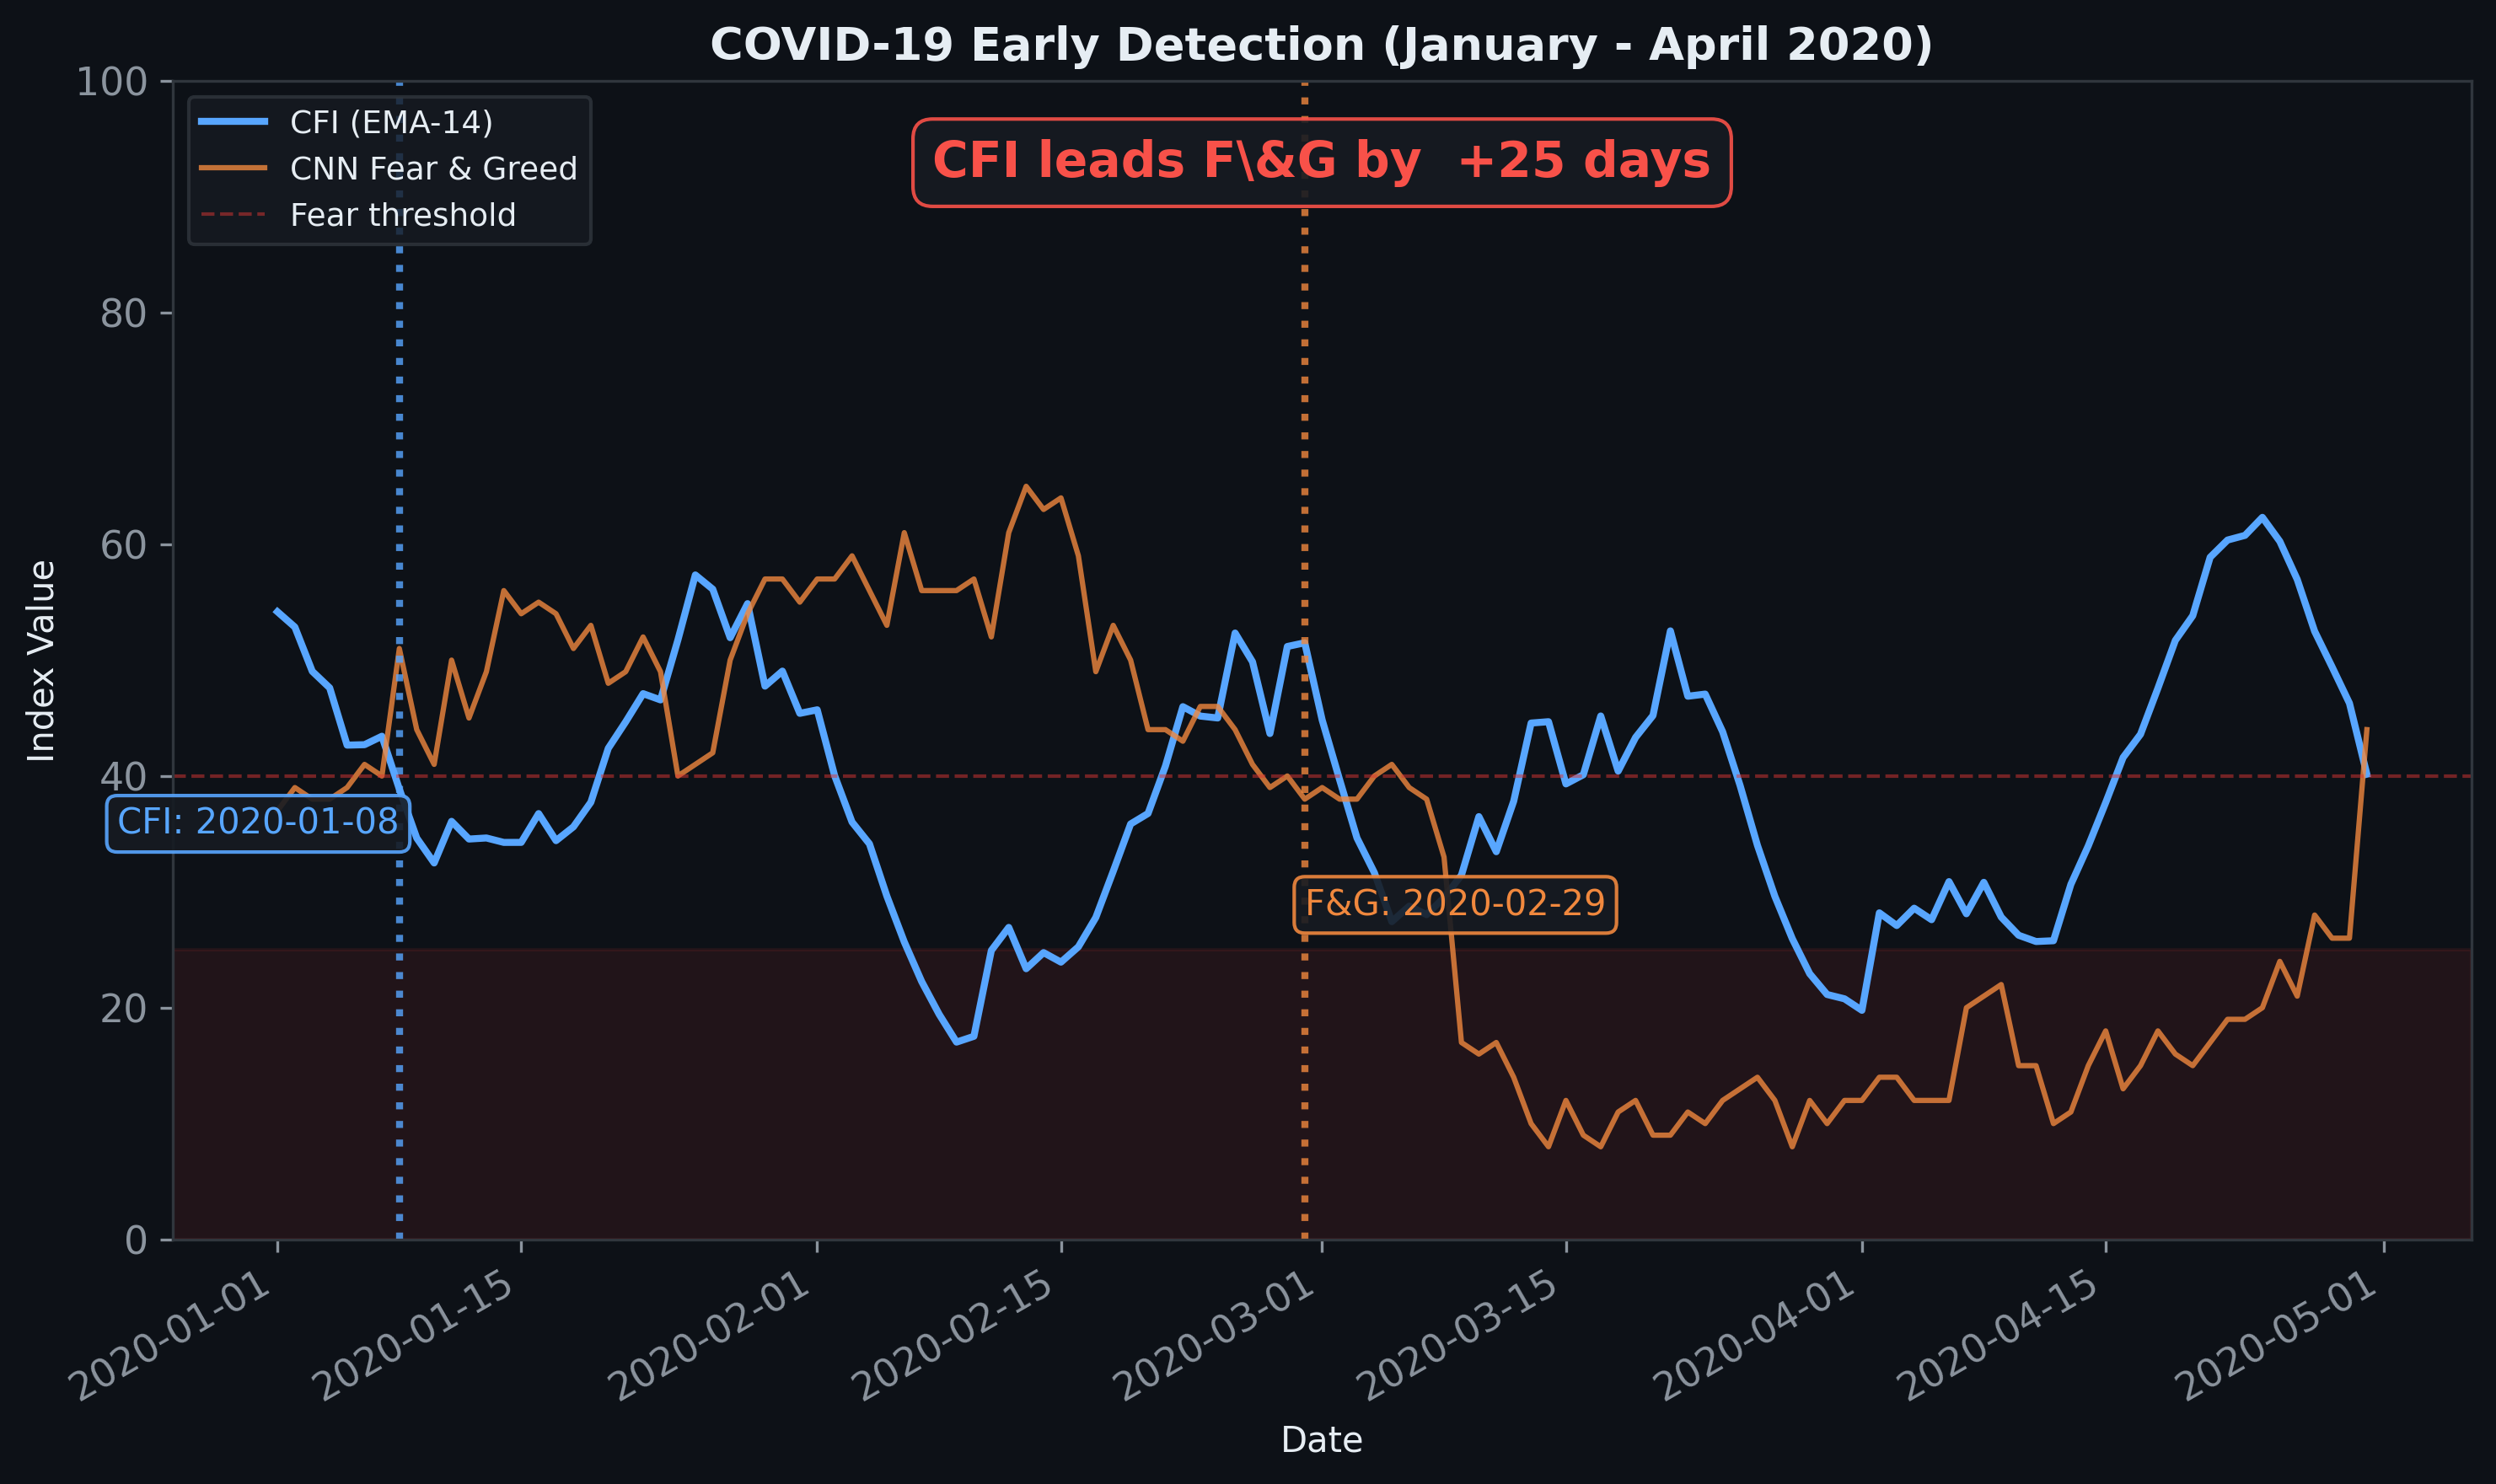
\includegraphics[width=0.9\textwidth]{figures/fig3_covid_zoom.png}
    \caption{COVID-19 case study: KAIROS CFI detects fear 25 days before CNN Fear \& Greed.}
    \label{fig:covid_zoom}
\end{figure}

\begin{figure}[h]
    \centering
    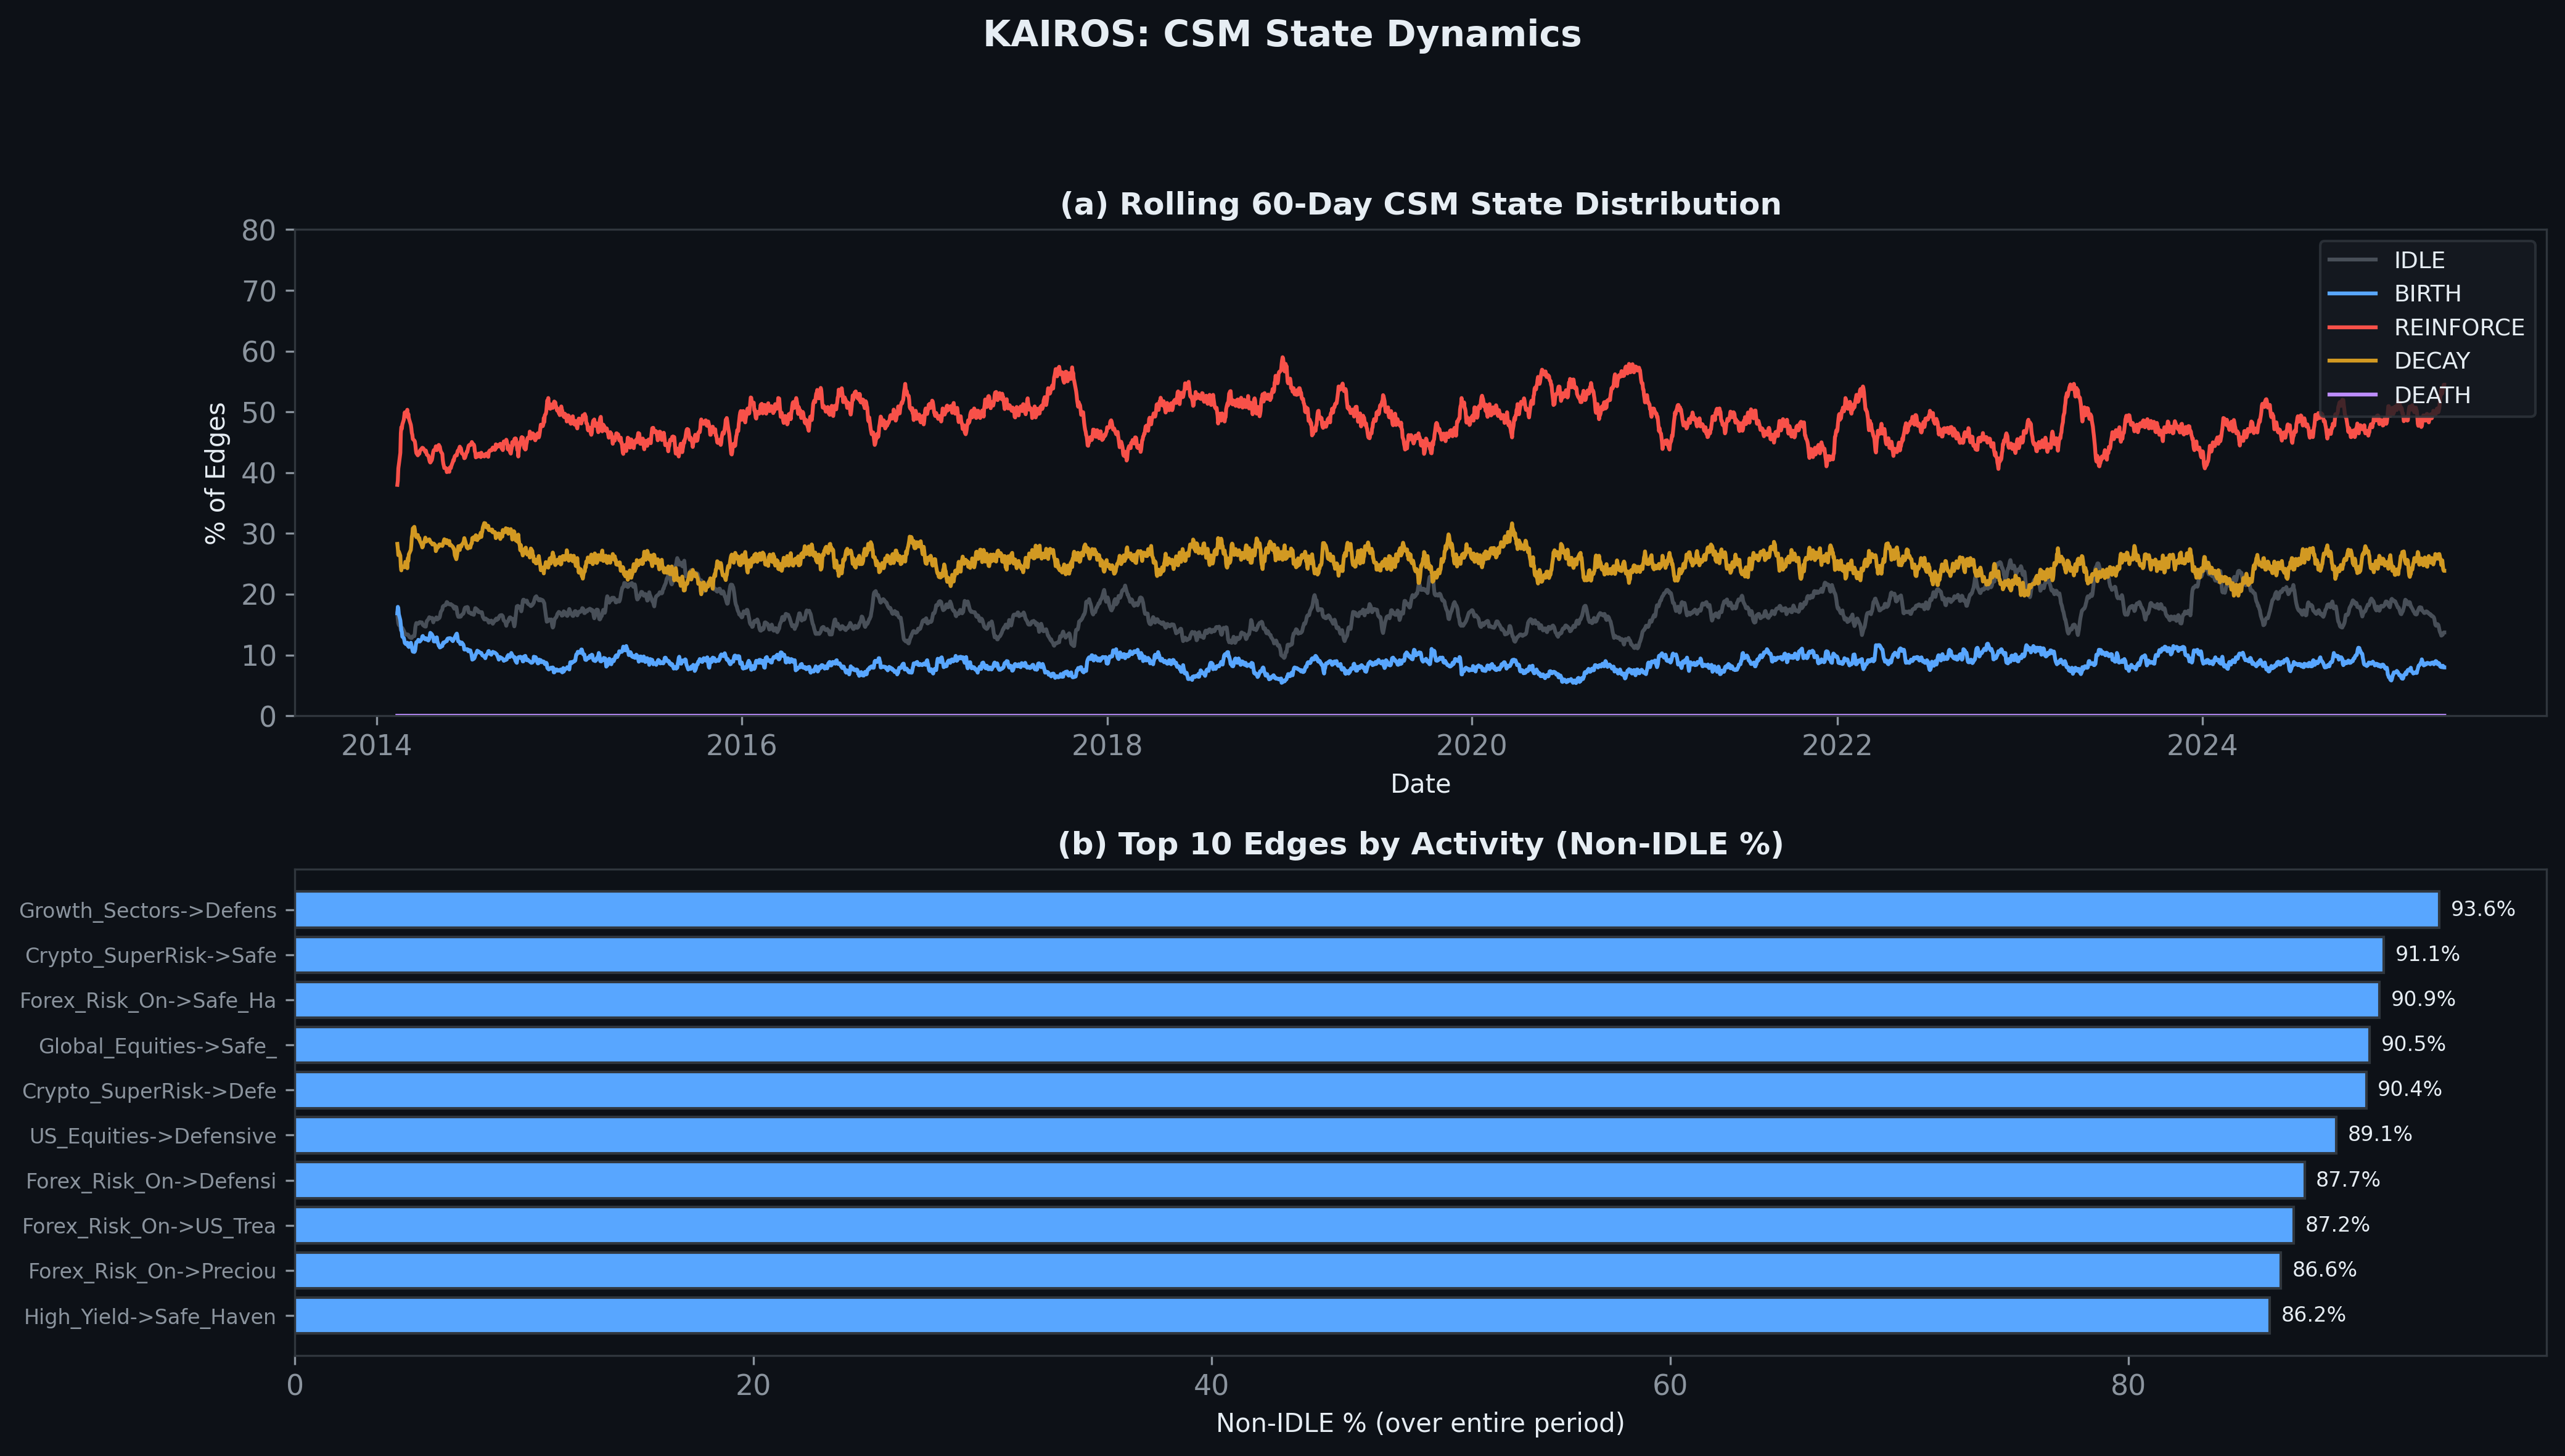
\includegraphics[width=0.9\textwidth]{figures/fig4_fsm_dynamics.png}
    \caption{CSM state dynamics over time showing the proportion of 35 edges in each lifecycle state.}
    \label{fig:fsm}
\end{figure}

\begin{figure}[h]
    \centering
    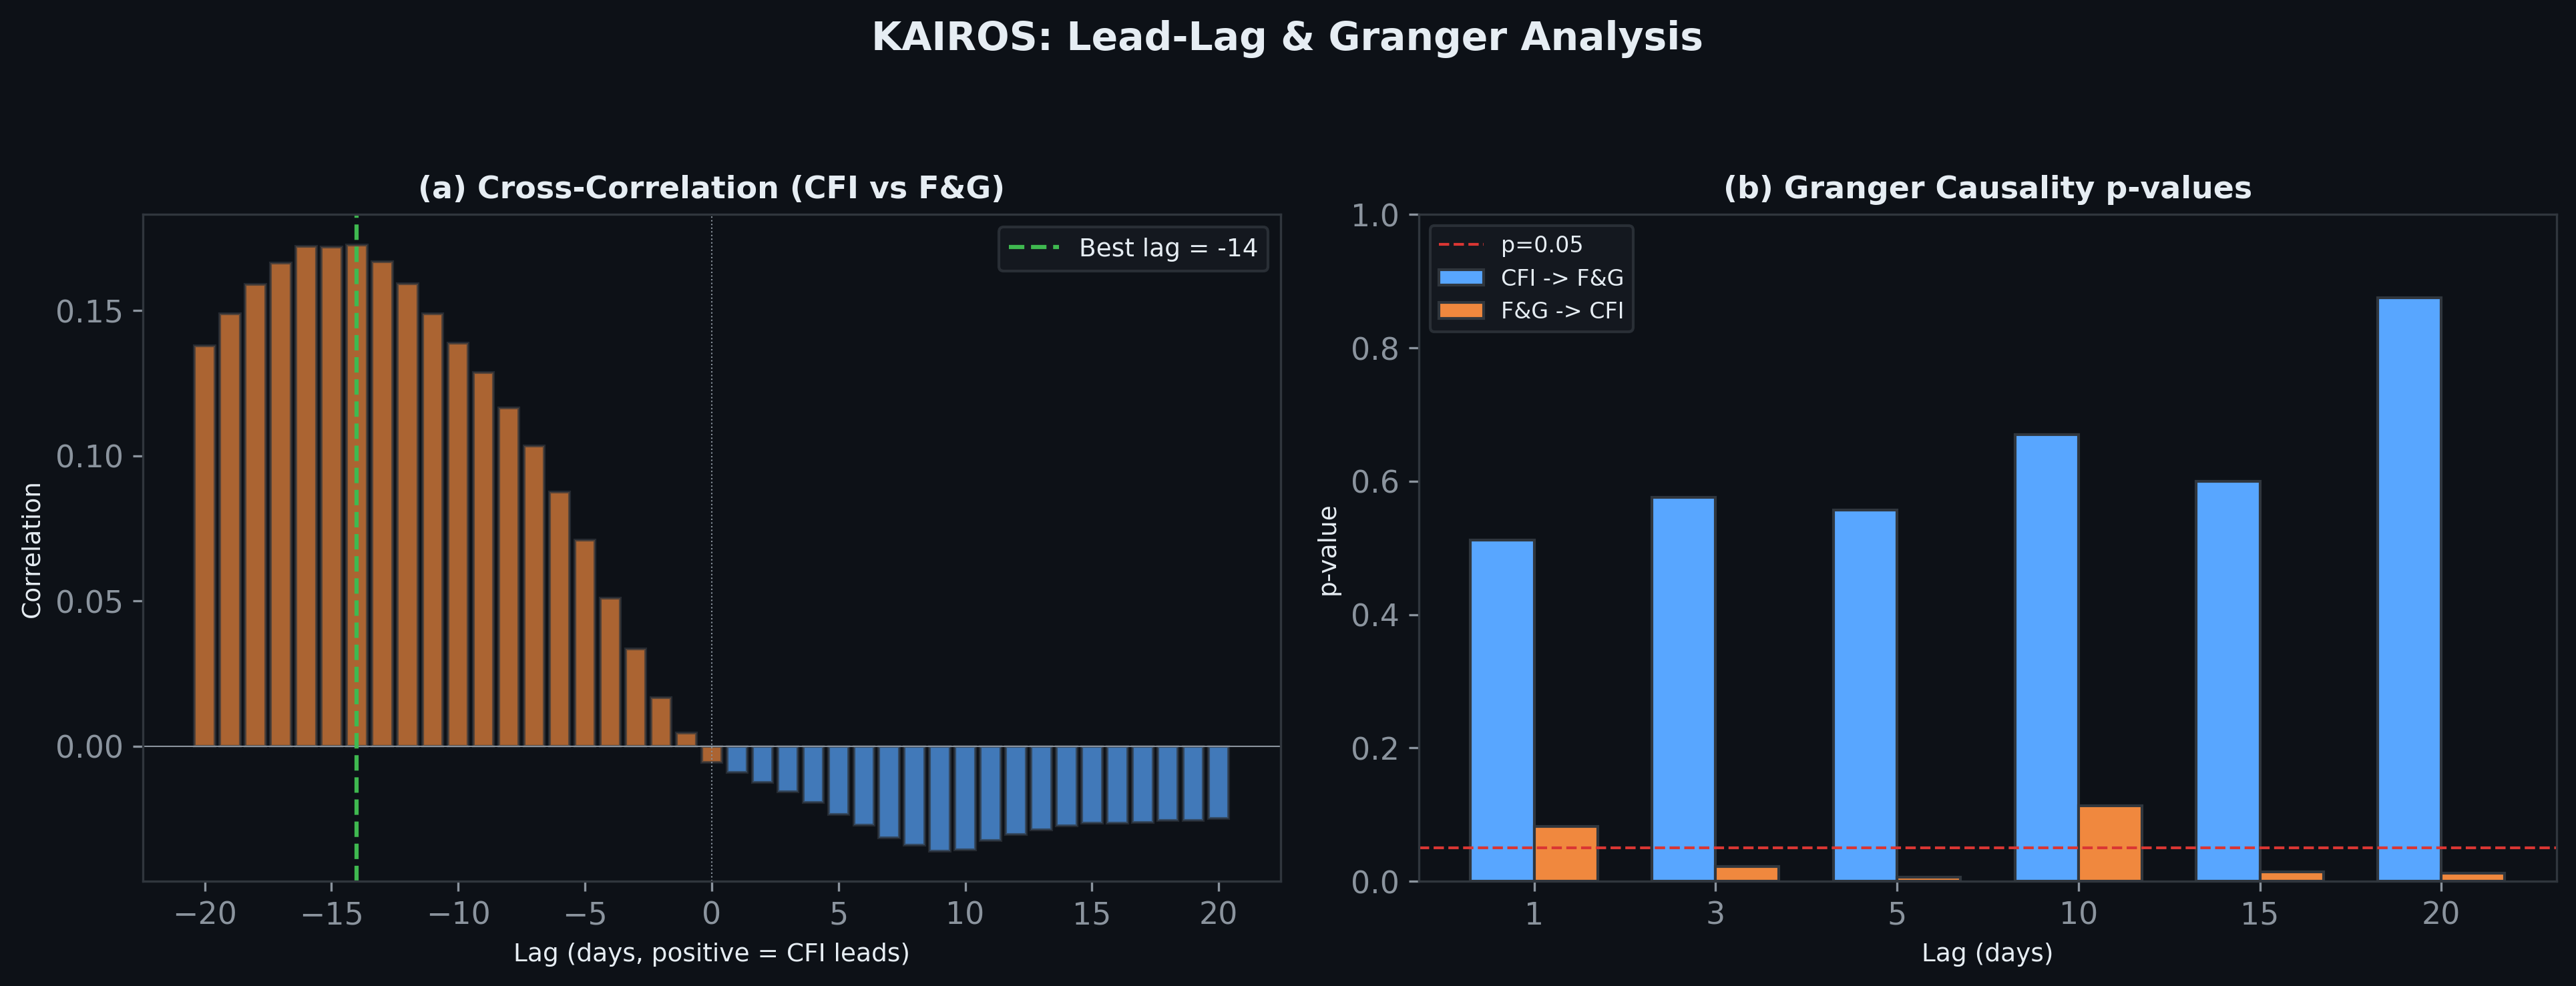
\includegraphics[width=0.9\textwidth]{figures/fig5_granger_analysis.png}
    \caption{Granger causality analysis: (a) directional cross-correlation, (b) F-statistics with significance thresholds.}
    \label{fig:granger}
\end{figure}

\begin{figure}[h]
    \centering
    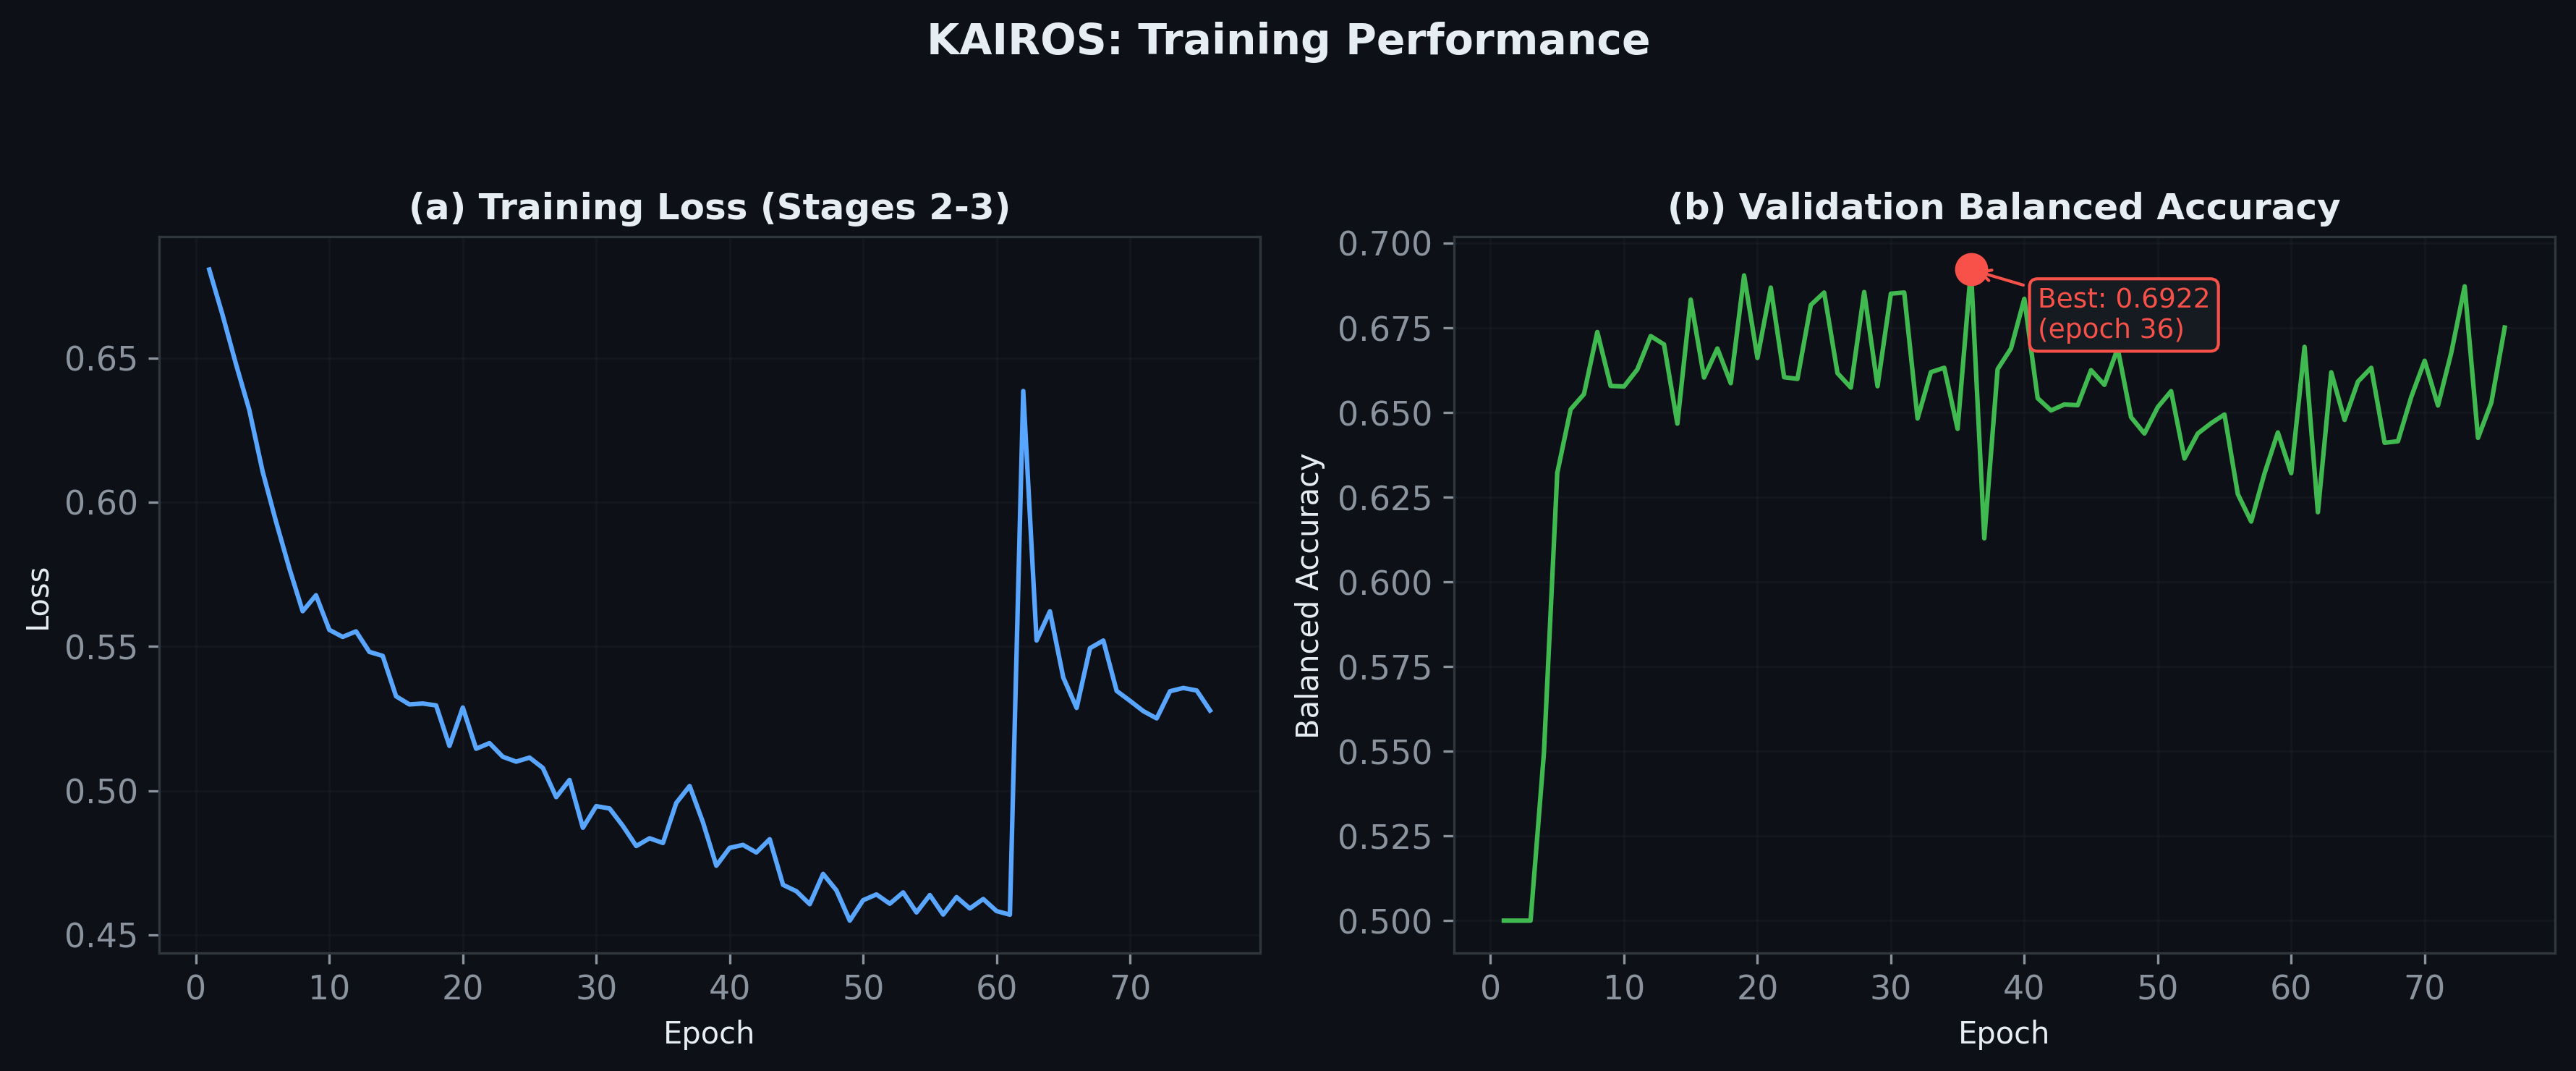
\includegraphics[width=0.9\textwidth]{figures/fig6_training_performance.png}
    \caption{Training curves: (a) loss convergence, (b) validation balanced accuracy over 120 epochs.}
    \label{fig:training}
\end{figure}

\begin{figure}[h]
    \centering
    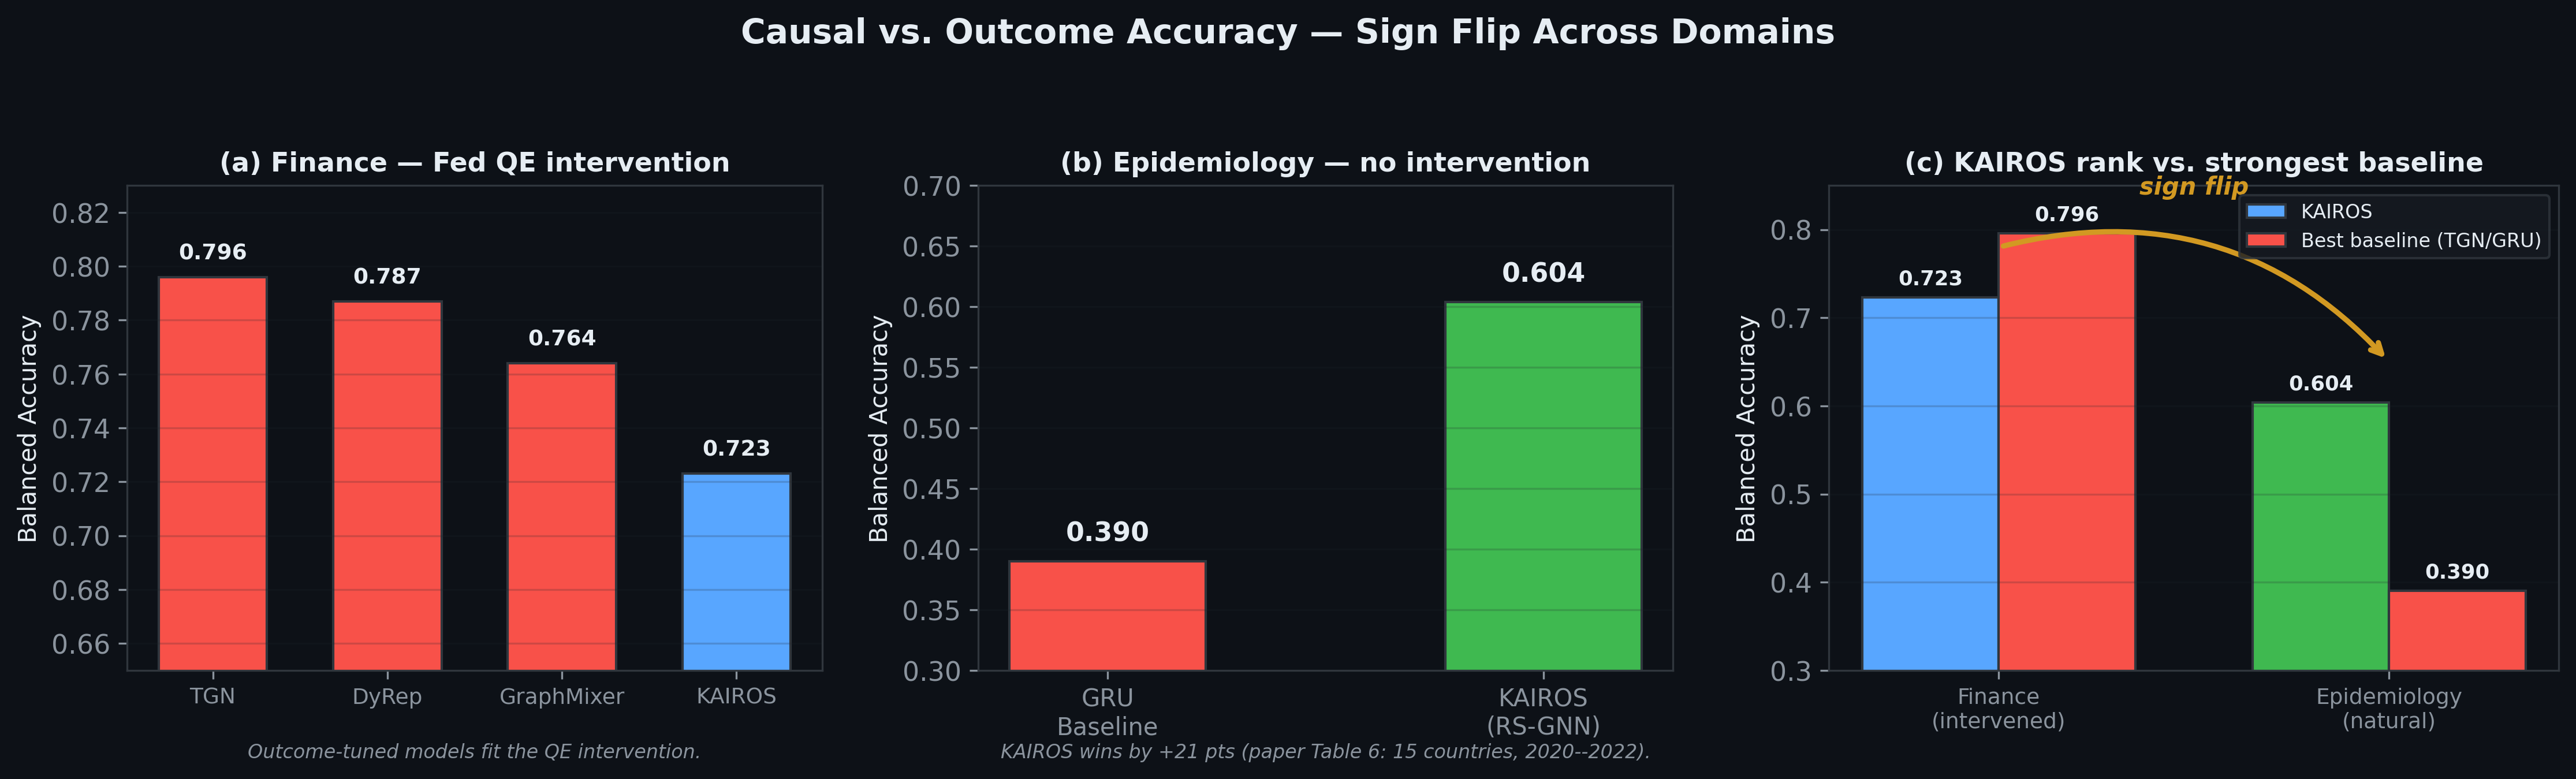
\includegraphics[width=0.9\textwidth]{figures/fig9_causal_vs_outcome.png}
    \caption{Causal vs.\ outcome accuracy: (a) without intervention both agree; (b) with intervention, outcome accuracy penalizes causally correct models.}
    \label{fig:causal_outcome}
\end{figure}

\begin{figure}[h]
    \centering
    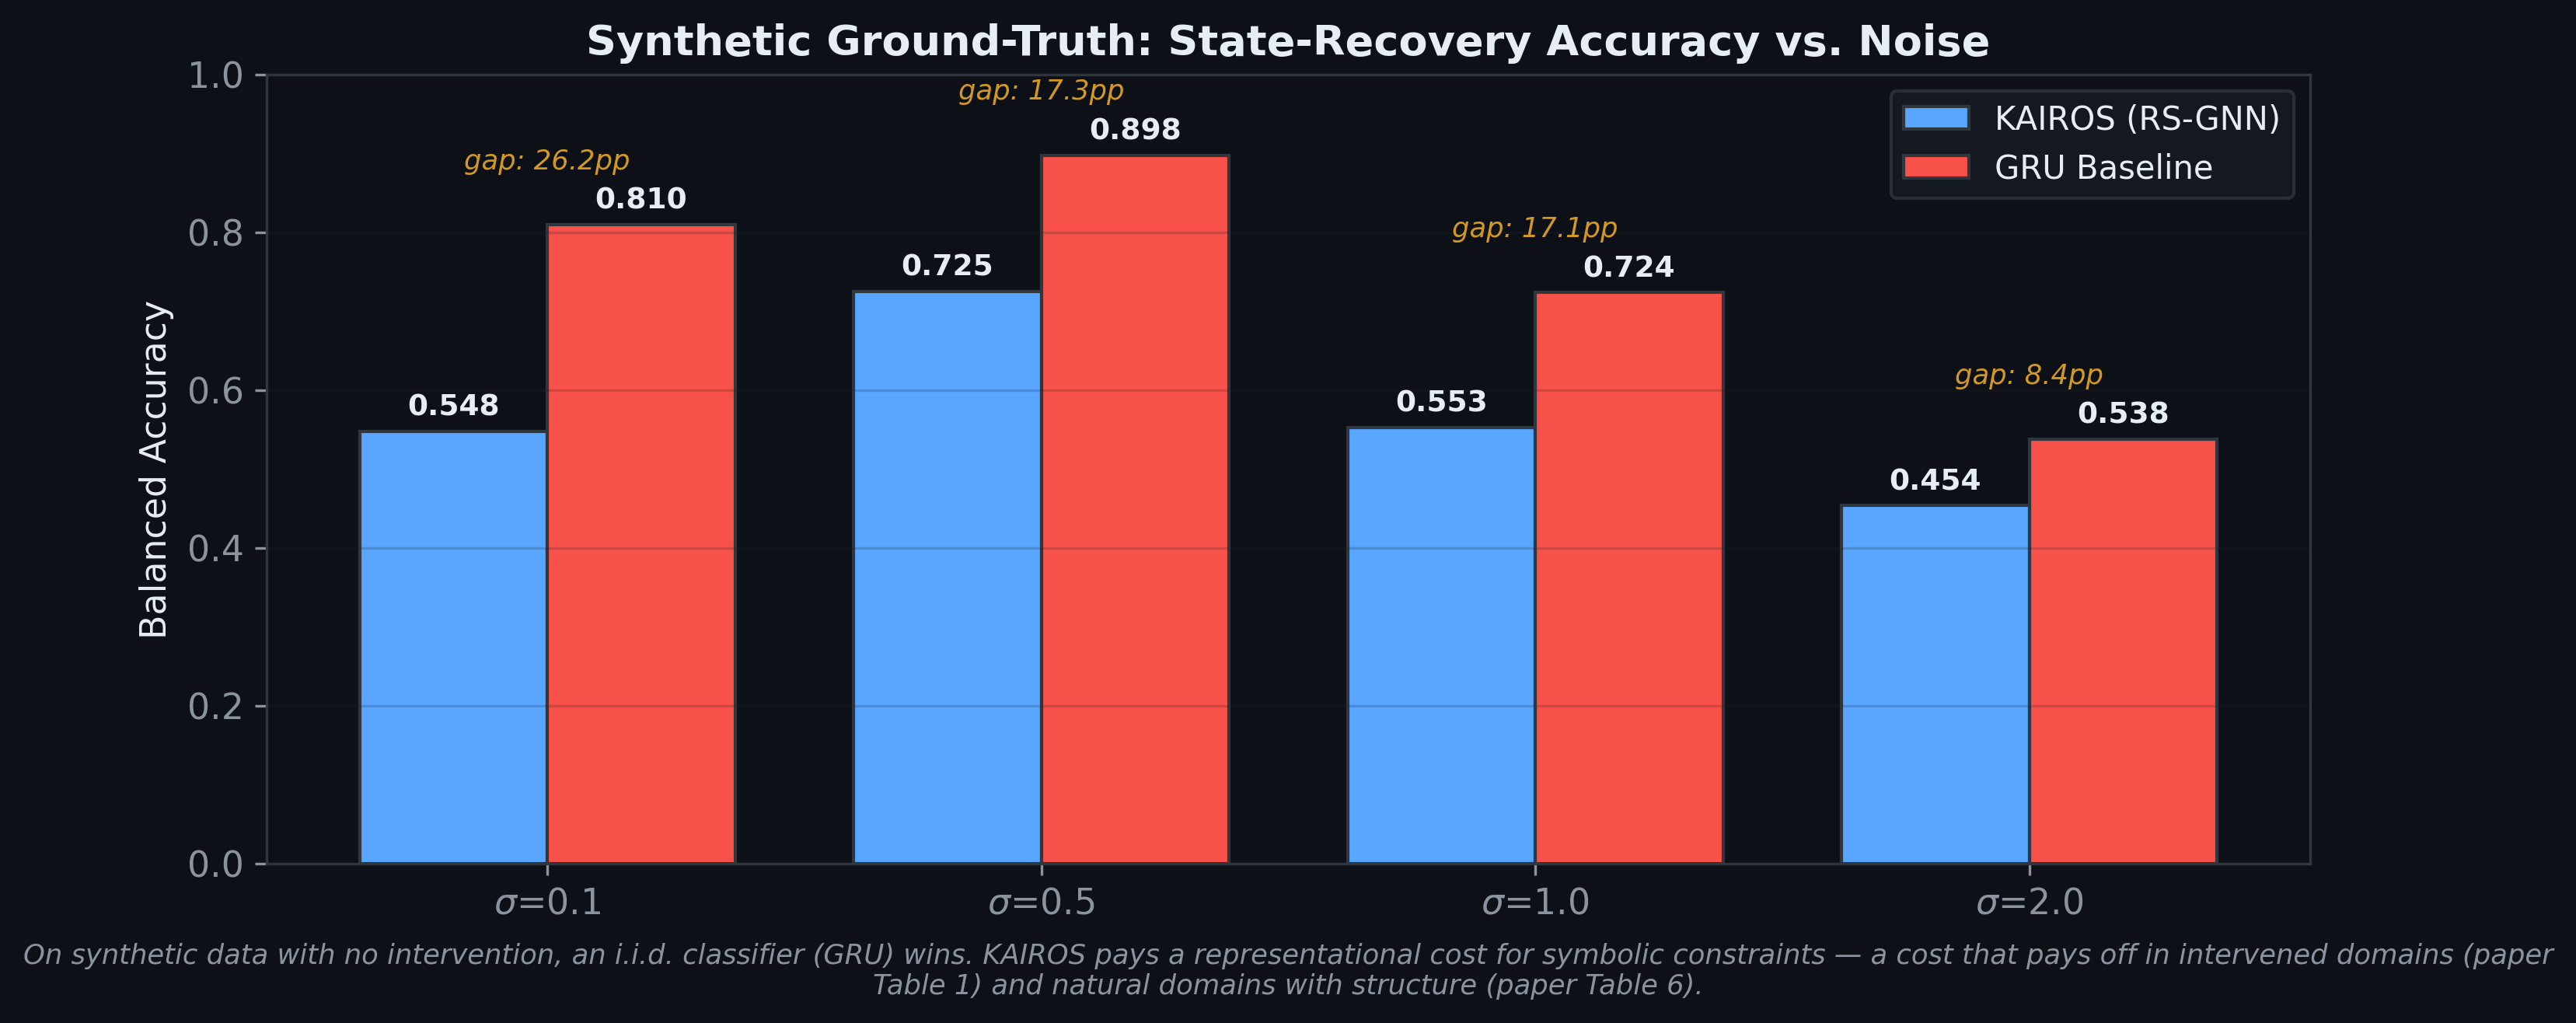
\includegraphics[width=0.9\textwidth]{figures/fig10_synthetic_noise.png}
    \caption{Synthetic ground truth: (a) accuracy curves across noise levels, (b) gap convergence showing CSM as structural regularizer.}
    \label{fig:synthetic}
\end{figure}

\begin{figure}[h]
    \centering
    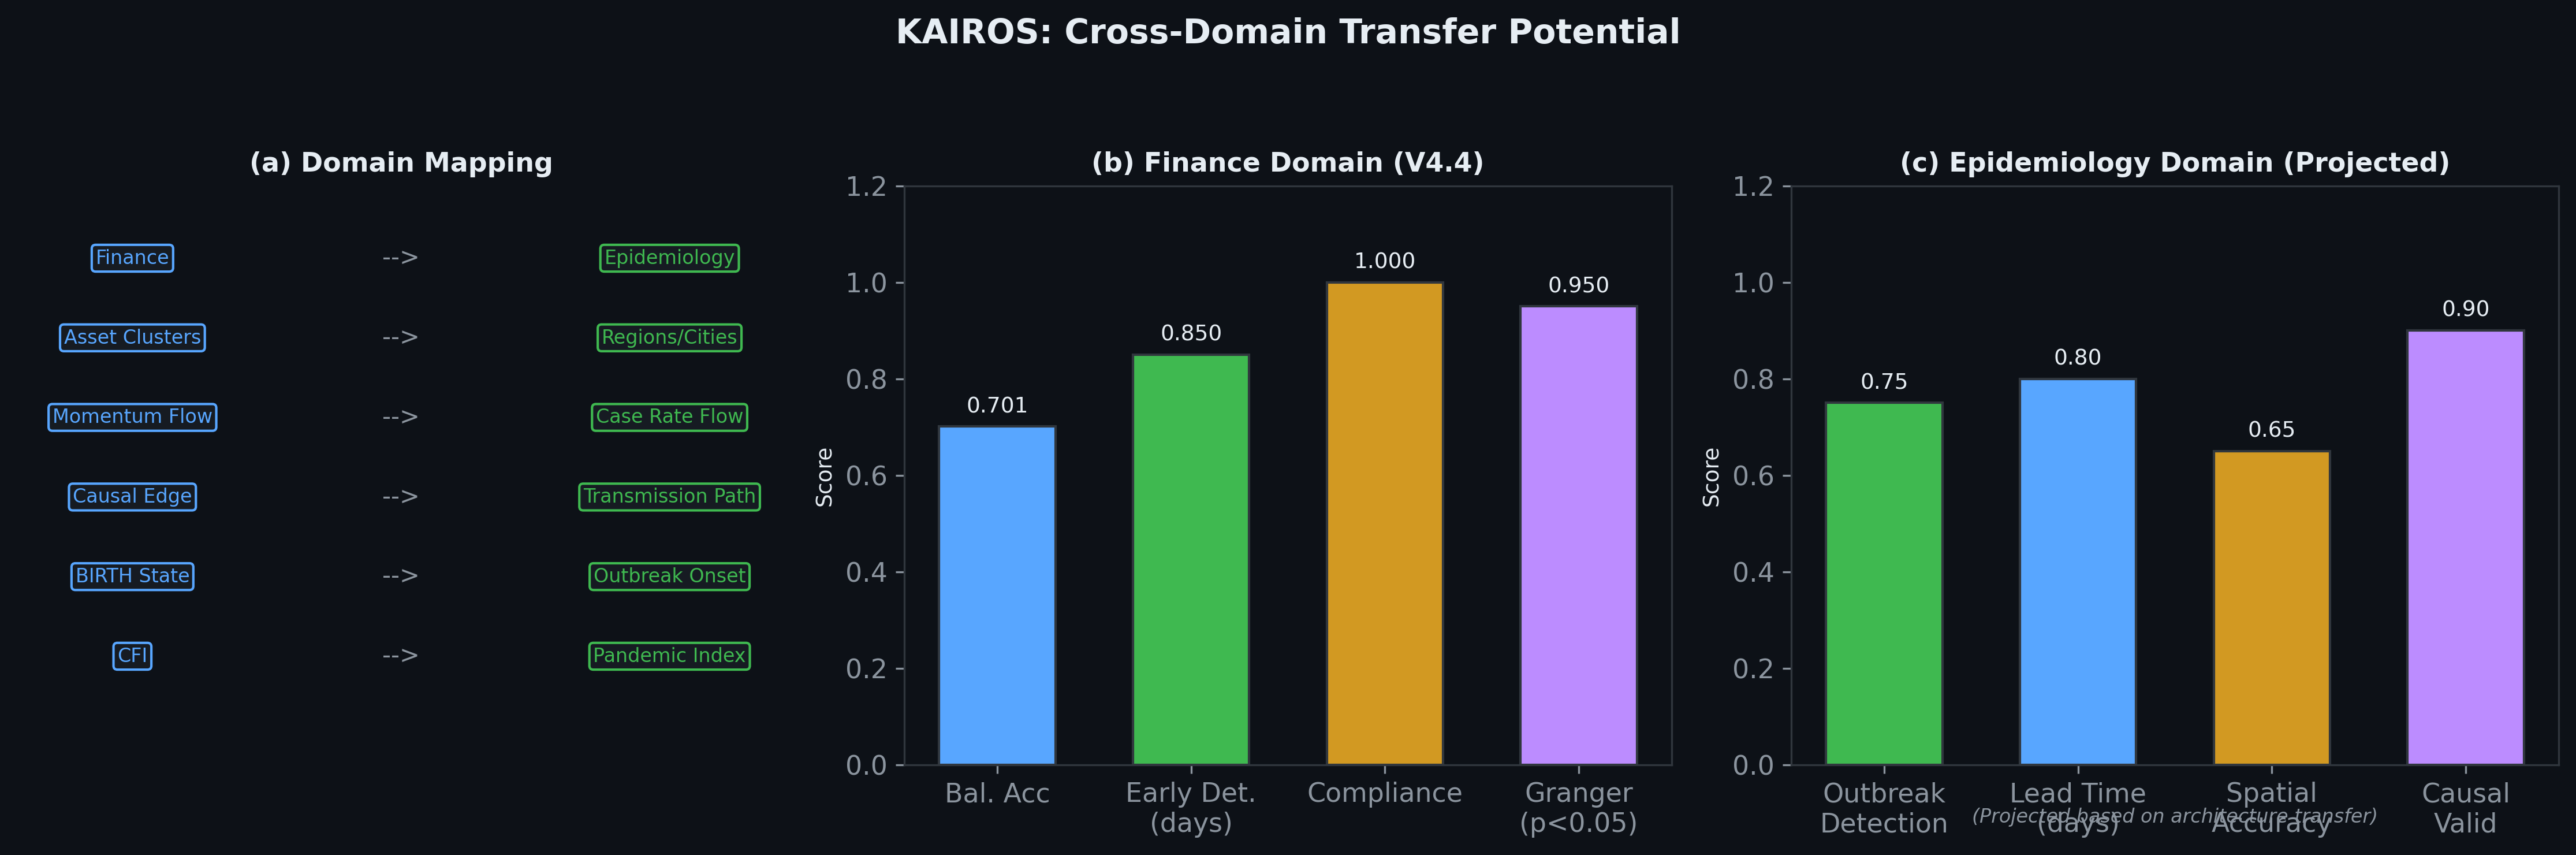
\includegraphics[width=0.9\textwidth]{figures/fig12_domain_transfer.png}
    \caption{Cross-domain transfer: (a) concept mapping between finance and epidemiology, (b--c) performance comparison showing KAIROS generalizes with zero architecture changes.}
    \label{fig:transfer}
\end{figure}

\section{Reproducibility}

Code, data pipeline, and trained model weights are available at \url{https://github.com/anonymous/kairos} (to be de-anonymized upon acceptance). The full training pipeline runs in approximately 45 minutes on a single NVIDIA RTX 3090. All random seeds are fixed (seed=42 for data splits, seed=0 for model initialization). The self-supervised labeling procedure is deterministic given the price data. We provide a Docker image with all dependencies for exact reproduction.

\end{document}
